%Tipus de document
\documentclass[twoside, a4paper, 12pt]{report}

%Paquets que s'utilitzen en aquest document
%Paquets que s'utilitzen en aquest document
\usepackage[a4paper]{geometry} %els marges de la classe book són estrets, amb el paquet geometry es poden modificar
\geometry{margin=2.5cm}
\usepackage{fancyhdr} %el paquet fancyhdr ofereix moltes opcions pel que fa capçalera de les pàgines i número de pàgina, veure: https://tex.stackexchange.com/a/670860/314029

\pagestyle{fancy}
\renewcommand{\chaptermark}[1]{\markboth{#1}{}}

\fancyhf{} % clear the headers
\fancyhead[R]{
   % The chapter number only if it's greater than 0
   \ifnum\value{chapter}>0 \chaptername\ \thechapter. \fi
   % The chapter title
   \leftmark}
\fancyfoot[C]{\thepage}

\fancypagestyle{plain}{
  \renewcommand{\headrulewidth}{0pt}
  \fancyhf{}
  \fancyfoot[C]{\thepage}
}


\usepackage{graphicx} %Required for inserting images
\usepackage[catalan]{babel} %Idioma del document
\usepackage{titlesec} %Paquet per treure el titol capitol x per cada apartat.
\usepackage{float}
    
%Configuracio del titol per cada pagina:
\titleformat{\chapter}[display]
  {\Huge\bfseries}
  {}
  {0pt}
  {\thechapter.\ }

\titleformat{name=\chapter,numberless}[display]
  {\Huge\bfseries}
  {}
  {0pt}
  {}


%...
%Variables que s'utilitzen per personalitzar la portada    
\newcommand{\titol}{Disseny i implementació d'un amplificador d'àudio de tipus D modulat per una FPGA}
\newcommand{\autortesi}{Guillem Ropero Serrano}
\newcommand{\anydediposit}{2025}
\newcommand{\grau}{Grau d'Enginyeria Electronica Industrial i Automàtica}
\newcommand{\director}{Jordi Cosp}

\newcommand{\univeristat}{UPC}

\usepackage{booktabs}
\usepackage{array}
\usepackage{amsmath}
\usepackage{amssymb}
\usepackage{eurosym}
\usepackage{hyperref}
\hypersetup{
    colorlinks=true,
    linkcolor=blue,
    filecolor=black,      
    urlcolor=blue,
    pdftitle={Disseny i implementació d'un amplificador d'àudio de tipus D},
    pdfpagemode=FullScreen,
    }
\usepackage{listings}
\usepackage{rotating}
\usepackage{longtable}
\usepackage{caption}
\usepackage{subcaption}
%\usepackage[square,numbers]{natbib}
%\usepackage[backend=biber,style=apa]{biblatex}
%\bibliographystyle{ieeetr}
%\addbibresource{export}
%\bibliography{export}

\begin{document}


\begin{titlepage}


\newcommand{\HRule}{\rule{\linewidth}{0.5mm}} % Defines a new command for the horizontal lines, change thickness here

% Logo
\centering

\includegraphics[width=8cm]{upc-positiu-p3005.png}\\[1cm] 
 
\center 

\textsc{\LARGE Treball Fi de Grau}\\[1.5cm] 
\textsc{\large \grau}\\[0.5cm] 
\textsc{\Large Memòria i Annexos}\\[0.5cm] 

% Title
\makeatletter
\HRule \\[0.4cm]
{ \huge \bfseries \titol}\\[0.4cm] % Title of your document
\HRule \\[1.5cm]
 
% Author

\begin{minipage}{0.4\textwidth}
\begin{flushleft} \large
\emph{Autor:}\\
\autortesi 


\end{flushleft}
\end{minipage}
~
\begin{minipage}{0.4\textwidth}
\begin{flushright} \large
\emph{Director:} \\
Prof. Jordi Cosp Vilella \\[1.2em] 
\end{flushright}
\end{minipage}\\[2cm]
\makeatother

% Date

{\large Convocatòria: Gener 2025}\\[2cm]

\begin{figure}[H]
\centering
  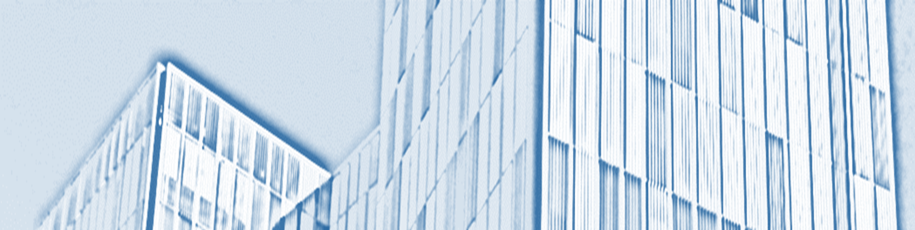
\includegraphics[width=15cm]{logo_eebe_portada.png}
\end{figure}
\end{titlepage}

\vfill % Fill the rest of the page with whitespace

\chapter*{Resum}
\par Aquest treball de final de grau té com a objectiu el disseny i implementació d'un sistema de processament digital i amplificació d'àudio utilitzant una placa de desenvolupament d'una FPGA. El projecte es centra a desenvolupar un amplificador d'àudio de tipus D, conegut per la seva alta eficiència energètica, integrat amb un sistema de processament digital d'àudio (DSP).

\par Mitjançant l'ús d'una FPGA, s'exploren les possibilitats d'un processament digital altament personalitzable i de baix consum. L'estudi inclou el disseny de l'etapa de filtratge i modelat de soroll, la programació de la FPGA, i la validació del sistema complet, demostrant la viabilitat tècnica i pràctica de la proposta. Aquest treball posa en evidència el potencial de les FPGAs com a plataformes versàtils per al desenvolupament de sistemes d'àudio moderns.

\par En el present treball s'ha aconseguit implementar a la FPGA un bloc receptor I2S, una etapa de filtratge i sobremostreig de OSR = 32 i un modulador $\Sigma \Delta$ de segon ordre, donant com a resultat que el senyal d'àudio de l'entrada es pugui reproduir mitjançant l'ús d'uns auriculars. 
\addcontentsline{toc}{chapter}{\protect\numberline{}Resum}


\chapter*{Resumen}
\par Este trabajo de fin de grado tiene como objetivo el diseño e implementación de un sistema de procesamiento digital y amplificación de audio utilizando una placa de desarrollo con una FPGA. El proyecto se centra en desarrollar un amplificador de audio de tipo D, conocido por su alta eficiencia energética, integrado con un sistema de procesamiento digital de audio (DSP).

\par Mediante el uso de una FPGA, se exploran las posibilidades de un procesamiento digital altamente personalizable y de bajo consumo. El estudio incluye el diseño de la etapa de filtrado y modelado de ruido, la programación de la FPGA y la validación del sistema completo, demostrando la viabilidad técnica y práctica de la propuesta. Este trabajo pone de manifiesto el potencial de las FPGAs como plataformas versátiles para el desarrollo de sistemas de audio modernos.

\par En el presente trabajo se ha logrado implementar en la FPGA un bloque receptor I2S, una etapa de filtrado y sobremuestreo con OSR = 32, y un modulador $\Sigma \Delta$ de segundo orden, resultando en que la señal de audio de salida se reproduzca a través de unos auriculares.

\addcontentsline{toc}{chapter}{\protect\numberline{}Resumen}


\chapter*{Abstract}
\par This final degree project aims to design and implement an audio processing and amplification system using an FPGA. The project focuses on developing a Class D audio amplifier, known for its high energy efficiency, integrated with a digital signal processing (DSP) audio system.  

\par By leveraging the capabilities of an FPGA, the study explores the possibilities of highly customizable and low-power digital processing. The research includes the design of the filtering and noise-shaping stages, the programming of the FPGA, and the validation of the complete system, demonstrating the technical and practical feasibility of the proposal. This work highlights the potential of FPGAs as versatile platforms for the development of modern audio systems.

\par In the present work, an I2S receiver block, a filtering and oversampling stage with OSR = 32, and a second-order $\Sigma \Delta$ modulator have been successfully implemented on the FPGA resulting in the output audio signal being played through headphones.

\addcontentsline{toc}{chapter}{\protect\numberline{}Abstract}
\chapter*{Agraïments}
\par A la meva familia pel suport incondicional durant la realització d'aquest treball. Al tutor d'aquest treball, Jordi Cosp, pel seu suport tècnic i a l'associcació d'e-Tech Racing i els seus membres, amb qui he passat els millors moments d'aquesta carrera. 

\addcontentsline{toc}{chapter}{\protect\numberline{}Agraïments}
\tableofcontents
\listoffigures
\listoftables

\chapter*{Glossari}
\addcontentsline{toc}{chapter}{\protect\numberline{}Glossari}
\begin{longtable}[H]{ll}
\textbf{I2S} & Inter-Integrated Circuit Sound
\\
\textbf{DSP} & Digital Signal Processing
\\
\textbf{FPGA} & Field-Programmable Gate Arrays
\\
\textbf{FET} & Field Effect Transistors
\\
\textbf{PWM} & Pulse Width Modulation
\\
\textbf{PDM} & Pulse Density Modulation
\\
\textbf{IC} & Integrated Circuit
\\
\textbf{VLSI} & Very Large Scale Integration
\\
\textbf{CLB} & Configurable Logic Blocks
\\
\textbf{SoC} & System on Chip
\\
\textbf{LUT} & Look Up Table
\\
\textbf{MAC} & Multiply and Accumulate
\\
\textbf{DSP} & Digital Signal Processing
\\
\textbf{CD} & Compact Disk
\\
\textbf{LSB} & Least Significant Bit
\\
\textbf{MSB} & Most Significant Bit
\\
\textbf{SCLK} & Serial Clock
\\
\textbf{BCLK} & Bit Clock
\\
\textbf{DSP} & Digital Signal Processing
\\
\textbf{WS} & Word Select
\\
\textbf{FIR} & Finite Impulse Response
\\
\textbf{CIC} & Cascaded Integrator-Comb
\\
\textbf{IIR} & Infinite Impulse Response
\\
\textbf{STF} & Signal Transfer Function
\\
\textbf{NTF} & Noise Transfer Function
\\
\textbf{CIFB} & Cascaded Integrator Feedback
\\
\textbf{CRFB} & Cascaded Resonator Feedback
\\
\textbf{CIFF} & Cascaded Integrator Feedforward
\\
\textbf{CRFF} & Cascaded Resonator Feedforward
\\
\textbf{SNR} & Signal to Noise Ratio
\\
\textbf{DR} & Dynamic Range
\\
\textbf{THD} & Total Harmonic Distorsion
\\
\textbf{FS} & Full Scale
\\
\textbf{SPI} & Serial Port Interface
\\
\textbf{RAM} & Random Access Memory
\\
\textbf{SD} & Secure Digital
\\
\textbf{RTOS} & Real Time Operating System
\\
\textbf{SIPO} & Serial-Input Parallel-Output
\\
\textbf{PIPO} & Parallel-Input Parallel-Output
\\
\textbf{VHDL} & Very High Speed Integrated Circuits Hardware Description Language
\\
\textbf{OSR} & Over-Sampling Ratio
\\
\textbf{EEBE} & Escola d'Enginyeria de Barcelona Est
\\
\textbf{SMI} & Salari Mínim Interprofessional
\\
\textbf{ECTS} & European Credit Transfer System
\end{longtable}
\chapter{Introducció}
\section{Presentació del treball}
\par La concepció d'aquest treball sorgeix de l'interès de l'autor per l'electrònica digital i analògica, i de demostrar les avantatges d'implementar sistemes que es beneficiïn dels dos vessants. Es planteja doncs el disseny i implementació d'un amplificador d'àudio de tipus D, que com es comentarà més endavant, es poden obtenir altes prestacions a la sortida amb tècniques de processament digital.  
\par La tecnologia d'àudio digital està substituint progressivament la majoria dels dispositius i tasques que tradicionalment es duien a terme amb components analògics. Aquesta tecnologia es pot considerar com una evolució de les pràctiques i tècniques desenvolupades durant dècades en l'àmbit de l'electroacústica i l'enginyeria d'àudio. Tot i això, la conversió digital dels senyals comporta el risc de pèrdues significatives en la qualitat del so si no es prenen les mesures adequades. Mitjançant tècniques com el filtratge i el modelatge del soroll, és possible obtenir una qualitat d'àudio elevada de manera eficient. A més, el processament digital de senyals ofereix avantatges significatius respecte al tractament analògic, especialment pel que fa a la reducció del consum energètic, fet que el converteix en una alternativa més sostenible i eficient en molts casos. 
\par Per a la implementació de sistemes de processament digital de senyals (DSP), l’ús de FPGAs (Field-Programmable Gate Arrays) es presenta com una de les millors opcions. Les FPGAs permeten una flexibilitat i paral·lelisme que són difícils d’assolir amb altres arquitectures, com ara microprocessadors o DSPs dedicats. Aquesta característica les fa especialment adequades per a aplicacions on es requereix un alt rendiment en temps real, com ara en sistemes d'àudio digital. A més, les FPGAs permeten personalitzar l'arquitectura per optimitzar l'ús de recursos i el consum energètic, adaptant-se de manera òptima als requisits específics del projecte. Per aquestes raons, les FPGAs són una eina clau en el desenvolupament d’amplificadors d’àudio de tipus D, ja que poden gestionar amb precisió la modulació i el filtratge digital, garantint unes prestacions excel·lents tant en eficiència com en qualitat sonora.

\par Mitjançant l'ús de tècniques avançades de processament digital de senyals, es pretén aconseguir un sistema altament eficient, amb un consum energètic reduït i unes prestacions acústiques de qualitat elevada. A més, es posa èmfasi en la versatilitat d'aquests sistemes i en la seva capacitat per superar els límits dels enfocaments exclusivament analògics o digitals. Finalment, en aquest treball es dissenyarà una etapa de recepció d'àudio en protocol I2S, una etapa de filtratge i un modulador $\Sigma \Delta$ amb l'objectiu de fer sonar uns auriculars amb un so nítid.

\section{Objectius}
\par Per a la realització d'aquest treball es defineixen els següents objectius amb la intenció d'implementar una etapa completa d'àudio funcional i adquirir coneixements en la matèria de processament digital de senyals. A continuació s'enumeren els objectius que s'ha fixat en la realització d'aquest treball.
\begin{itemize}
    \item Objectiu 1: Implementar un bloc IP receptor per fer lectures en protocol I2S.
    \item Objectiu 2: Dissenyar i implementar etapes de filtrat per l'àudio a l'entrada i sobremostrejar el senyal.
    \item Objectiu 3: Dissenyar i implementar un modulador $\Sigma \Delta$ que modeli el soroll provocat per la quantificació.
    \item Objectiu 4: Dissenyar una etapa de delmat del senyal d'àudio provinent del bloc $\Sigma \Delta$.
\end{itemize}
\par En la valoració final del que s'acabi implementant, es farà un incís per analitzar si s'han complert tots els objectius. 

\section{Amplificadors d'àudio de Classe D}
\par Els amplificadors de classe D són una topologia d'amplificadors electrònics dissenyats per oferir una gran eficiència energètica on els transistors de l'etapa de sortida treballen en règim de commutació i no en règim lineal. En el nivell més elemental de la teoria, l'eficiència d'un amplificador de classe D sempre és del 100\%, a tots els nivells de sortida. A la pràctica, les idealitzacions matemàtiques no es mantenen, i l'eficiència a la vida real dels amplificadors de classe D cau en fins al 80 i 90 \% en la major part del rang de potència a la sortida. Aquestes pèrdues s'originen per diferents mecanismes: 

\begin{itemize}
	
	\item Pèrdues en els transistors a la sortida: Els transistors de l'etapa de sortida tenen una resistència de conducció no nul·la quan estan en règim de saturació, fet que origina pèrdues per $I^{2}R$. A més a més, s'afegeixen les pèrdues per commutació que es veuen agreujades pels components paràsits en els FET.
	
	\item Polsos de retrocés: Degut a la naturalesa inductiva de la càrrega, durant les transicions de nivell es genera una variació del flux magnètic a la bobina, la qual dona lloc a fenòmens transitoris. Aquests fenòmens poden activar els díodes paràsits inherents als FET, provocant la seva conducció no desitjada. Aquests díodes, amb un temps de recuperació inversa relativament llarg, permeten la circulació d’un corrent superior al necessari, cosa que pot afectar l’eficiència del sistema i incrementar les pèrdues energètiques.
	
	\item Shoot-through: Aquest terme fa referència a la situació en què els dos transistors d'un semipont estan conduint al mateix temps. Això provoca un curtcircuit gairebé directe entre els raïls d’alimentació. Per evitar-ho, el circuit de control dels transistors incorporen un temps mort entre transicions de conducció.
	
\end{itemize}

\par El senyal d'àudio d'entrada es modula en un senyal de control digital que impulsa els dispositius de potència a l'etapa de sortida. Aquest senyal es pot modular, normalment, mitjançant modulació d'amplada de pols (PWM) o modulació de densitat de pols (PDM).

\par L'etapa de sortida es pot implementar mitjançant una topologia de Half-Bridge o Full-Bridge, il·lustrada a les figures \ref{fighalfbridge} i \ref{figFullbridge}. Els amplificadors de classe D sovint funcionen en una configuració de pont per augmentar la potència de sortida sense augmentar les tensions d'alimentació. L'última etapa, el filtre de pas baix, s'utilitza per eliminar la freqüència portadora PWM/PDM d'alta freqüència, recuperant així el senyal d'àudio original\cite{SDMClassD}.
\begin{figure}[H]
    \centering
    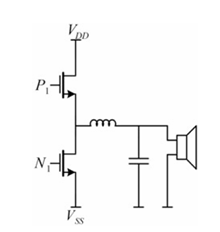
\includegraphics[width=0.25\linewidth]{Images/halfbridge.png}
    \caption{Amplificador de classe D en configuració de semi-pont.}
    \label{fighalfbridge}
\end{figure}
\begin{figure}[H]
    \centering
    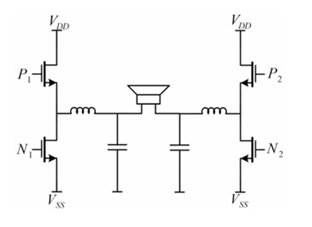
\includegraphics[width=0.3\linewidth]{Images/full-bridge.png}
    \caption{Amplificador de classe D en configuració de pont complet.}
    \label{figFullbridge}
\end{figure}

\subsubsection{Amplificadors de Classe D comercials}
\par En aquest apartat es presenten amplificadors de classe D i DSPs units disponibles en el mercat, i es desglossen les prestacions més rellevants.
\begin{itemize}
    \item AX5688: Amplificador digital de classe D amb entrada d'àudio en protocol I2S, etapa de filtrat i etapa de potència, integrat en el mateix IC. Té 2 sortides PWM que es poden configurar per atacar 2 altaveus en configuració semi-pont o un altaveu en pont complet. Rang Dinàmic = 115 dB; THD+N = -100 dB. \cite{MPSAmpD}
    \item TAS2320: Amplificador digital de classe D amb entrad mono en protocol I2S i etapa de potència de 15 W. L'etapa de potència només pot atacar un altaveu en configuració de semi-pont. Rang Dinàmic = 109dB; THD+N = -89 dB. \cite{TIAmpD}
    \item MAX98365: Amplificador digital de classe D mb entrada d'àudio en protocol I2S i etapa de potència fins 17.6 W. L'etapa de potència només pot atacar un altaveu en configuració de semi-pont. Rang Dinàmic = 111,5 dB; THD+N = -85 dB.\cite{AnalogAmpD}
\end{itemize}

\section{FPGA}
\par Les FPGA són circuits integrats (IC) d'integració a gran escala (VLSI) que poden contenir centenars de milers de blocs lògics configurables (CLB), desenes de milers de blocs funcionals de maquinari predefinits, centenars d'interfícies externes predefinides, milers de blocs de memòria, milers de pads d'entrada/sortida (I/O) i fins i tot un SoC totalment predefinit en determinades famílies FPGA. Aquests elements funcionals es distribueixen de manera òptima per l'àrea de silici de la FPGA i es poden interconnectar mitjançant recursos d'encaminament programables. Això els permet comportar-se d'una manera funcional desitjada per un dissenyador lògic de manera que puguin complir determinades especificacions de disseny i requisits del producte. \cite{Maaref2023} 
\begin{figure}[H]
    \centering
    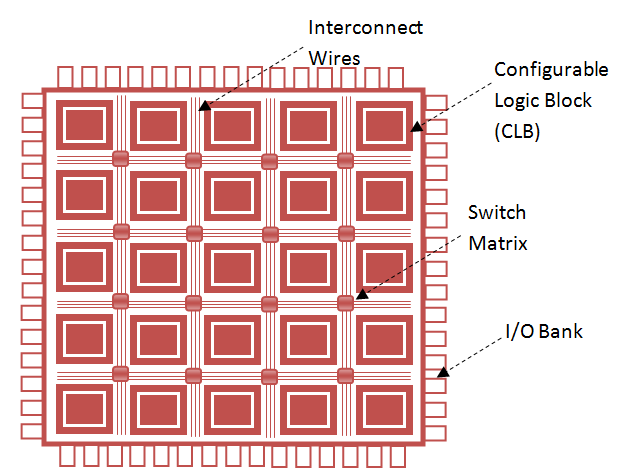
\includegraphics[width=0.5\linewidth]{Images/FPGAdiagram.png}
    \caption{Diagrama de blocs dels elements en una FPGA en el silici del IC.}
    \label{figFPGA}
\end{figure}
\par A diferència dels processadors, els FPGA són capaços de fer operacions paral·leles, de manera que diferents operacions de processament no competeixen pels mateixos recursos. Cada tasca independent s'assigna a una secció dedicada del xip i pot funcionar de manera autònoma sense influència d'altres blocs lògics. En conseqüència, el rendiment d'una part de l'aplicació no es veu afectat a mesura que s'afegeixen més operacions.
\par Les FPGA contenen components especialitzats per a funcions específiques i una lògica configurable de propòsit més general. A continuació es mencionen alguns d'aquests blocs que caracteritzen les FPGAs \cite{FPGADig}:
\begin{itemize}
    \item Configurable Logic Block (CLB): Els blocs lògics configurables (CLB) són la unitat lògica bàsica d'un FPGA. Un CLB dóna a l'FPGA la seva capacitat d'acceptar diferents configuracions de maquinari. Els CLB es poden programar per realitzar gairebé qualsevol funció lògica. El CLB individual conté una sèrie de components lògics discrets, com ara taules de consulta (LUT) i flip-flops.
    \item Flip Flops: Un flip-flop és un circuit que té dos estats estables i es pot utilitzar per emmagatzemar informació. Els flip-flops són registres de desplaçament binaris que sincronitzen la lògica i guarden estats lògics entre cicles de rellotge dins d'un circuit FPGA. Un flip-flop emmagatzema un sol bit de dades.
    \item Look Up Tables (LUT): Determina quina és la sortida per a qualsevol entrada donada. En el context de la lògica combinatòria, és la taula de veritat i defineix com es comporta la lògica combinatòria. Una taula de veritat és una llista predefinida de sortides per a cada combinació d'entrades. El LUT conté una taula de veritat personalitzada que es carrega quan el xip s'engega.
    \item Blocs DSP o MAC: Realitza funcions de processament de senyal digital, com ara filtrar o multiplicar, de manera més eficient que utilitzar molts CLB. Aquest circuit multiplicador estalvia l'ús de LUT i flip-flop en aplicacions de processament de senyal i matemàtiques.
\end{itemize}

\subsubsection{Placa de desenvolupament Nexys4}
\par Pel desenvolupament del projecte i la implementació final, s'ha emprat la placa de desenvolupament Nexys4. La placa inclou la FPGA Artix-7 de Xilinx i múltiples prestacions per diverses aplicacions. A la taula \ref{taulaArtix7} es poden veure plasmades les característiques de la FPGA Artix-7. Per l'aplicació d'aquest treball, destaca l'etapa de filtrat actiu analògica, implementada amb un filtre passabaixos de 4rt ordre en topologia Sallen-Key a la sortida d'àudio en format stereo.
\begin{table}[H]
    \centering
    \begin{tabular}{ | c | }
    \hline
    \textbf{Prestacions FPGA Artix{-}7} \\ [2ex]
    \hline
    101440 LUTs \\ 
    \hline
    126800 CLBs \\ 
    \hline
    1,2 Mb RAM distribuida \\ 
    \hline
    240 blocs DSP \\ 
    \hline
    135 BRAM (FIFO) de 35 Kb \\ 
    \hline
    6 MMCM + 6 PLL \\ 
    \hline
    300 GPIOs \\ 
    \hline 
    \end{tabular}
    \caption{Recursos disponibles de la FPGA utilitzada en la placa de desenvolupament Nexys4.\cite{NEXYS4Dig}}
    \label{taulaArtix7}
\end{table}

\begin{figure}[H]
    \centering
    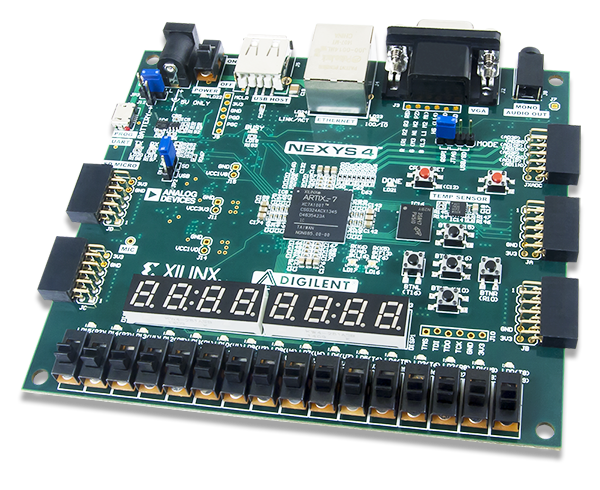
\includegraphics[width=0.3\linewidth]{Images/nexys-4.png}
    \caption{Placa de desenvolupament Nexys4 utilitzada pel desenvolupament d'aquest treball.\cite{NEXYS4Dig}}
    \label{figNEXYS4}
\end{figure}
\chapter{Base Teòrica}
\section{Protocol Inter-Integrated Circuit Sound}
\par El protocol Inter-Integrated Circuit Sound (I2S) és un estàndard de comunicació d'àudio serial que va ser introduït per primer cop l'any 1986 per Philips Semiconductors (ara NXP) i reversionat l'any 1996. L'interfície es va popularitzar amb la implementació en els reproductors de CDs i avui en dia es pot trobar a qualsevol aplicació on es transmeti dades d'àudio digital entre ICs. \cite{I2S_manual}
\par El bus I2S està format per 3 senyals serials:
\begin{itemize}
    \item \textbf{Serial Clock:} és el rellotge que determina la freqüència a la que es transmeten els bits del valor samplejat d'audio.
    \item \textbf{Word Select:} indica el canal que s'està transmetent (esquerra o dret).
    \item \textbf{Serial Data:} per on es transmet la informació bit a bit per canal. 
\end{itemize}
 
\par La informació que es transmet pel Serial Data es fa en complement a 2, essent el bit més significatiu el primer en transmetre's. Existeixen diferents modes d'operació que diferencien el frame que es transmet pel bus I2S.
\begin{itemize}
    \item \textbf{Mode d'Operació Justificat a la Dreta:} També conegut com el format japonès o Sony, aquest estàndard funciona fent que el LSB del canal esquerre es torni vàlid inicialment a la vora ascendent de SCK/BCLK, just abans de la vora descendent del WS. De manera similar, el LSB del canal dret es torna vàlid a la vora ascendent de SCK/BCLK, just abans de la vora ascendent del WS. Un desavantatge del format justificat a la dreta és que el receptor ha de determinar la longitud de paraula de les dades destinades a la transmissió amb antelació.
    \begin{figure}[H]
        \centering
        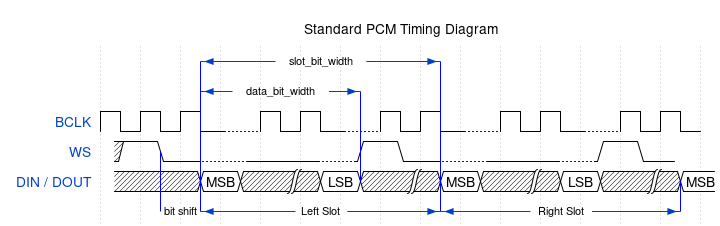
\includegraphics[width=0.7\linewidth]{Images/IS2PCM.png}
        \caption{Frame del bus I2S en mode d'operació justificat a la dreta. \cite{I2SESP32}}
        \label{I2SRightJust_fig}
    \end{figure}
    \item \textbf{Mode d'Operació Justificat a l'Esquerra:} A diferència del format justificat a la dreta, la configuració justificada a l'esquerra elimina qualsevol retard d'un cicle de rellotge relacionat amb BCLK. En aquesta configuració, ambdós canals tenen els seus bits més significatius (MSBs) validats a la primera vora ascendent de BCLK/SCK després de qualsevol modificació del WS. Això contrasta amb l'operació justificada a la dreta, ja que no requereix coneixement previ de la longitud de paraula abans d'iniciar la transmissió.
    \begin{figure}[H]
        \centering
        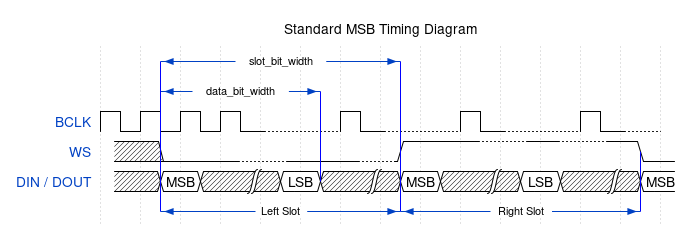
\includegraphics[width=0.7\linewidth]{Images/I2SMSB.png}
        \caption{Frame del bus I2S en mode d'operació justificat a l'esquerra. \cite{I2SESP32}}
        \label{I2SLeftJust_fig}
    \end{figure}
    \item \textbf{Mode d'Operació Estàndard Phillips:} Aquest estàndard es diferencia per un bit de rellotge respecte al format justificat a l'esquerra típic. En aquest cas, s'inicia la transmissió de dades pel Serial Data al segona flanc de pujada del Serial Clock un cop iniciada la transmissió per un canal diferent (canvi de nivell al Word Select).
    \begin{figure}[H]
        \centering
        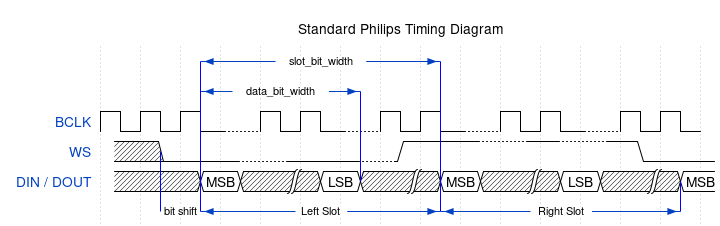
\includegraphics[width=0.7\linewidth]{Images/I2SPhilips.png}
        \caption{Frame del bus I2S en mode d'operació de l'estàndar Philips. \cite{I2SESP32}}
        \label{I2SPhilips_fig}
    \end{figure}
\end{itemize}
\par El Word Select indica el canal que s'està transmetent:
\begin{itemize}
    \item WS = 0: canal 1 (esquerra)
    \item WS = 1: canal 2 (dreta)
\end{itemize}

\par El senyal WS pot canviar tant en una vora descendent com en una vora ascendent del rellotge en sèrie, però no necessita ser simètric. En el dispositiu de destinació, aquest senyal es bloqueja en la vora ascendent del senyal de rellotge. La línia WS canvia un període de rellotge abans que es transmeti el MSB. Això permet que el transmissor de destinació estableixi una temporització síncrona de les dades sèrie que es configuraran per a la transmissió. A més, permet que el receptor emmagatzemi la paraula anterior i buidi l'entrada per a la següent paraula.

\section{Transformada de Fourier}
\par La transformada de Fourier descompon un senyal continu en el temps en un espectre de freqüència que defineix el senyal i per tant, redefineix el senyal en el domini freqüencial. La transformada de Fourier d'un senyal x(t) s'expressa de la següent manera \cite{Bose1985}:
\begin{equation}\label{eqTransFourier}
    X(w) = \int_{-\infty}^{+\infty} x(t)e^{-iwt} \,dt 
\end{equation}

\par I en temps discret, la transformada es redefineix de la següent manera\cite{ImmAudioSign}:
\begin{equation}\label{eqDiscreteFourier}
    X(w) = \sum_{k =-\infty}^{+\infty} x(k)e^{-iwk}
\end{equation}

\section{Teorema de Nyquist}
\par El teorema de Nyquist descriu com samplejar un senyal per evitar que no es perdi informació tot emprant la transformada de Fourier per a representar l'espectre en freqüència del senyal abans i després de ser mostrejada. El teorema diu així \cite{NYQUIST1928}:
\begin{quote}
    \textit{Donat un senyal continu en el temps x(t) limitada en l'ample de banda per fmax, estableix que per poder samplejar el senyal sense perdre informació, cal mostrejar-lo a una freqüència fsample $\geq$ 2fmax. Alternativament, es pot definir la frequencia de Nyquist com: \[f_{nyquist} = \frac{1}{2}f_{sample}\]}
\end{quote}
\par Teòricament, si a un senyal del món real s'aplica el teorema de Nyquist per mostrejar-lo en un sistema discret, és possible reconstruir el senyal original a partir de la freqüència de sampleig. En canvi, si un senyal conté freqüències més enllà de l'ample de banda considerat per al mostreig d'aquest senyal, el sistema resulta submostrejat i no serà possible reconstruir el senyal original. Per evitar situacions on la pèrdua sigui notòria i pugui perjudicar el processament d'aquests senyals, típicament els senyals es sobremostregen a freqüències més altes del doble de la freqüència mes alta en tot l'espectre del senyal a mostrejar.
\par No obstant, en la conversió dels senyals continus a temps discret, si s'omet part del seu espectre frequencial, dona lloc a l'efecte de l'aliàsing. Aquest efecte apareix com la superposició de les imatges a freqüències més altes del senyal sobre l'espectre mostrejat, entenent imatge com l'ample de banda del senyal que comprén: \[Nf_{sample} + 1 \leq f < (N+1)f_{sample}\] En el món pràctic, no existeixen senyals pures i la majoria tenen components de freqüència extremadament alta més enllà de la freqüència de Nyquist. 

\begin{figure}[H]
    \centering
    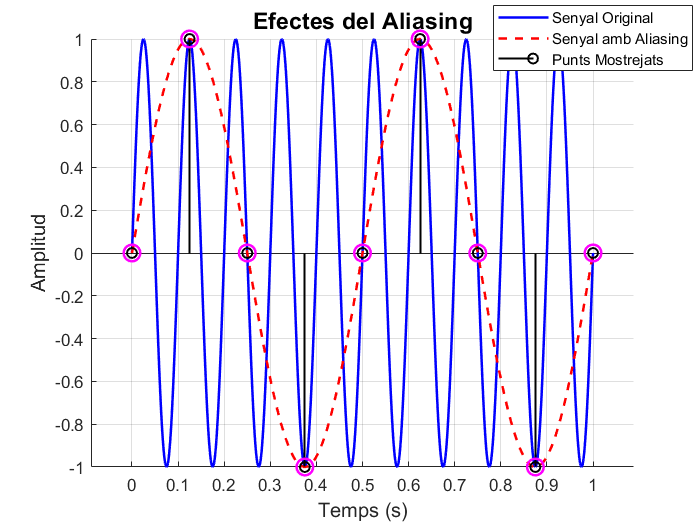
\includegraphics[width=0.5\linewidth]{Images/imatge_aliasing.png}
    \caption{Efectes de l'Aliasing en un senyal sinusoidal on la freqüència de mostreig es superior a la freqüència de Nyquist}
    \label{Aliasing_fig}
\end{figure}

\section{Transformada en \textit{z}}
\par La transformada en z es una generalització de la transformada de Fourier, que es pot expressar com les sèries de Laurent amb la variable complexa z = exp(jw). Donada una seqüència x[n], la corresponent transformada en z es defineix com\cite{ImmAudioSign}:
\begin{equation}\label{trans_z}
    X(z) =  \sum_{n=0}^\infty x(n)z^{-n}
\end{equation}
\par Un dels motius per utilitzar la transformada en z és que la transformada de Fourier no convergeix per tots els senyals en temps discret i és útil tenir una generalització de la transformada de Fourier que englobi una classe més àmplia de senyals.
\par Com es pot apreciar observant les equacions \ref{eqDiscreteFourier} i \ref{trans_z}, existeix una relació directa entre la transformada de Fourier i la transformada en \textit{z}. Aquesta relació es pot constatar substituint la variable z en l'equació \ref{trans_z} per la variable complexa exp(jw), aleshores la transformada en z es redueix a la transformada de Fourier. Aquest és un dels motius pels quals s'empra la notació de la transformada de Fourier en termes de exp(jw), doncs facilita el canvi de domini de temps discret a freqüencial \cite{DiscreteTimeSP}. Això es correspon a una restricció de la variable z amb magnitud unitària. De manera més genèrica és possible expressar la variable z en forma polar com: \[z = re^{jw}\] Amb aquesta última expressió de z, si es substitueix a \ref{trans_z} es converteix en l'equació \ref{eqDiscreteFourier}.

\par En el pla z, el contorn que es correspon amb abs(z) = 1 és un cercle de radi la unitat, també referit com el cercle unitari. La transformada en z estudiada dins d'aquest cercle es correspon a la transformada de Fourier. En el pla polar z, l'angle que forma el vector que apunta a un punt z dins el cercle unitari es correspon a la pulsació w en rad/s. I doncs, si s'evaluessin els punts en el cercle unitari per w = 0 a w = 2$\pi$, es correspondria a examinar la transformada de Fourier en l'espectre de freqüències de 0 a 2$\pi$. Aquesta interpretació equival conceptualment a embolicar l'eix de freqüència de la transformada de Fourier al voltant del cercle unitari.

\section{Processament Digital de Senyals}
\subsection{Senyals en temps discret}
\par Els senyals en temps discret es representen matemàticament com seqüències de números, on l'n-èssim número s'indica com x[n].
\par En els senyals de temps discret, els valors del senyal es representen en intèrvals discrets i com seqüències de números, on l'n-èssim número s'indica com x[n] o x[nTs]. Ts representa el període de mostreig i defineix l'interval de temps en que es prenen els valors d'un senyal continu. 
\par En l'estudi dels senyals i sistemes en temps discret, apareixen sovint un seguit de senyals que juguen un paper important. Aquestes són \cite{DiscreteTimeSP}:
\begin{itemize}
    \item impuls unitari: La sequència que defineix aquest senyal es caracteritza per ser 1 en n = 0 i 0 en qualsevol altre instant. 
    \begin{equation}\label{delta_unit}
        \delta(n) = \left\lbrace\begin{array}{c} 1\quad n = 0 \\ 0\quad n \neq 0 \end{array}\right.
    \end{equation}
    \begin{figure}[H]
        \centering
        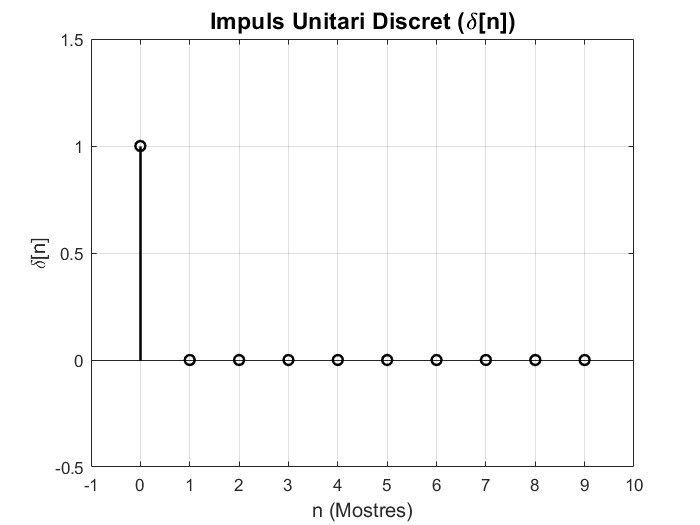
\includegraphics[width=0.5\linewidth]{Images/imatge_delta.png}
        \caption{Impuls unitari en temps discret de n = 10 mostres.}
        \label{delta_imp_fig}
    \end{figure}
    \item esglaó unitari: aquest senyal té valor zero pels instants abans de zero i pren valor unitari en l'instant zero i posteriors.
    \begin{equation}\label{step_unit}
        u(n) = \left\lbrace\begin{array}{c} 1\quad n \geq 0 \\ 0\quad n < 0 \end{array}\right.
    \end{equation}
    \begin{figure}[H]
        \centering
        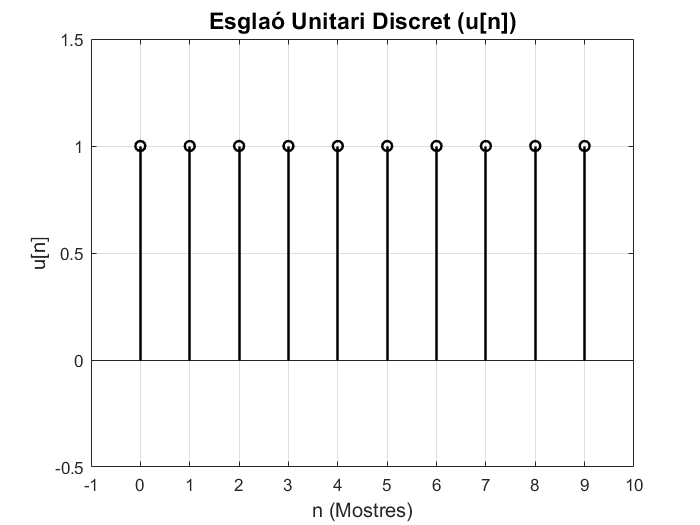
\includegraphics[width=0.5\linewidth]{Images/imatge_esglao.png}
        \caption{Esglaó unitari en temps discret de n = 10 mostres.}
        \label{step_fig}
    \end{figure}
    \item rampa discretitzada: per instants previs a zero pren valor zero, i a partir de l'instant zero pren el n-èssim valor que representa.
    \begin{equation}\label{ramp_func}
        u(n) = \left\lbrace\begin{array}{c} n\quad n \geq 0 \\ 0\quad n < 0 \end{array}\right.
    \end{equation}
    \begin{figure}[H]
        \centering
        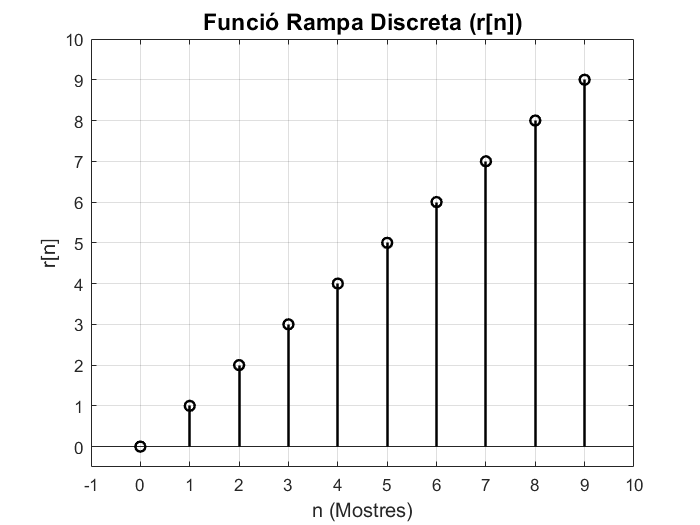
\includegraphics[width=0.5\linewidth]{Images/imatge_rampa.png}
        \caption{Funció rampa en temps discret de n = 10 mostres.}
        \label{ramp_fig}
    \end{figure}    
\end{itemize}

\par En el domini digital, els senyals només es poden representar en un rang de nombres enters i en la conversió de temps continu a temps discret és necessari aplicar un procés de requantificació. Aquesta transformació insereix soroll inevitablement al senyal, que mitjançant tècniques de processament digital és possible mitigar. Aquest soroll és complicat de descriure matemàticament doncs no és exactament lineal ni previsible en sistemes complexos de processament de senyals. No obstant, existeixen tècniques de modulació de soroll que mitiguen aquest fenomen d'acoplament de senyals indesitjat i que més endavant en aquest treball es comentaran breument.
\subsection{Sistemes en temps discret}
\subsubsection{Sistemes Lineals}
\par Les operacions realitzades per un sistema de processament digital es basen en la premissa que el sistema satisfà les propietats de linearitat i invariància en el temps. Si considerem un sistema lineal, les transformacions que aquest sistema realitza compleixen les propietats d'homogeneïtat, additivitat i de superposició \cite{DiscreteTimeSP}. A continuació es poden observar les demostracions:
\begin{itemize}
    \item Additivitat: Donat un sistema \textit{S} que a una entrada $x_1$ obté a la sortida $y_1$ i que a una entrada $x_2$ respon amb $y_2$, el sistema compleix la propietat d'additivitat si es satisfà:
    \begin{equation}\label{additivity_eq}
        S(x_1 + x_2) = y_1 + y_2
    \end{equation}
    \item Homogeneitat: Donat un sistema \textit{S} que a una entrada $x_1$ obté a la sortida $y_1$, el sistema compleix la propietat d'homogeneitat si es satisfà:
    \begin{equation}\label{homogeneity_eq}
        S(ax_1) = ay_1
    \end{equation}
    \item Superposició: Si un sistema \textit{S} es considera lineal i compleix les propietats d'homogeneitat i linealitat, per necessitat compleix la propietat de superposició. La demostració de la propietat de superposició d'un sistema \textit{S}, s'expressa de la següent forma:
    \begin{equation}
        S(ax_1+ax_2) = ay_1 + ay_2
    \end{equation}
\end{itemize}


\subsubsection{Sistemes de Temps Invariant}
\par  Un sistema invariant en el temps és aquell per al qual una entrada retardada de n mostres resulta en una sortida retardada de n mostres. Específicament, si considerem un sistema \textit{S}, per una entrada retardada k mostres es considera que el sistema és invariant en el temps si:  
\begin{equation}
    S(x(n-k)) = y(n-k)
\end{equation}

\subsubsection{Sistemes de Temps Invariant i Lineals}
\par Els sistemes lineals i de temps invariant tenen aplicacions rellevants en el processament digital de senyals degut que les propietats d'aquests sistemes estan definides per les de la convolució en temps discret. 

\par Aquests sistemes tenen la propietat que essent y(n) la resposta a la seqüència d'entrada x(n), la resposta a la seqüència desplaçada x(n-k) és y(n-k), que és la mateixa resposta que a la seqüència x(n), desplaçada per la mateixa quantitat k. A causa d'aquesta propietat, es pot demostrar immediatament que si un sistema és lineal i invariant en el temps, es pot caracteritzar per la seva resposta a un impuls unitari. Per als sistemes lineals invariants en el temps, l'expressió genèrica que els defineix ve donada per:
\begin{equation}\label{eq_summ_lti}
    y[n] = \sum_{k=-\infty}^{\infty} x[k]h_k[n] 
\end{equation}
\par L'equació \ref{eq_summ_lti} també es coneix com convolució i demostra que un cop es coneix h(n), és possible determinar la resposta a qualsevol altra seqüència d'entrada x(n). \cite{DiscreteTimeSP} 

\section{Filtres Digitals}
\subsection{Filtres FIR}
\par De la traducció literal de la seva denominació anglosaxona, els filtres FIR són filtres amb una \textit{Resposta d'Impuls Finit}, altrament referits com filtres de mitjana mòbil, filtres transversals o, en referència a la naturalesa de la seva implementació, filtres no recursius. En el processament digital de senyals d'àudio, són la topologia de filtres més populars degut a la baixa complexitat en la implementació i la linealitat en la seva resposta en fase.
\par Els filtres FIR posseeixen certes característiques desitjables, per definició són sistemes de tipus Lineal i Invariant al Temps és a dir, com s'ha comentat a l'apartat de sistemes Lineals i de Temps Invariant, compleixen les propietats de superposició, homogeneïtat i invariança. Conseqüentment, tenen un seguit de ventatges en l'espectre freqüencial com el desfassament lineal, l'estabilitat inherent i la baixa sensibilitat als errors de quantificació \cite{DigitalSignalPr}. La resposta d'un filtre de longitud L o ordre N = L - 1, ve donada per la convolució de les mostres actuals i anteriors a l'entrada del filtre, i els coeficients del mateix. I la funció de transferència en el domini \textit{z} ve definida per:
\begin{equation}\label{eq_FIR}
    H(z) = \sum_{k=-\infty}^{\infty} h_k z^{-n}
\end{equation}
\par Els coeficients $h_k$ defineixen els zeros del filtre caracteritzant la resposta en freqüència. La presència de només zeros al polinomi \ref{eq_FIR} confirma la teòrica estabilitat dels filtres FIR.
\begin{figure}[H]
    \centering
    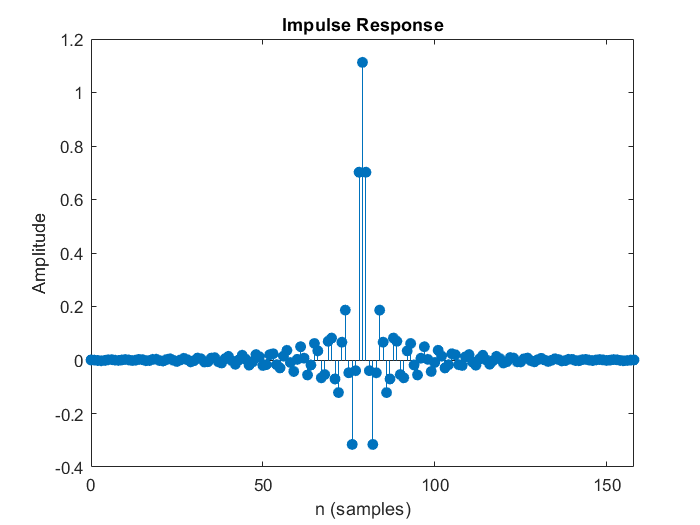
\includegraphics[width=0.5\linewidth]{Images/FIRimpulse.png}
    \caption{Resposta a un impuls unitari d'un filtre FIR}
    \label{figFIRimpulse}
\end{figure}

\subsubsection{Filtres CIC}
\par En el processament de senyals digitals, un Cascaded Integrator-Comb (CIC) és una classe computacionalment eficient de filtres FIR passa-baixos, que encadena N nombre de parells integradors i filtres de pinta (on N és l'ordre del filtre) per formar un decimador o interpolador. Els filtres de pinta són blocs que s'utilitzen en el processament digital de senyals en realitzar la suma d'una mostra retardada amb l'actual \cite{CICLyons}. 
\begin{figure}[H]
    \centering
    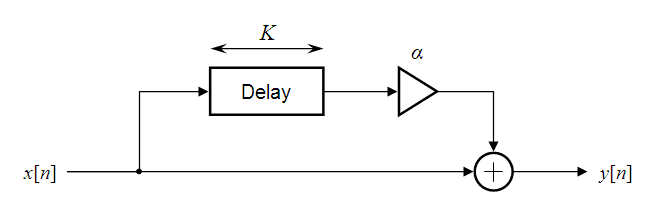
\includegraphics[width=0.5\linewidth]{Images/Comb_filter_feedforward.png}
    \caption{Bloc de filtrat Comb o de pinta. \cite{CICLyons}}
    \label{figComb}
\end{figure}
\par Els filtres CIC s'originen a partir de la reestructuració dels interpoladors de mitjana mòbil com el de la figura \ref{figMAFilter}. A partir de la equació \ref{eqMovAv}, es pot intuir que els blocs CIC mantenen la propietat d'interpolació amb l'afegit que la resposta en freqüència es veu modificada per la presència dels blocs integradors i Comb. Més específicament, modificant els blocs Comb es situen els zeros i amb els blocs integradors els pols de la funció de trasferència. 
\begin{figure}[H]
    \centering
    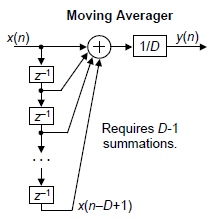
\includegraphics[width=0.3\linewidth]{Images/fir-mvavg-form.png}
    \caption{Diagrama de blocs d'un filtre de mitjana mòbil.}
    \label{figMAFilter}
\end{figure}

\begin{equation}\label{eqMovAv}
    y[n] = x[n] + x[n-1] + x[n-2] + x[n-3] \longrightarrow y[n] = y[n-1] + x[n] + x[n-4]
\end{equation}

\par En un CIC de delmat, el senyal d'entrada passa primer per N etapes integradores, seguides d'un procés de mostreig descendent, i finalment per N etapes de diferència (etapes de Comb). D'altra banda, un CIC interpolador segueix l'ordre invers d'aquesta arquitectura: primer aplica N etapes de Combs, seguit del zero stuffing i, finalment, N etapes integradores \cite{Hogenauer1981}.
\begin{figure}[H]
    \centering
    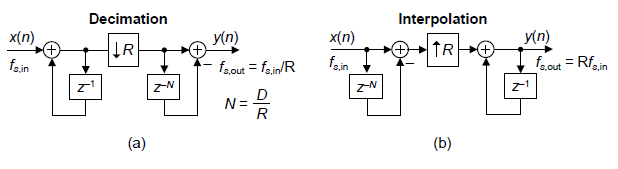
\includegraphics[width=0.7\linewidth]{Images/CIC_digital_filters.png}
    \caption{Implementacions de filtres CIC en una sola etapa: (a) Delmat; (b) Interpolació \cite{CICLyons}}
    \label{figCICDeciInt}
\end{figure}
\newpage
\subsection{Filtres IIR}
\par La resposta a un impuls unitari d'aquests filtres és una seqüència infinita, fet que dona lloc a la seva denominació com a filtres IIR (\textit{Infinite Impulse Response}). Típicament, aquests filtres requereixen menys recursos i poden executar tasques de filtratge a major velocitat que els filtres FIR. 
\par En un filtre IIR implementat de manera recursiva, la mostra de sortida y(k) és una combinació lineal de les mostres d’entrada actuals i passades de la seqüència x(k), així com de les mostres de sortida passades. Aquesta estructura recursiva és la clau per obtenir una alta eficiència i permet que els filtres IIR es comportin com una aproximació dels sistemes analògics \cite{Bose1985}.
\par Un filtre IIR no és útil si no és estable. Per tant, cal fer comprovacions d'estabilitat en tots els dissenys, i si es detecta que un filtre és inestable, s’han de proporcionar esquemes satisfactoris d'estabilització. En moltes aplicacions, on es busca la linealitat de la característica de fase com en el tractament de senyals d'àudio, un filtre IIR sol ser poc pràctic\cite{DigitalSignalPr}.
\par Comparat amb un filtre FIR, un filtre IIR sovint pot ser molt més eficient en termes d'assolir certes característiques de rendiment amb un ordre de filtre determinat. Això es deu al fet que el filtre IIR incorpora retroalimentació i és capaç de realitzar tant els zeros com els pols d'una funció de transferència del sistema, mentre que el filtre FIR és un filtre només de zeros. Però, per contrapartida, els filtres IIR són més sensibles a la quantificació dels coeficients i poden derivar en inestables si la requantificació no es fa correctament. A l'equació \ref{eqIIR} s'expressa la funció de transferència general dels filtres IIR.
\begin{equation}\label{eqIIR}
    H_{IIR}(z) = \frac{\sum_{k=0}^{M} b_k z^{-k}}{\sum_{k=0}^{M} a_k z^{-k}}
\end{equation}

\section{Modulador $\Sigma \Delta$}
\par Els moduladors $\Sigma \Delta$ o $\Delta \Sigma$ son una topologia de convertidors ADC o DAC molt popular per la seva propietat de modelat del soroll de quantificació. 
\par La tècnica de modulació sigma-delta és la tecnologia més popular en convertidors d'àudio A/D i D/A dels últims 30 anys, gràcies al modelat de soroll característic de la seva estructura. La nomenclatura utilitzada per descriure aquest tipus de modulació reflecteix les seves propietats tècniques i explica per què és especialment atractiva per a la implementació en convertidors tant A/D com D/A.
\par La lletra $\Delta$ prové de l'alfabet grec i, en el context matemàtic, s'utilitza habitualment per representar variacions o diferències d'una magnitud. En la tècnica de modulació sigma-delta, $\Delta$ fa referència al càlcul de la diferència entre la mostra d'entrada i la sortida anterior quantitzada.

\par D'altra banda, la lletra $\Sigma$, també originària de l'alfabet grec, s'empra sovint per representar processos de suma. En el cas del modulador en qüestió, aquesta suma correspon a una integral en temps discret. L'efecte d'aquest bloc integrador és el que fa que la tècnica de modulació sigma-delta sigui tan interessant per a aplicacions amb requeriments exigents pel que fa al SNR del senyal. Aquest bloc es tractarà amb més detall més endavant. 
\par Essencialment, un convertidor $\Sigma \Delta$ digitalitza el senyal d'entrada amb baixa resolució (típicament d'1 bit però es poden implementar estructures amb més nivells segons el quantificador a la sortida) a una freqüència de mostreig alta. L'efecte del sobremostreig distribueix el soroll de quantificació en un espectre de freqüència més ampli que el del senyal d'interès. L'altre fenomen interessant del modulador és l'atenuació del soroll de quantificació, ja que el bloc es comporta com un filtre passa-alts per l'error en el procés de quantificació, provocant que la major part de la potència del soroll no desitjat es situï més enllà de l'amplada de banda del senyal d'interès. Per tant, en el modulador $\Sigma \Delta$ l'efecte del sobremostreig juntament amb la modulació del soroll de quantificació permeten millorar el SNR del senyal d'entrada i obtenir alts rendiments a baix cost computacional. Addicionalment, el senyal que conté la informació d'interès no es veu modificat. 
\par L'estructura més bàsica de les topologies $\Sigma \Delta$ permet entendre les propietats dels moduladors derivats d'aquesta família. A partir del sistema representat a la figura \ref{figMOD1}, que mostra un modulador $\Sigma \Delta$ de primer ordre amb realimentació negativa, es pot descriure el seu comportament mitjançant l'equació \ref{eqMOD1}.
\begin{figure}[H]
    \centering
    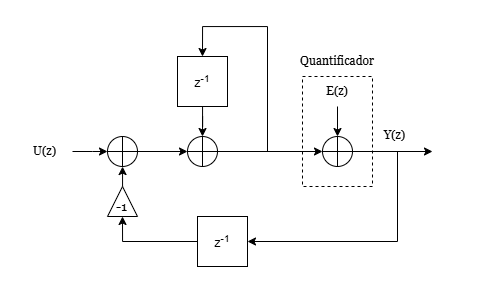
\includegraphics[width=0.5\linewidth]{Images/SigmaDeltaMOD1.drawio.png}
    \caption{Modulador $\Sigma \Delta$ de primer ordre.}
    \label{figMOD1}
\end{figure}
\begin{equation}\label{eqMOD1}
    Y(z) = 1 \ U(z) + (1 - z^{-1})E(z)
\end{equation}
\par A partir de l'equació \ref{eqMOD1}, es pot observar que el senyal d'entrada U(z) no es veu afectada pel sistema implementat, mentre l'error de quantificació està modelat per un filtre passa alts de primer ordre (1 - $z^{-1}$). A la figura \ref{fig_NTFpendent} es pot apreciar el comportament del modelat del soroll de quantificació del sistema, amb una pendent de la banda de transició de 20 dB/dec. 
\begin{figure}[H]
    \centering
    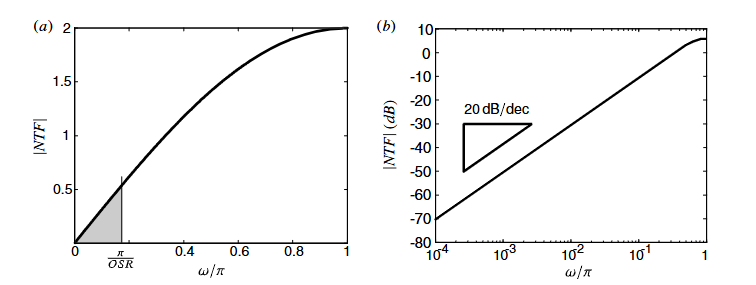
\includegraphics[width=0.6\linewidth]{Images/graficaNTFMOD1.png}
    \caption{Resposta en freqüència de NTF(z) d'un modulador $\Sigma \Delta$ de primer ordre. \cite{UndrstndSDM}}
    \label{fig_NTFpendent}
\end{figure}

\par L'ús d'integradors permet que la funció de transferència del senyal (STF) mantingui un guany unitari, mentre que el soroll de quantificació es redueix significativament a la banda de freqüència d'interès. Aquest enfocament permet aconseguir un SNR o SNDR més elevat segons els requisits del sistema. No obstant, l'addició de més etapes integradores no es pot fer manera directa ja que presenta problemes d'estabilitat. Degut a que cada etapa afegeix un canvi de fase de 90º, l'ordre del filtre de retroalimentació no pot ser més gran de 2. 

\subsubsection{Topologies de moduladors $\Sigma \Delta$}
\par A banda de l'estructura fonamental dels moduladors $\Sigma \Delta$ com el de la figura \ref{figMOD1}, existeixen diverses topologies que s'han desarollat per poder afrontar requeriments més exigents que els assumibles per un modulador de primer ordre. A continuació es comentaran breument les més rellevants \cite{SDMToolbox}:
\begin{itemize}
    \item \textbf{CIFB}: Els coeficients $a_n$ ubiquen els pols del NTF i el STF, mentre que els coeficients $b_n$ mapejen els zeros del STF. Els coeficients de les variables d'estat $c_n$ s'utilitzen per escalar el rang dinàmic.
    \begin{figure}[H]
        \centering
        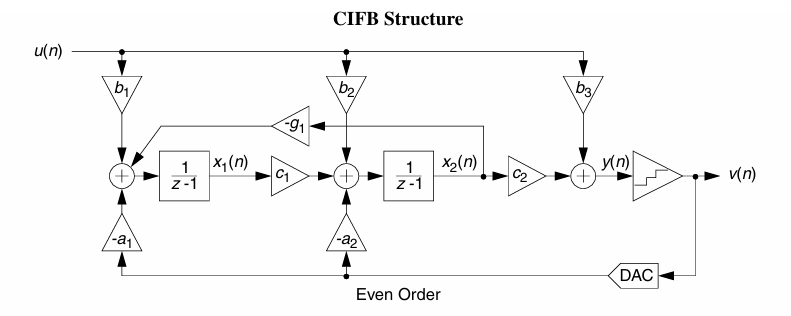
\includegraphics[width=0.5\linewidth]{Images/CIFB.png}
        \caption{Modulador $\Sigma \Delta$ CIFB}
        \label{figCIFB}
    \end{figure}
    \item \textbf{CRFB}: L'estructura és similar als CIFB a diferència del ressonador estable que es forma amb la implementació d'un bloc integrador amb delay i un bloc integrador sense i el llaç de realimentació creat amb $g_n$.
    \begin{figure}[H]
        \centering
        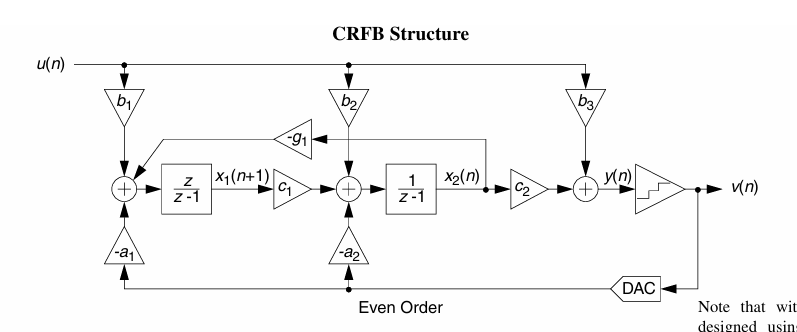
\includegraphics[width=0.5\linewidth]{Images/CRFB.png}
        \caption{Modulador $\Sigma \Delta$ CRFB}
        \label{figCRFB}
    \end{figure}
    \item \textbf{CIFF}: A la sortida es calcula la suma de les variables d'estat. El llaç de realimentació mitiga el soroll de quantificació.
    \begin{figure}[H]
        \centering
        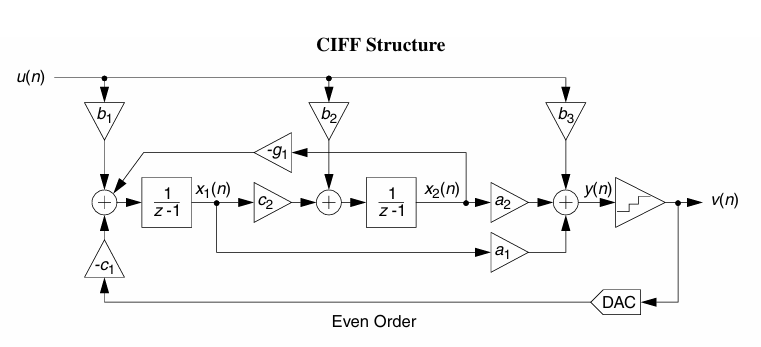
\includegraphics[width=0.5\linewidth]{Images/CIFF.png}
        \caption{Modulador $\Sigma \Delta$ CIFF}
        \label{figCIFF}
    \end{figure}
    \item \textbf{CRFF}: S'implementa l'estructura CIFF amb resonadors que afegeixen zeros complexes en NTF.
    \begin{figure}[H]
        \centering
        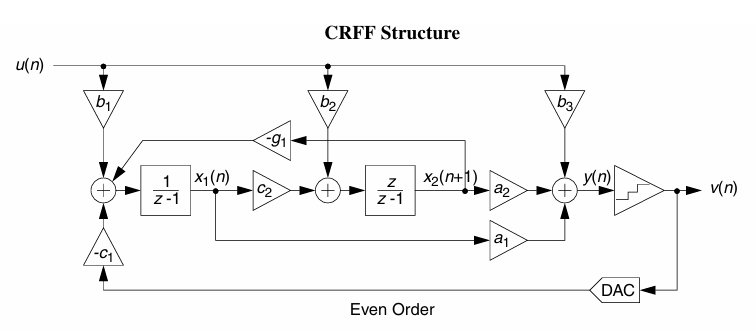
\includegraphics[width=0.5\linewidth]{Images/CRFF.png}
        \caption{Modulador $\Sigma \Delta$ CRFF}
        \label{figCRFF}
    \end{figure}
\end{itemize}
\section{PWM}
\par La modulació per amplada de pols (PWM) és una tècnica de control utilitzada en convertidors d'electrònica de potència per regular l'alimentació subministrada des de la font d'alimentació fins a la càrrega. En un senyal PWM, la freqüència del cicle de generació de polsos és un paràmetre fix i l'amplitud d'aquests polsos, una variable. D'aquesta forma, modificant l'amplitud dels polsos s'obté el valor promig a la càrrega equivalent al senyal original sense modular. Aquesta generació del senyal PWM es pot fer en domini analògic o en domini digital. En el domini analògic, els circuits amb amplificadors operacionals s'utilitzen àmpliament per generar PWM a partir de senyals portadores i modulants. Però aquests circuits són més susceptibles a les derives de la temperatura i a la degradació amb el pas del temps dels components que en conjunt acaben oferint un rendiment pitjor del sistema original. En el medi analògic, les entrades del modulador d'ample de banda són el senyal analògic a modular i una ona triangular com a tensió de referència per calcular l'amplitud dels polsos a la sortida. Anàlogament, en el medi digital s'aconsegueix un efecte similar i la implementació d'algorismes avançats és relativament fàcil i més ràpida. \cite{PWMarticle} 
\begin{figure}[H]
    \centering
    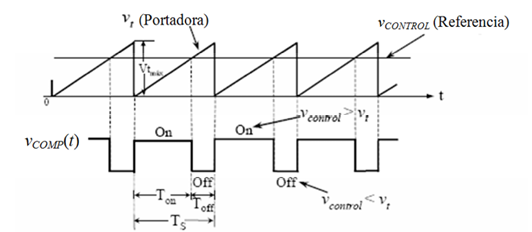
\includegraphics[width=0.5\linewidth]{Images/PWM_Pique.png}
    \caption{Frame dels senyals implicats en el procés de modulació per ample de polsos en el medi analògic, on el senyal de control representa l'amplitud a transmetre a la sortida. \cite{PiquePWR}}
    \label{PWM_analog_fig}
\end{figure}
\par Com es pot observar a la imatge \ref{PWM_analog_fig}, el temps que el senyal de sortida del modulador està a nivell alt és directament proporcional a la relació entre l'amplada del senyal de control i el del portador. Aquesta relació també es coneix com \textit{duty cycle} que es representa matemàticament de la següent forma:
\begin{equation}\label{duty_eq}
    \delta(t) = \frac{V_{control}(t)}{V_{t,max}(t)}
\end{equation}
On Vcontrol és el valor del senyal a modular i Emax, la tensió màxima del senyal triangular o portador.

\section{Mètriques de rendiment}

\subsection{SNR}
\par El Signal to Noise Ratio (SNR) ve donat per la relació entre la potència del senyal i la potència del soroll, per a una certa amplitud d'entrada. No té en compte els components del senyal harmònicament relacionats \cite{ADC16b}.
\begin{equation}\label{SNR_eq}
    SNR(dB) = 20log_{10}(\frac{P_{Senyal}}{P_{Soroll}})
\end{equation}
\par En el context del processament digital de senyals, sovint es menciona aquest mesura com SQNR (Signal to Quantization Noise Ratio) doncs en el domini digital es d'interès coneixer la capacitat d'un procés de mitigar el soroll provocat per la quantificació del senyal mostrejat. De \cite{UndrstndSDM}, s'obté que l'expressió del SQNR(dB) és:
\begin{equation}\label{eq_SQNR}
    SQNR(dB) = 10log_{10}(\frac{15 M^2 (OSR)^5}{2\pi^4})    
\end{equation}
on M és els nombre de nivells del quantificador.
\par De forma similar, el Signal to Noise and Distortion Ratio (SNDR) és la relació entre la potència del senyal i el soroll i tots els components de potència de distorsió. Així, té en compte diversos dels harmònics (típicament el 2n i el 3r harmònic) que es troben dins de la banda d'interès. \cite{SDMClassD}

\subsection{DR}
\par El Dynamic Ratio (DR) és el rang d'amplituds del senyal sobre el qual l'estructura funciona correctament, és a dir, dins dels límits acceptables de distorsió. Està determinat pel senyal d'entrada d'amplitud màxima i pel senyal d'entrada detectable més petit. \cite{ADC16b}
\begin{equation}
    DR(dB) = 10log_10(\frac{3(2^{B}-1)^{2}(2L+1)OSR^{2L +1}}{2\pi^{2L}}
\end{equation}

\subsection{THD}
\par La distorsió harmònica total és la relació entre la suma de la potència del senyal de totes les freqüències harmòniques per sobre de la freqüència fonamental i la potència de la freqüència fonamental. La distorsió harmònica generada per un n-èsim harmònic específic també es pot determinar i està donada per la relació entre la potència del senyal i la potència del component de distorsió en aquest n-èsim harmònic de la freqüència del senyal \cite{PiquePWR}.
\begin{equation}
    THD = \frac{\sqrt{V_{n+1}^{2}+V_{n+2}^{2}+V_{n+3}^{2}+...}}{V_{n}^{2}}
\end{equation}

\subsection{Soroll de Quantificació}
\par El procés de quantificació inevitablement introdueix distorsió en la senyal degut a que en la conversió d'un senyal continu al domini digital es perd informació. Aquest procés té una característica d'escala i la diferència entre dos valors quantificats adjacents s'anomena mida de pas ($\Delta$). Per a valors d'entrada grans, la sortida del quantificador pot arribar a saturar. L'interval de conversió pel qual el quantificador no desborda, s'anomena interval d'escala completa (FS) del quantitzador. Un quantitzador amb un nombre de bits N, pot representar fins a 2N nivells d'amplitud, donant com a resultat un $\Delta$ donat per:
\begin{equation}\label{eq_stepsize}
    \Delta = \frac{FS}{N}
\end{equation}
\par En el procés de quantificació, totes les entrades s'arrodoneixen al nivell més pròxim fet que implica que l'error induït pel procés es troba en el rang [$-\frac{\Delta}{2}$, $\frac{\Delta}{2}$]. Si es considera que la distribució d'aquest error és uniforme en tot el rang d'aparició, la potència mitjana és:
\begin{equation}\label{eq_pwrquant}
    P_{q_{e}}\ = \frac{1}{\Delta} \int_{-\frac{\Delta}{2}}^{\frac{\Delta}{2}} q_{e}^2 \ d q_{e} = \frac{\Delta^2}{12}
\end{equation}
\par Com més gran sigui la resolució del quantificador, més petit és $\Delta$. Així, augmentant el nombre de bits (N) del quantitzador, la potència mitjana del soroll disminueix. 
\par Quan es mostreja un senyal a una freqüència $f_s$, la distribució del soroll de quantificació és uniforme al llarg del rang de freqüències [$-\frac{f_s}{2}$, $\frac{f_s}{2}$]. Per tant, la distribució de la potència del soroll espectral ve donada per: 
\begin{equation}\label{eq_energy_quant}
    E(f) = \frac{\Delta^2}{12 f_s}
\end{equation}
\par De l'equació \ref{eq_energy_quant} es dedueix que, amb una major freqüència de mostreig, l'error de quantificació es redistribueix en un espectre més ampli, reduint així la densitat espectral d'aquest error. Per tant, el procés de sobremostreig contribueix a disminuir l'impacte de l'error de quantificació en la banda de freqüències d'interès.

\chapter{Proposta de resolució}
\section{Diagrama de blocs del sistema}
\par En aquest apartat es presenta el sistema que s'implementarà en aquest treball, i s'exposen les diverses funcionalitats de cada bloc. A la figura \ref{figTFGDiagr} es pot observar el diagrama de blocs del treball.

\begin{figure}
    \centering
    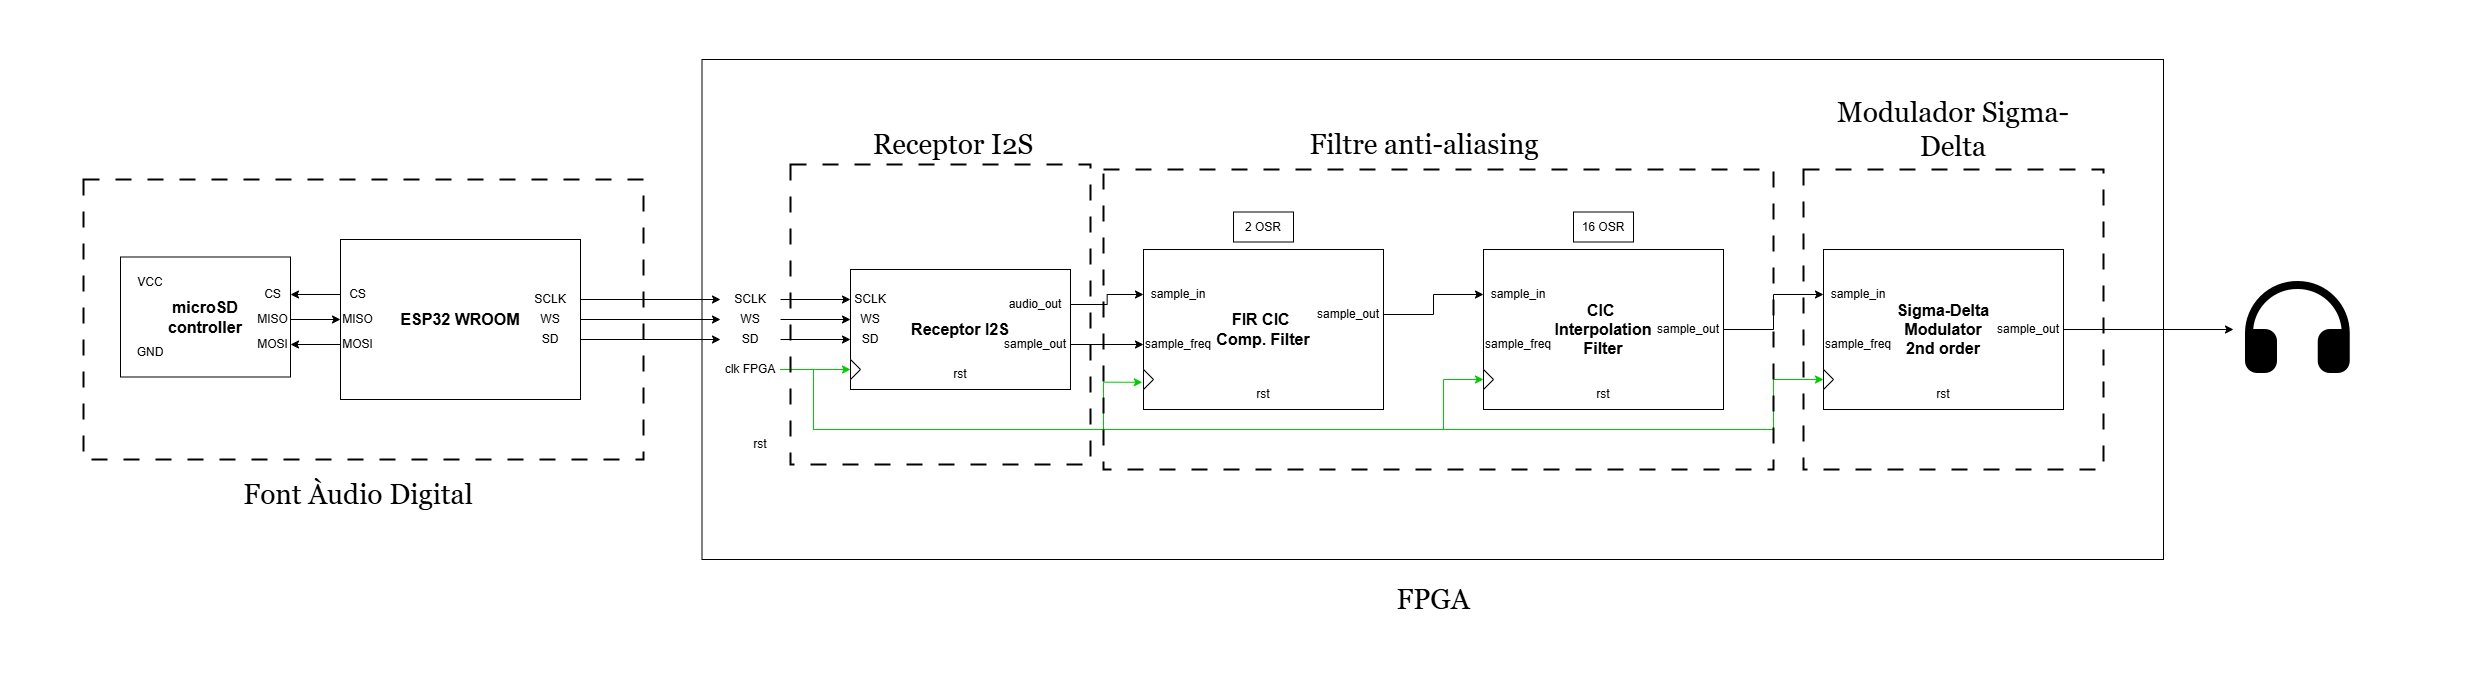
\includegraphics[angle=90,origin=c, width=0.4\linewidth]{Images/EstatActualTFG.drawio.png}
    \caption{Diagrama de blocs del sistema implementat en aquest treball.}
    \label{figTFGDiagr}
\end{figure}

\section{Font d'àudio en protocol I2S}
\par Per poder validar el funcionament de l'amplificador digital cal tenir una font d'àudio que transmeti en protocol I2S. Degut a que aquest protocol s'utilitza en comunicacions entre ICs, s'ha hagut d'implementar una entrada d'àudio que mantingui el protocol amb una targeta externa a la placa de desenvolupament. S'ha utilitzat una $\mu$SD per emmagatzemar els archius d'àudio .wav.

\section{Receptor d'àudio en protocol I2S}
\par S'ha implementat una entitat receptora en protocol I2S per captar les trames que s'envien pel bus. Aquest bloc és la primera etapa en el sistema implementat a la FPGA, i transmet el senyal internament a l'etapa de filtre anti-aliasing. El bloc està configurat per captar trames en mode d'operació estàndard Philips (veure apartat Protocol Inter-Integrated Sound).

\section{Etapa de filtrat anti-aliasing}
\par Com s'estudiarà més endavant, el filtre anti-aliasing s'implementa amb l'objectiu de mitigar l'acoblament d'imatges de freqüències més altes que la de mostreig, a l'espectre d'interés del senyal. En aquest treball es realitza l'etapa de filtrat en dos sub-blocs per efectuar l'etapa de sobre-mostreig de forma que no afecti a la qualitat del senyal.

\section{Modulador $\Sigma\Delta$}
\par L'última etapa de l'amplificador digital d'àudio de classe D desenvolupat en aquest treball és la del modelat de soroll. En el present treball la modelació del soroll de quantificació es realitza amb un bloc $\Sigma\Delta$ de segon ordre. 
\chapter{Entrada d'Àudio Digital}
\section{Font d'àudio digital}
\par Per transmetre a l'entrada de l'amplificador un senyal d'àudio en protocol I2S, s'ha emprat una targeta ESP32-WROOM-32 juntament amb un lector de targetes microSD controlat per SPI. 
 \par El tamany de la memòria RAM de l'ESP32 és de 520 kBytes i per reproduir arxius d'àudio com el d'una cançó es necessiten de l'ordre de MBytes; és per això que per emmagatzemar arxius de major tamany, s'ha utilitzat el mòdul adaptador de targetes microSD, per poder fer la lectura del contingut mitjançant el protocol SPI.
 \par Per implementar la font d'àudio, s'han emprat els següents dispositius i components:
 \begin{itemize}
     \item \textbf{Targeta ESP32-WROOM-32:} Aquesta targeta inclou el MCU encarregat de llegir la targeta microSD i transmetre la informació pel bus I2S.
     \begin{figure}[H]
         \centering
         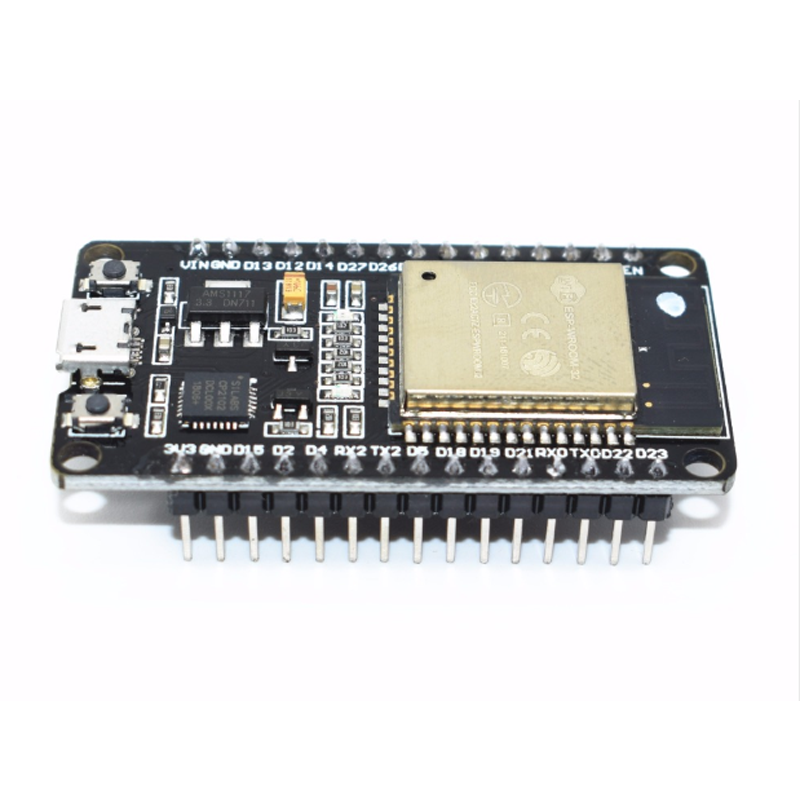
\includegraphics[width=0.25\linewidth]{Images/wroom-32-v2.jpg}
         \caption{Targeta MCU del ESP32-WROOM-V2.}
         \label{ESP32_fig}
     \end{figure}
     \item \textbf{Mòdul adaptador de la targeta microSD:} Aquest mòdul està pensat per poder utilitzar-lo amb tota la gamma de productes d'Arduino, per això a més del suport per a la targeta microSD, inclou un LDO de 3V3 i un Level-shifter que en cas d'utilitzar una placa Arduino amb lògica de 5 V, no faci malbé la targeta.
     \begin{figure}[H]
         \centering
         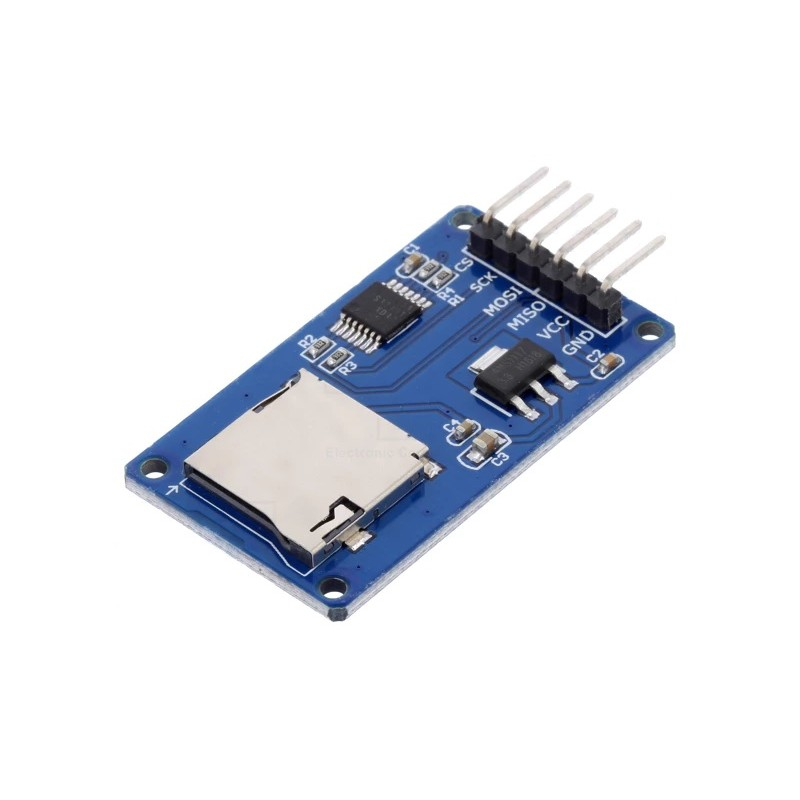
\includegraphics[width=0.25\linewidth]{Images/microsd_arduino.jpg}
         \caption{Adaptador de targeta microSD a SPI.}
         \label{microSD_adapter_fig}
     \end{figure}
     \item \textbf{Mòdul d'alimentació 5 V:} Per poder comunicar-se amb la targeta microSD, com s'ha mencionat en l'anterior ítem, el mòdul adaptador de la targeta microSD ha d'estar alimentat a 5 V. 
     \begin{figure}[H]
         \centering
         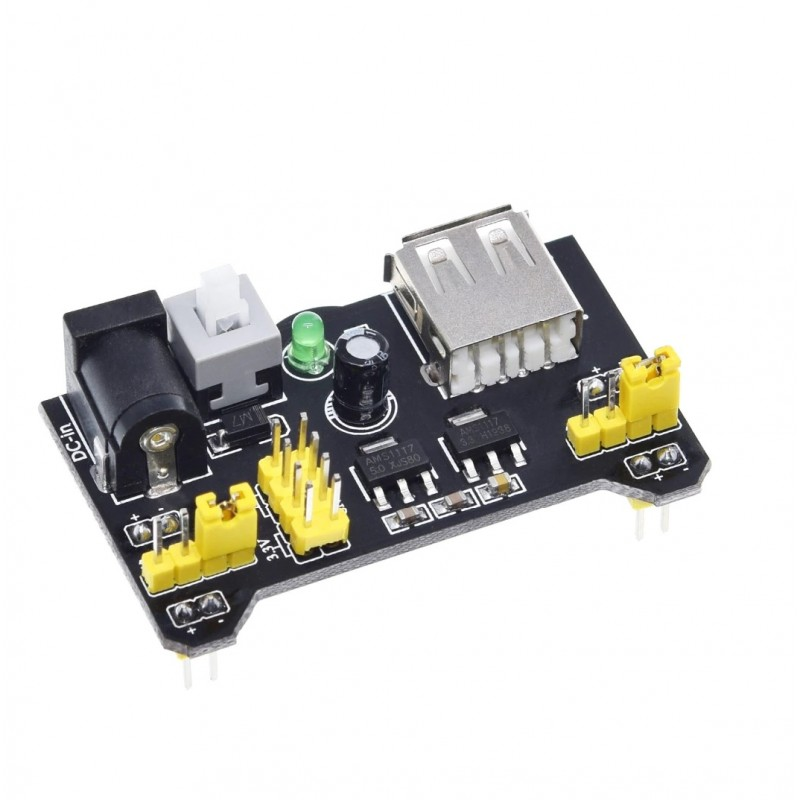
\includegraphics[width=0.25\linewidth]{Images/modulo-arduino-alimentacion.jpg}
         \caption{Mòdul alimentació 5V i 3,3V.}
         \label{modul_supply_fig}
     \end{figure}
     \item \textbf{Targeta microSD:} La targeta microSD on es guarden els arxius d'àudio en format .wav, és el model microSD Ultra de 8 GBytes.
    \begin{figure}[H]
        \centering
        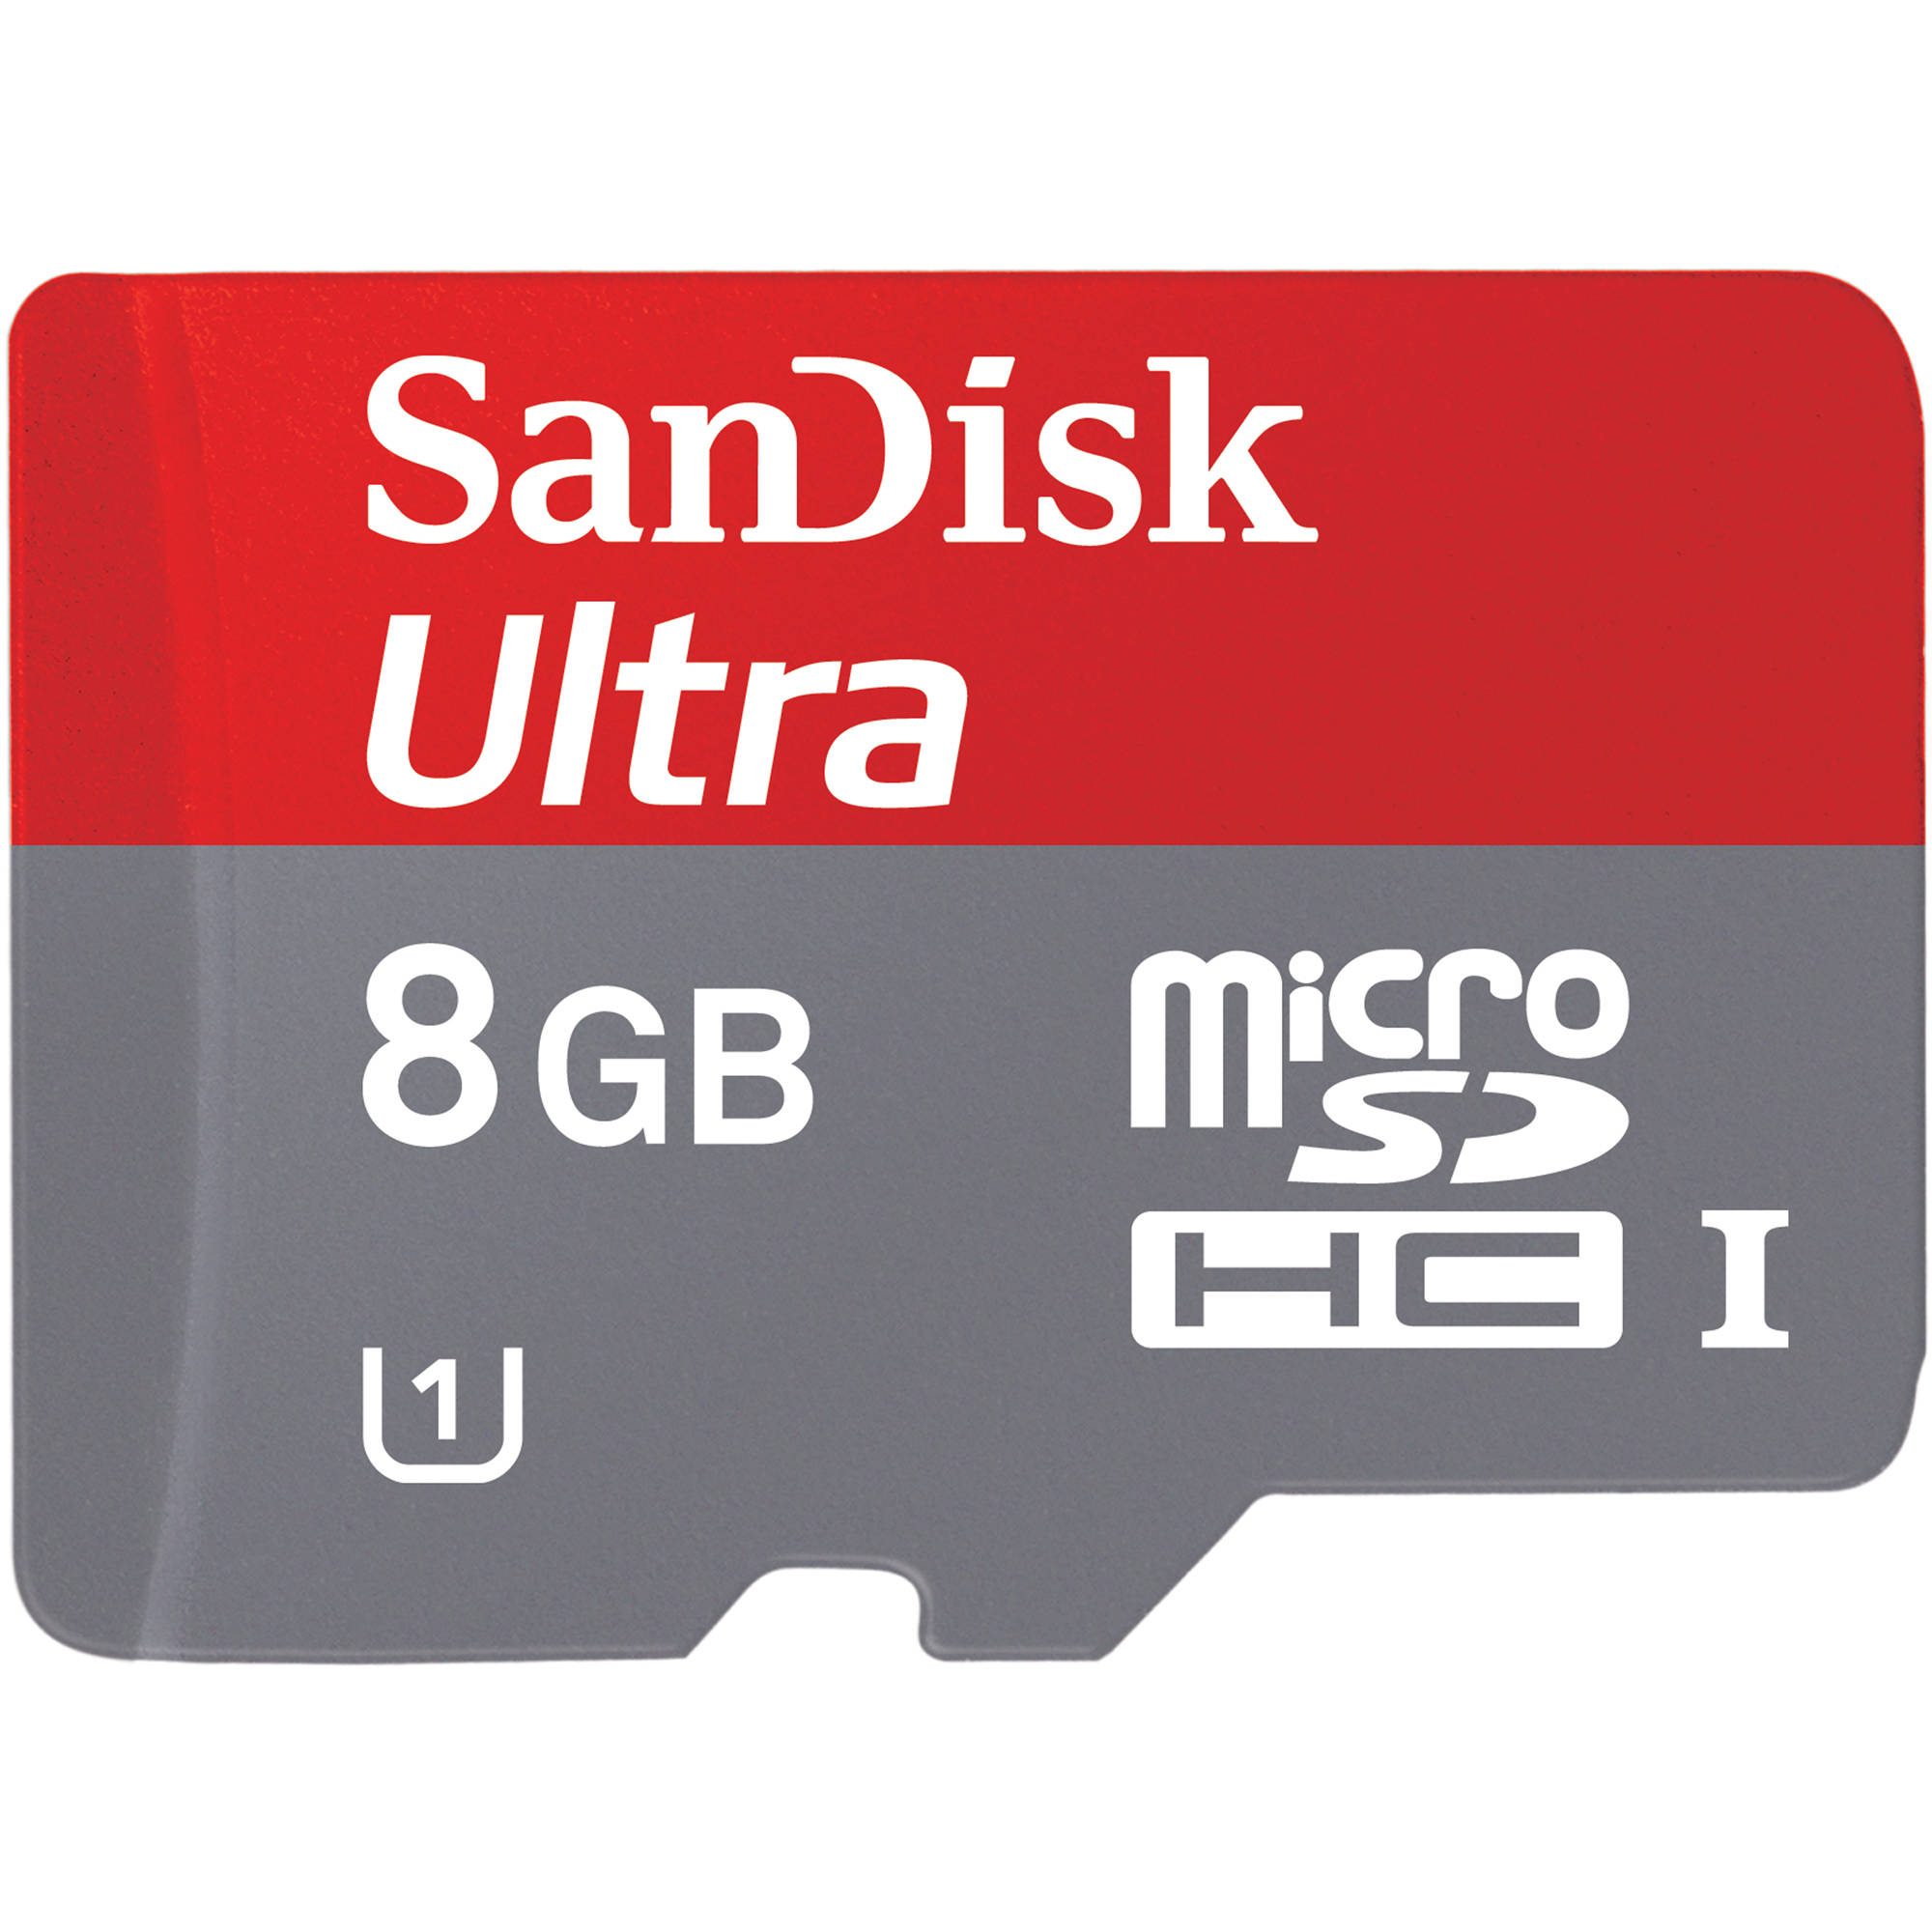
\includegraphics[width=0.15\linewidth]{Images/microsd_8gb.jpg}
        \caption{Targeta microSD amb 8 Gb de memòria.}
        \label{microSD_fig}
    \end{figure}
 \end{itemize}

\subsection{Llibreria SD.h}
\par La llibreria SD.h permet fer lectures de targetes SD i escriure-hi, tot utilitzant un seguit de funcions que a continuació es mencionen.
\par Per inicialitzar la targeta SD, cal cridar la funció \textit{begin()} i, si escau, especificar el pin de CS. La funció \textit{begin()} retorna una variable de tipus bool per poder determinar si s'ha inicialitzat correctament la comunicació amb la targeta SD.
\begin{figure}[H]
    \centering
    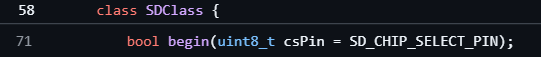
\includegraphics[width=0.5\linewidth]{Images/SD-begin_method.png}
    \caption{Mètode begin() de la classe SDclass. (font arduino o repo github)}
    \label{SD_begin_method_fig}
\end{figure}
\par Un cop inicialitzada correctament la targeta SD i el protocol SPI per la comunicació entre SD i ESP32, es poden obrir els fitxers emmagatzemats dins la SD. Amb la funció \textit{open(filepath)}, s'obre l'arxiu especificat al directori i en genera un objecte de la classe file o, en cas de no existir cap fitxer sota l'adreça de l'argument, retorna un false en booleà. D'aquesta forma, l'objecte generat a partir del fitxer permet fer ús dels mètodes de la classe file com llegir el seu contingut (\textit{read(*direcció memòria, longitud en bytes)}) i accedir a una direcció concreta dins la memòria (\textit{seek(*direcció memòria)}), entre d'altres.\cite{SDarduino}

\subsection{Llibreria I2S.h}
\par La targeta ESP32-WROOM-32 conté dos perifèrics I2S que es poden configurar per transmetre la informació en mode master o slave i actuar com un transmissor o receptor d'informació.
\par La targeta ESP32 s'ha configurat en mode master transmissora degut a les necessitats del sistema implementat.
\par Per configurar el mode de treball del canal I2S entre altres propietats, cal declarar l'struct \textit{i2s{\_}config{\_}t}. A la figura \ref{i2s_config_fig}, es pot observar la declaració de la variable constant de tipus estàtic \textit{i2s{\_}config} per configurar els paràmetres del protocol I2S. El primer atribut és el mode d'operació del port declarat, que és una variable de tipus enum. El mode predeterminat és de master transmissor \cite{I2SESP32code}. El segon atribut és la freqüència de sampleig de la informació transmesa pel bus. El tercer atribut és una nova variable enum, \textit{i2s{\_}bits{\_}per{\_}sample{\_}t}, que especifica el tamany de les mostres. L'atribut \textit{channel{\_}format} especifica el format de la trama del bus I2S. Com es comentarà més endavant, el format emprat és l'estàndard de Phillips, degut a que el transceiver dissenyat a la FPGA s'ha plantejat amb aquest mode d'operació. Per últim a destacar de l'struct \textit{i2s{\_}config}, l'atribut \textit{communication{\_}format} és una variable enum que especifica el format de comunicació de la mostra pel port SD. Els atributs que resten son per declarar la variable d'interrupció i els tamanys dels buffers emprats per la transmissió de les mostres, entre d'altres; es deixen en el mode predeterminat.

\begin{figure}[H]
    \centering
    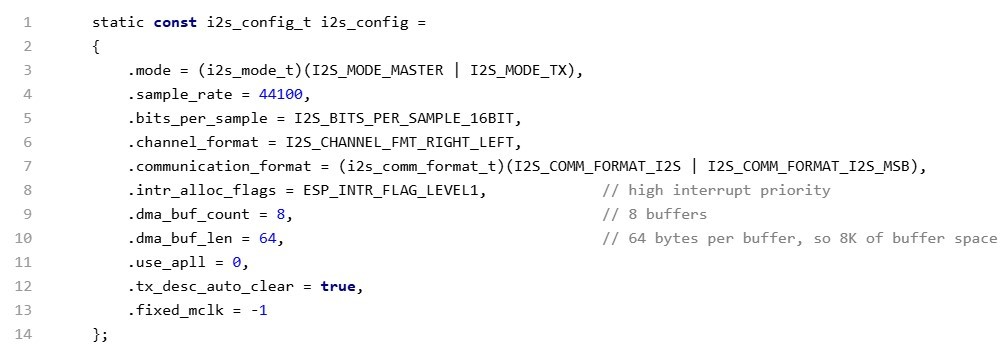
\includegraphics[width=0.7\linewidth]{Images/codi_i2sconfig.jpeg}
    \caption{Extracte del codi emprat per programar la targeta ESP32, on es declara la macro \textit{i2s\textunderscore config}.}
    \label{i2s_config_fig}
\end{figure}

\par Per configurar correctament el canal d'I2S caldrà assignar els pins del bus I2S als de la targeta ESP32. Per aquest motiu, es declara la variable estàtica \textit{pin{\_}config} com l'struct \textit{i2s{\_}pin{\_}config{\_}t}. Es pot observar a la figura \ref{pins_i2s_fig}, que els ports BCLK (o SCLK), WS i SD s'assignen a les macros declarades al principi de l'script. 
\begin{figure}[H]
    \centering
    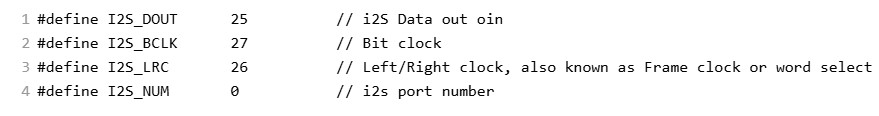
\includegraphics[width=0.7\linewidth]{Images/pins_i2s.jpeg}
    \caption{Declaració dels pins de la ESP32 assignats a cada senyal del bus I2S.}
    \label{pins_i2s_fig}
\end{figure}

\par Un cop declarades les variables de configuració esmentades, és necessari per inicialitzar el canal d'I2S correctament, fer ús de les següents funcions:
\begin{itemize}
    \item \textbf{\textit{i2s{\_}driver{\_}install}:} funció que instala el driver del protocol I2S a la ESP32 al port referenciat dins els arguments de la pròpia funció. A més, cal incluir en aquests arguments la variable \textit{i2s{\_}config} de configuració del canal.
    \item \textbf{\textit{i2s{\_}set{\_}pin}:} funció que assigna els pins del canal; utilitza la variable \textit{pin{\_}config} per configurar els ports amb els pins definits dins d'aquesta variable. 
\end{itemize}

\par Finalment, degut a que només es necessita enviar informació pel bus I2S, només serà necessari fer ús de la funció \textit{i2s{\_}write} que permet escriure la informació al buffer d'I2S. Entre els arguments de la funció està el port I2S de la targeta ESP32, la direcció dins la memòria on està emmagatzemada la informació a transmetre, el tamany en bytes de la mostra a enviar pel SD, una variable de control per saber els bytes que s'han enviat i per últim, els ticks d'espera del scheduler del RTOS implementat en la ESP32 per enviar la mostra pel buffer.\cite{I2SESP32code}

\subsection{Muntatge de la font d'àudio}
\par El muntatge final de la font d'àudio es pot observar a la figura \ref{fig_fontaudioI2S} amb els components mencionats en el primer apartat d'aquest capítol, interconnectats en una mateixa protoboard. El codi final amb el que s'ha programat la targeta ESP32 es pot trobar a l'Annex 1.
\begin{figure}[H]
    \centering
    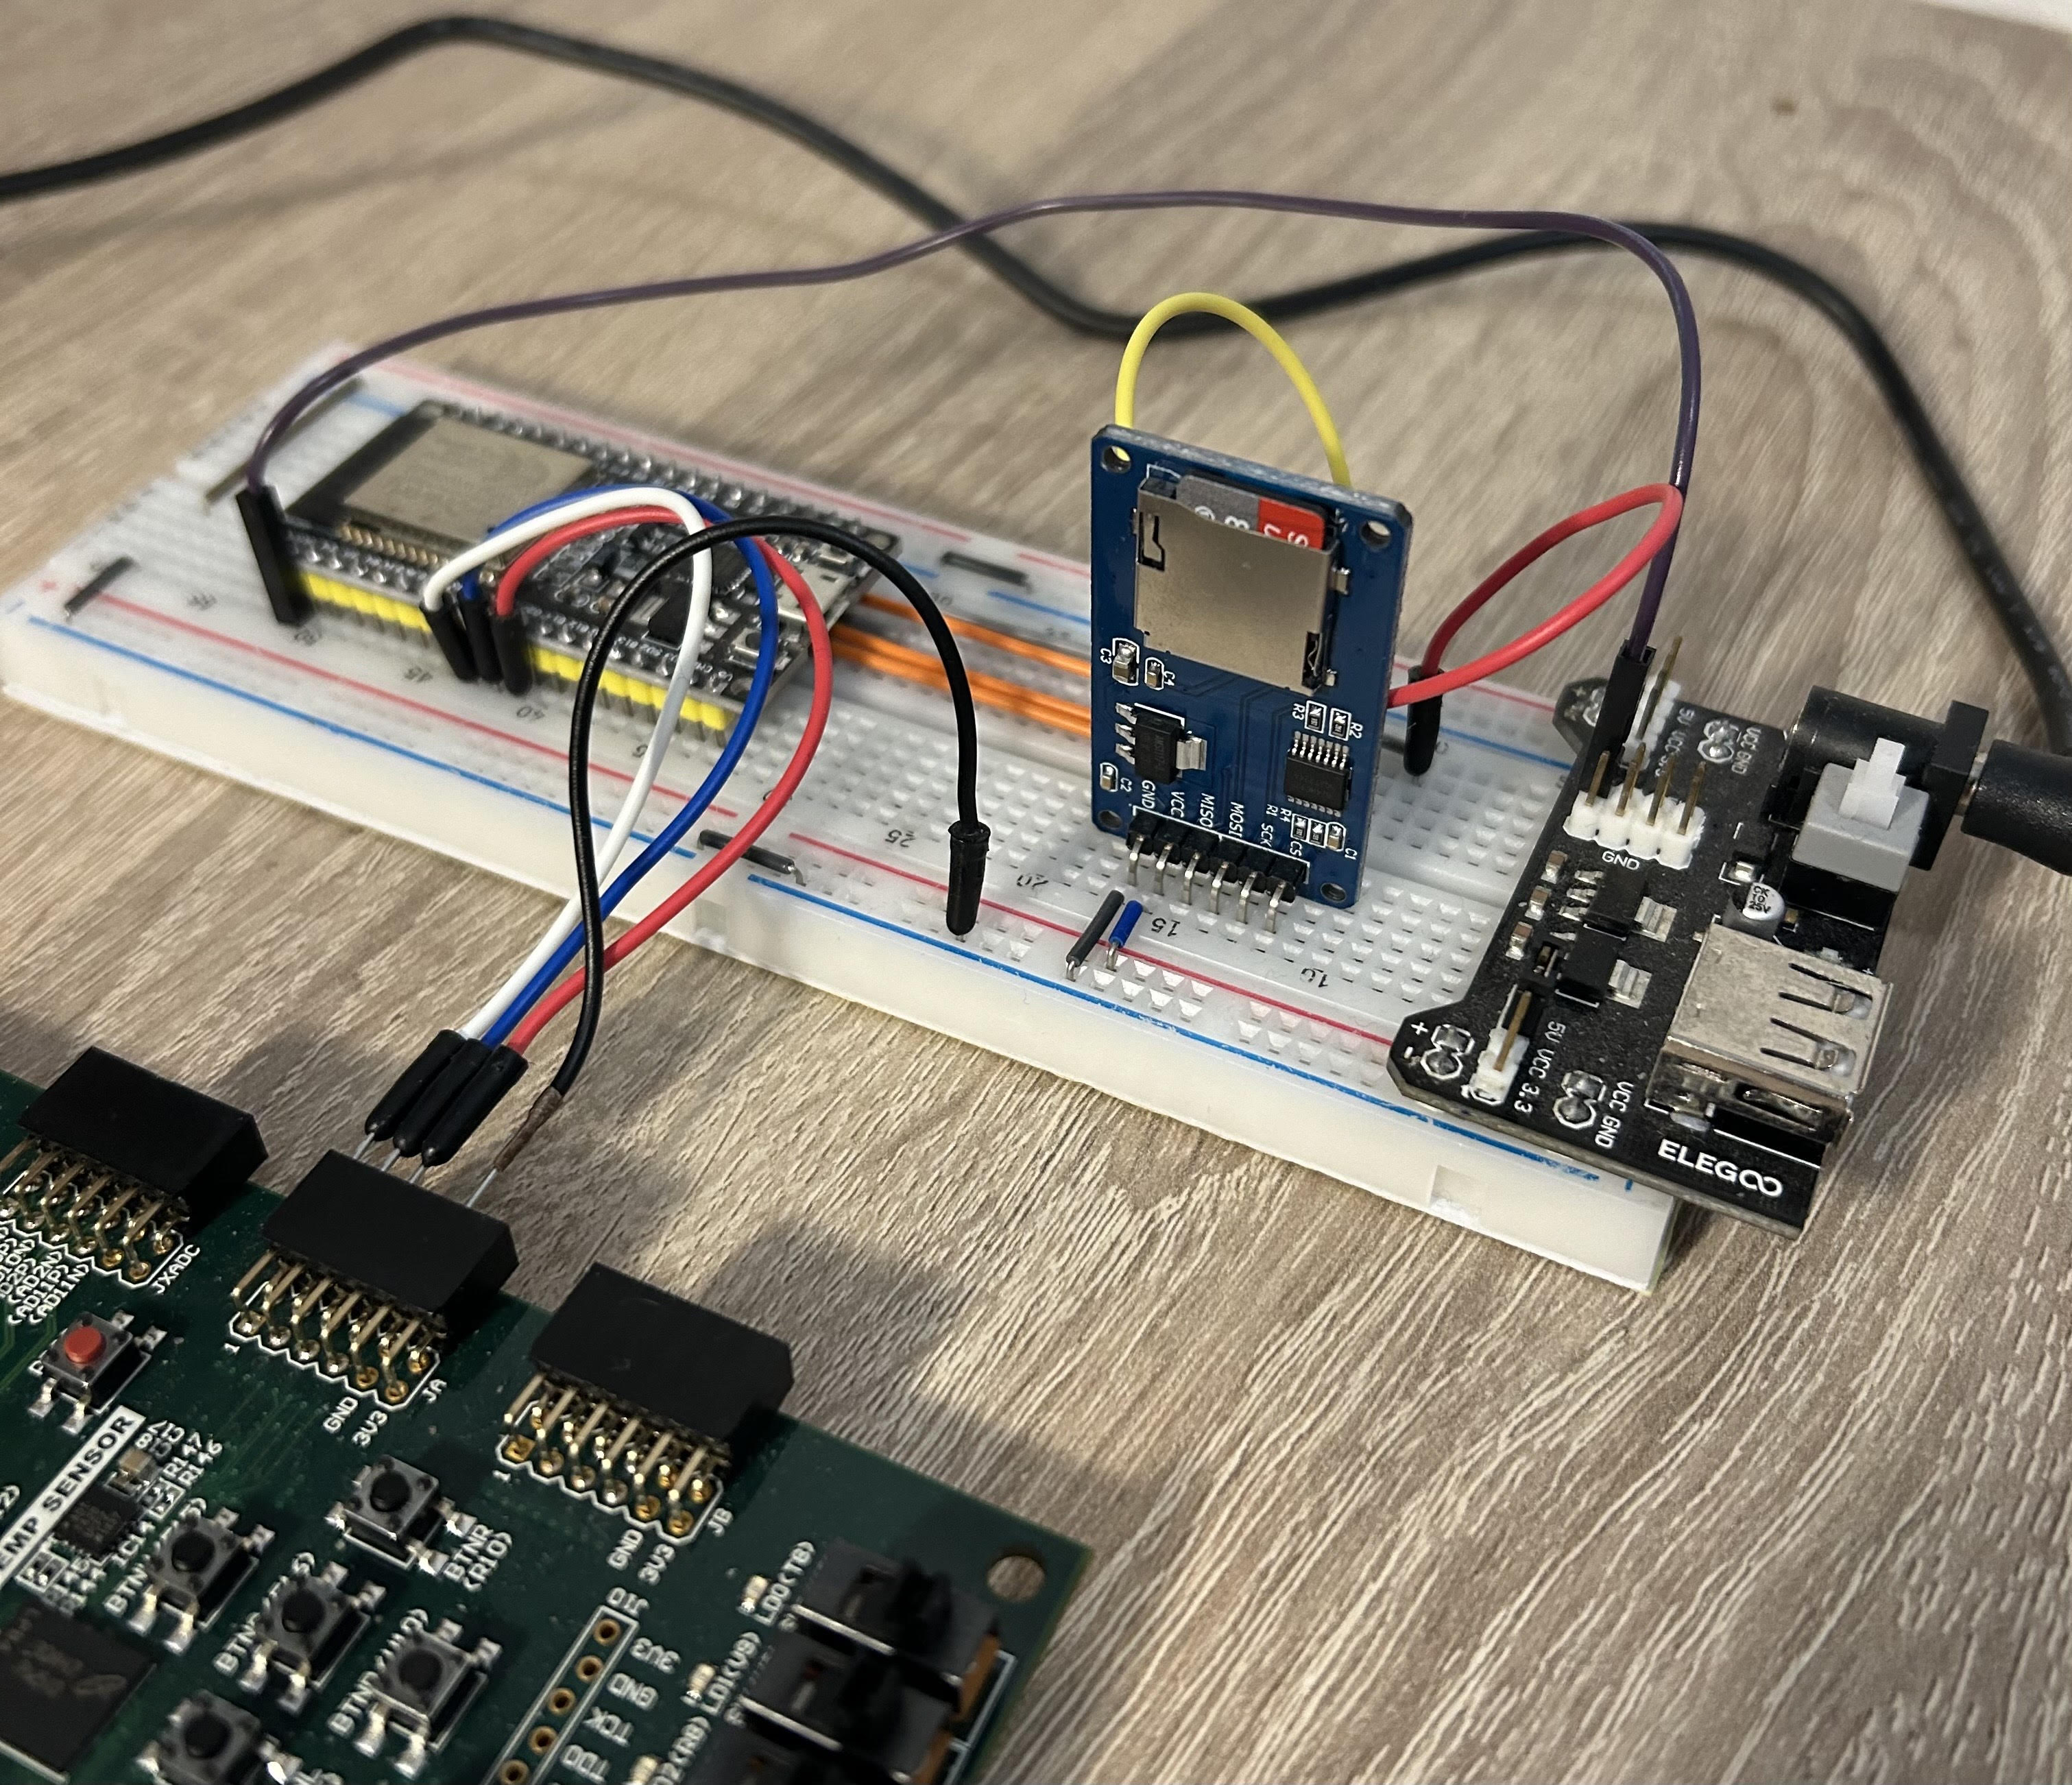
\includegraphics[width=0.4\linewidth]{Images/font_audio.jpg}
    \caption{Muntatge final de la font d'àudio I2S en una protoboard.}
    \label{fig_fontaudioI2S}
\end{figure}


 \section{Implementació del Receptor I2S}
 Per poder rebre correctament les mostres d'àudio transmeses pel bus I2S, s'ha dissenyat un receptor íntegrament en vhdl implementat a la FPGA. A continuació, es detalla el desenvolupament i execució del bloc.

 \subsection{Estructura de la entitat Receptora I2S}
 \par NXP (antigament Philips Semiconductors) ofereix possibles configuracions per la implementació del receptor I2S a \cite{I2S_manual}. A la figura \ref{receptor_i2s1_fig} es pot observar una d'aquestes configuracions. En aquest exemple, es pot apreciar que quan el senyal WS canvia de nivell, es genera un pols que provoca un reset del comptador de mòdul la longitud de la mostra d'àudio. Aquest comptador, genera polsos a les diferents senyals de sortida que activen els Flip Flops D i guarden el respectiu valor del bit. Quan WS canvia d'estat de nou, es transmet als registre de sortida del canal d'àudio que pertoqui, la mostra emmagatzemada en el conjunt de Flip Flops D i a continuació es resetejen. 

 \begin{figure}[H]
     \centering
     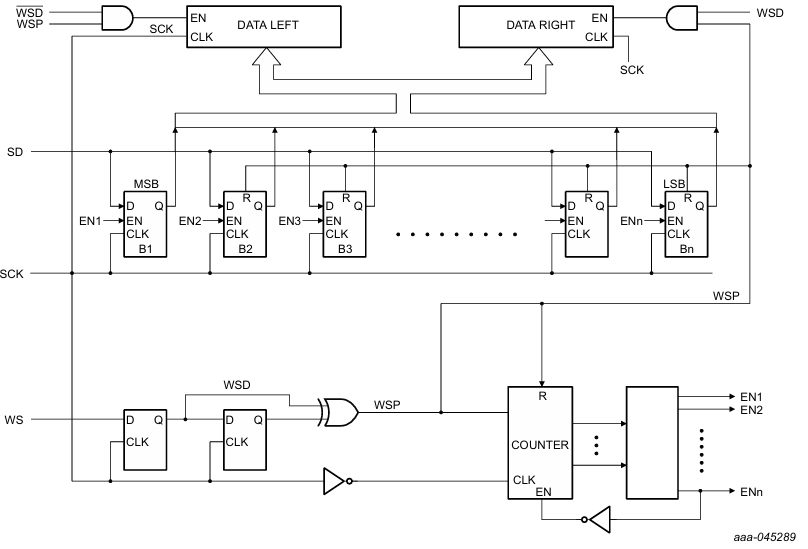
\includegraphics[width=0.6\linewidth]{Images/i2s_receiver_1.png}
     \caption{Una versió de la possible configuració del receptor I2S.\cite{I2S_manual}}
     \label{receptor_i2s1_fig}
 \end{figure}

 \par Una altra possible configuració que es mostren al manual \cite{I2S_manual} és la de la figura \ref{receptor_i2s2_fig}. En aquesta configuració, l'etapa de sortida és similar a la de la figura \ref{receptor_i2s1_fig}, essent composta de dos registres, un per canal d'àudio, i tants Flip Flops D com bits de la mostra samplejada. En aquesta implementació, el canvi d'estat del senyal WS també genera un pols que provoca un reset general dels Flip Flops de la sortida i del shift register que activa el Flip Flop D corresponent, segons el bit que s'està transmetent pel SD.
 \begin{figure}[H]
     \centering
     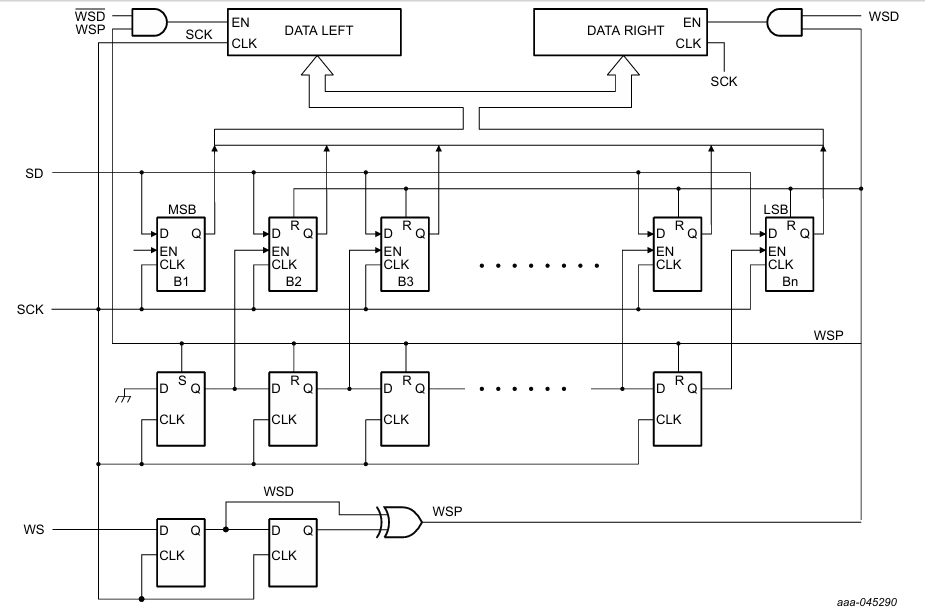
\includegraphics[width=0.6\linewidth]{Images/i2s_receiver_2.png}
     \caption{Una versió diferent de la figura \ref{receptor_i2s1_fig}, d'una possible configuració del receptor I2S. \cite{I2S_manual}}
     \label{receptor_i2s2_fig}
 \end{figure}

 \par Pel disseny del bloc receptor implementat a la FPGA s'han tingut en compte les configuracions comentades i finalment s'ha decidit per estructurar l'entitat com es pot veure a la figura \ref{diagrama_recI2S_fig}. El bloc receptor d'aquest treball implementa el comptador de bits de \ref{receptor_i2s1_fig} activat pel pols generat al canvi de nivell a WS. A diferència de les estructures exposades, la sortida es guarda en un registre SIPO. Un cop fet la lectura de la mostra transmesa pel bus I2S, es grava el valor en un registre PIPO.
 \begin{figure}[H]
     \centering
     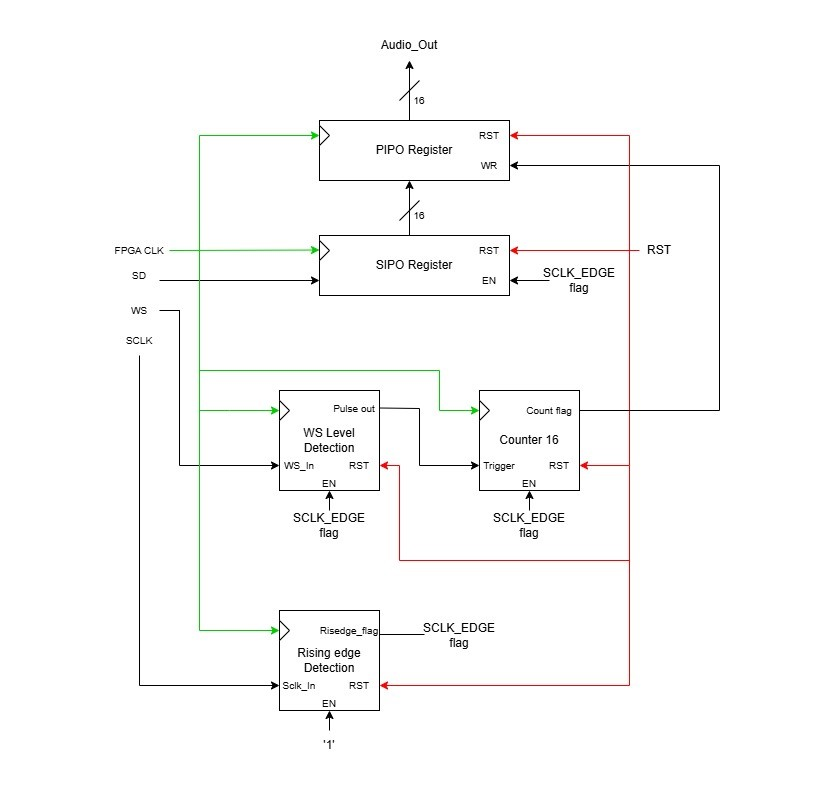
\includegraphics[width=0.55\linewidth]{Images/DiagramaTransceiverI2S.jpg}
     \caption{Diagrama de blocs de l'estructura implementada en el receptor I2S.}
     \label{diagrama_recI2S_fig}
 \end{figure}
 
 Els sub-blocs que el composen són els següents:
 \begin{itemize}
     \item \textbf{Rising Edge Detection:} Aquest bloc es un detector de flancs de pujada, que quan es detecta un canvi d'estat, de Low a High, es genera un pols al senyal de sortida. S'aplica a l'entrada el senyal SCLK per poder sincronitzar tots els blocs amb la flag de la sortida.
     \item \textbf{WS Level Detection:} El bloc genera un pols a la sortida quan el senyal d'entrada WS canvia d'estat. 
     \item \textbf{Counter 16:} Comptador de mòdul 16 que compta els flancs de pujada del SCLK. Quan arriba a 16, al port Count flag es genera un pols d'amplada un període del clk de la fpga, que activa la escriptura al registre PIPO de la sortida.
     \item \textbf{SIPO Register:} Registre SIPO per emmagatzemar el valor de la mostra d'àudio transmesa pel SD.
     \item \textbf{PIPO Register:} Registre PIPO on s'emmagatzema la mostra d'àudio a la sortida.
 \end{itemize}
 
\subsection{Banc de proves del receptor I2S}
\par Finalment, es procedeix a la validació de les funcionalitats del bloc receptor en conjunt. Degut a que l'entitat és de creació pròpia, és necessari testejar-lo amb un banc de proves. Per això, es simulen els senyals del bus I2S i el clock de la FPGA, tot mantenint els timings esperats. \par Com es pot apreciar a la figura \ref{figtestbenchI2S}, la mostra \textit{input\textunderscore 1} es captura a la sortida un cop s'han transmés els 16 bits de longitud del senyal. A continuació s'esmenen els requisits per al banc de proves:
\begin{itemize}
    \item \textbf{clock del sistema:} El període del clock del sistema és de 10 ns (100 MHz).
    \item \textbf{SCLK:} El període del serial clock del bus I2S esperat són 350 ns (2,85 MHz).
    \item \textbf{WS:} El període del WS esperat és de 32 cicles del rellotge sclk. 
    \item \textbf{SD:} Com ja s'ha explicat anteriorment, el mode d'operació del bus I2S és l'estàndard Philips, i en aquest mode, el MSB s'envia un període del sclk després del canvi al WS.
\end{itemize}
\begin{figure}[H]
    \centering
    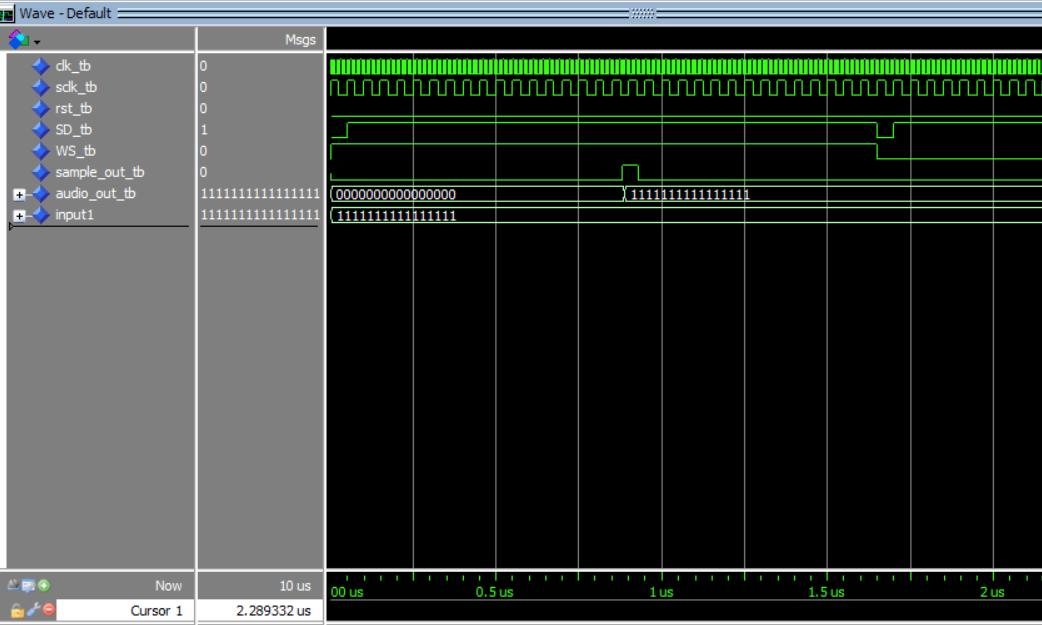
\includegraphics[width=0.6\linewidth]{Images/testbenchI2S.png}
    \caption{Cronograma del banc de proves pel receptor I2S.}
    \label{figtestbenchI2S}
\end{figure}

\section{Implementació a la FPGA}
\par Finalment, es sintetitza el codi VHDL del receptor al programa Vivado per evaluar els recursos consumits de la FPGA en la implementació del bloc. S'exposen els recursos de la FPGA utilitzats en la implementació del bloc a la taula \ref{taularecursosI2S}. Com es pot observar, el receptor I2S només utilitza blocs combinacionals per implementar les portes lògiques dels sub-blocs. En canvi, el major consum de recursos es deu als registres o blocs síncrons (FFs), que arriben a un total de 48.

\begin{table}[H]
    \centering
    \begin{tabular}{ | c | c | c | c | c | c |}
    \hline
    \centering
    \textbf{ID}     &  \textbf{LUTs} & \textbf{Registres}  & \textbf{Slices} & \textbf{Muxes}  & \textbf{DSPs} \\ [2ex] \hline
    \centering
    Receptor I2S    &  12 & 48  & 10 & 0  & 0 \\ \hline
    \end{tabular}
    \caption{Utilització de recursos de la FPGA pel bloc IP dissenyat.}
    \label{taularecursosI2S}
\end{table}

  
\chapter{Filtre d'Interpolació i Sobremostreig}
\section{Disseny del Filtre de l'Etapa d'Interpolació}
\par Per poder fer el modelat de soroll més endavant i obtenir el rendiment esperat, s'ha implementat una etapa de filtrat i interpolació que aplica un sobremostreig de OSR = 32 dividit en dues etapes. La primera etapa de filtrat es porta a terme en el bloc del filtre FIR, on es sobremostreja l'entrada d'àudio per un OSR = 2. Tot seguit, a l'etapa d'interpolació i filtrat del bloc CIC s'interpola el senyal amb un OSR = 16. En conjunt, els blocs formen el filtre anti-aliasing pre-modulació $\Sigma\Delta$, que millora el rendiment del procés, distribuint el soroll de quantificació inherentment acoblat al senyal d'àudio quantificat i atenua l'amplitud dels harmònics fora de l'ample de banda.    
\par Com s'ha comentat breument a l'apartat 4.6, els filtres CIC són una estructura molt popular en processadors DSP que implementen etapes de sobremostreig o delmat eficients en l'ús de recursos del Hardware. No obstant, per aconseguir una resposta en freqüència amb banda de pas plana i una banda de transició aguda, cal que el bloc CIC vagi precedit d'un filtre compensador. La resposta en freqüència dels filtres CIC ve donada per:
\begin{equation}\label{CIC_magintude_eq}
    \left| H_{CIC}(f) \right| = \left|\frac{1}{RM}\frac{sin(\pi Mf)}{sin(\frac{\pi f}{R})}\right|^N
\end{equation}
On M és el delay diferencial dels blocs Comb, R el factor d'interpolació i N l'ordre del filtre.
\par Com estratègia per aconseguir una banda de pas uniforme i de magnitud 0 dB, es pren la inversa de la magnitud del filtre CIC (equació \ref{CIC_magintude_eq}) per definir la funció de transferència del filtre de compensació. En aplicacions on el producte de R·M $\geq$ 10 i l'ordre del filtre CIC és $\leq$ 7, es pot assumir que la funció de transferència del filtre de compensació es simplifica per la inversa de la funció sinc.\cite{AN455}\cite{Hogenauer1981}
\begin{equation}\label{CIC_compensation_filter_eq}
    \left| H_{Compensation,CIC}(f) \right| = \left|RM\frac{sin(\frac{\pi f}{R})}{sin(\pi Mf)}\right|^N \approx \left| \frac{\pi Mf}{sin(\pi Mf)} \right| ^N = \left|sinc^{-1}(Mf) \right|^N
\end{equation}
\par Per poder calcular els coeficients del filtre de compensació i dimensionar correctament la resposta en freqüència de l'etapa de filtrat en conjunt, s'ha utilitzat el programa MATLAB\textsuperscript{\tiny\textregistered} per la àmplia llibreria disponible per aplicacions en el processament digital de senyals. 
\subsubsection{Filtre de Compensació}
\par Abans de trobar els coeficients que defineixin la resposta en freqüència del filtre, és necessari definir els requisits en rendiment que ha de complir i el context en que s'implementa. A continuació es declaren les especificacions del filtre a implementar:
\begin{table}[H]
    \centering
    \begin{tabular}{ | c | c | }
    \hline
    \centering
     Factor d'interpolació        &  2\\ \hline
     \centering
     Freqüència de pas            &  20 kHz\\ \hline
     \centering
     Freqüència de tall           &  22,05 kHz \\ \hline
     \centering
     Atenuació a la banda de tall &   80 dB\\ \hline
     \centering
     Freqüència de mostreig       &  44,1 kHz \\ \hline
    \end{tabular}
    \caption{Especificacions del filtre de compensació de l'etapa d'Interpolació.}
    \label{taula_filtre_compCIC}
\end{table}
\par Amb les especificacions de la taula \ref{taula_filtre_compCIC} es defineixen els atributs de l'objecte dsp.CICCompensationInterpolator i fent ús de la funció coeffs(), es retorna un vector dels coeficients del sistema. La funció coeffs() retorna un vector de longitud 153 valors que es correspon amb l'ordre del filtre FIR. A la figura \ref{Bode_CompCIC} es pot apreciar el diagrama de Bode del filtre dissenyat.
\begin{figure}[H]
    \centering
    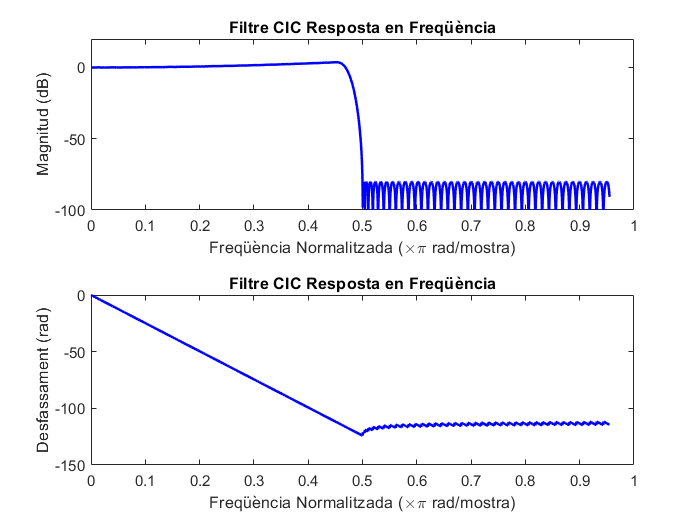
\includegraphics[width=0.5\linewidth]{Images/CIC_CompensationFilter.png}
    \caption{Diagrama de Bode del filtre de compensació de l'etapa d'Interpolació.}
    \label{Bode_CompCIC}
\end{figure}
\subsubsection{Filtre CIC}
A diferència del filtre de compensació, el filtre d'Interpolació CIC no requereix càlculs dels coeficients, degut a que no en té. La resposta en freqüència del filtre en qüestió ve donada per tres paràmetres enters (R, M i N) i la freqüència de mostreig del senyal d'entrada. Modificant el delay diferencial M es pot controlar l'ubicació dels zeros del sistema i en conseqüència la resposta en freqüència. Aquests zeros apareixen en múltiples de $\frac{1}{M}$ i a les regions del voltant d'aquests nuls es produeix l'efecte de l'aliasing. Específicament, aquestes bandes d'àlies són \[(i-f_c) \leq f < (i + f_c)\] per a f $\leq$ $\frac{1}{2}$ i i= 1,2...,[R/2]. Típicament, el paràmetre M sol prendre els valors 1 o 2 permetent una optimització de la implementació del filtre CIC. 
\par Per poder aconseguir la màxima atenuació del soroll en la banda de rebuig o d'aturada, cal modelar l'ordre del filtre fins arribar al valor d'atenuació desitjat. Degut a que la freqüència de Nyquist del senyal passarà a situar-se a R·$f_{Nyquist}$, interessa atenuar el màxim possible la banda de rebuig del senyal original. 
\par Finalment, s'ha trovat que els valors R, M i N del filtre CIC que millor s'adapten als requisits globals de l'etapa de filtrat i sobremostreig són els següents:
\begin{table}[H]
    \centering
    \begin{tabular}{ | c | c | }
    \hline
    \centering
     Factor d'interpolació (R)       &  16\\ \hline
     \centering
     Delay diferencial (M)       &  1\\ \hline
     \centering
     Ordre del filtre CIC (N)        &  5 \\ \hline
    \end{tabular}
    \caption{Especificacions del filtre CIC.}
    \label{taula_filtre_CIC}
\end{table}
\begin{figure}[H]
    \centering
    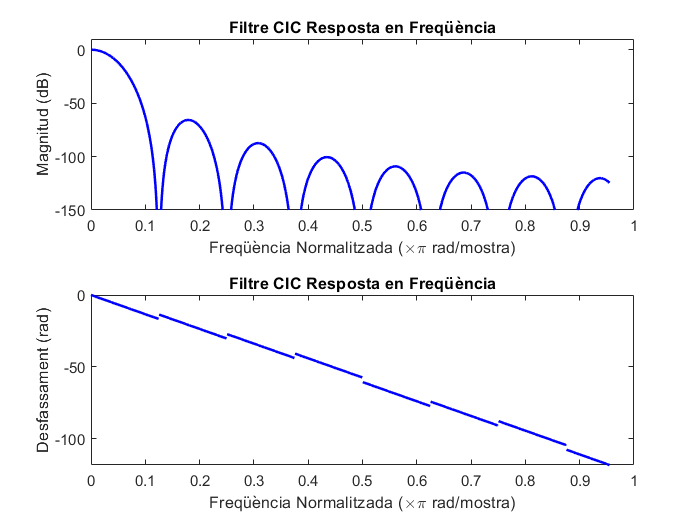
\includegraphics[width=0.5\linewidth]{Images/CIC_Filter.png}
    \caption{Diagrama de Bode del filtre CIC}
    \label{CIC_Bode_fig}
\end{figure}

\subsubsection{Etapa de filtrat i sobremostreig en sèrie}
\par Finalment, situant les dues etapes en sèrie es troba la resposta en freqüència del filtre anti-aliasing. En la figura \ref{fig_BodeEtapaFiltre}, es pot apreciar com la resposta en magnitud a la banda de pas és plana fins la freqüència de tall a $f_c$ = 0,029 $\pi$ rad/mostra, que equival a 20,4 kHz, aproximadament la freqüència de tall de disseny del filtre de compensació (taula \ref{taula_filtre_compCIC}). També es pot apreciar com les imatges ubicades en les proximitats dels zeros del filtre CIC, es veuen atenuades per 50 dB. La resposta en fase decreix linealment, fet que suggereix que el sistema és aproximadament lineal en fase en la banda de pas. La linealitat en la resposta en fase a la banda de pas és rellevant per l'aplicació d'aquest treball degut que en els senyals d'àudio la distorsió de fase provoca anomalies acústiques perceptibles per l'oïda humana. A la taula \ref{taula_mesuresEtapaInterp} estan plasmades les especificacions del etapa d'interpolació del filtre dissenyat.
\begin{figure}[H]
    \centering
    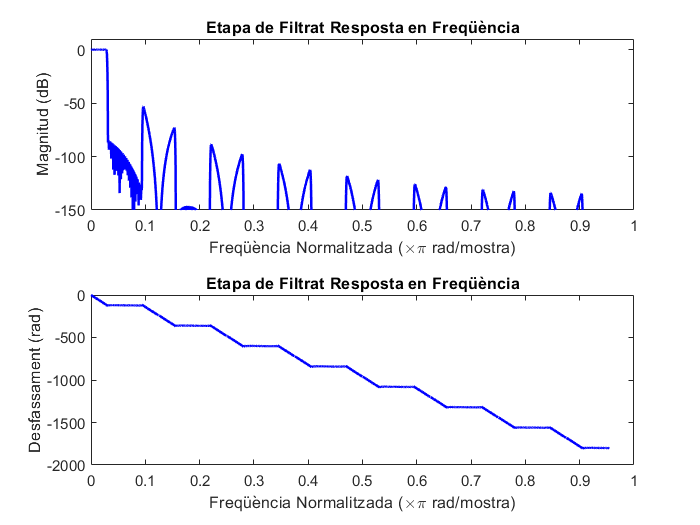
\includegraphics[width=0.5\linewidth]{Images/Etapa_FiltreInterp.png}
    \caption{Diagrama de Bode de l'etapa de filtrat i sobremostreig dissenyada.}
    \label{fig_BodeEtapaFiltre}
\end{figure}
\begin{table}[H]
    \begin{center}
    \begin{tabular}{ | c | c | }
        \hline
        \centering
        Oscil·lació màxima en la banda de pas & 1.49 dB \\ \hline
        \centering
        Freqüència de tall   &  20460 Hz\\ \hline
        \centering
        Atenuació en la banda de tall & -53 dB \\ \hline
    \end{tabular}
    \end{center}
    \caption{Especificacions de l'etapa de filtrat i sobre-mostreig.}
    \label{taula_mesuresEtapaInterp}
\end{table}


\section{Mòdul IP FIR Compiler}
\par Per a la implementació de la primera etapa del filtratge a la FPGA, s'ha utilitzat el mòdul LogiCORE IP FIR Compiler \cite{FIRcompiler}. Aquest bloc permet la sintetització del filtre dissenyat, optimitzant l'utilització dels recursos disponibles a la pròpia FPGA. Per poder implementar el filtre dissenyat en el mòdul en qüestió, cal configurar els paràmetres d'implementació correctament. 
\begin{table}[H]
    \centering
    \begin{tabular}{ | c | c | }
    \hline
    \centering
    \textbf{Nom del Paràmetre}     &  \textbf{Valor}\\ [2ex] \hline
    \centering
    Tipus de Filtre    &    Interpolació \\ \hline
    \centering
    Taxa d'interpolació    &    2 \\ \hline
    \centering
    Format d'Oversampling pel Hardware &    Especificació per freqüència \\ \hline
    \centering
    Freqüència de mostreig d'entrada & 0,0441 MHz \\ \hline
    \centering
    Freqüència de rellotge &    100 MHz \\ \hline
    \centering
    Tipus de coeficients &  Amb signe \\ \hline
    \centering
    Amplada Coeficients & 153 \\ \hline
    \centering
    Tipus de dades d'entrada &  Amb signe \\ \hline
    \centering
    Amplada dades d'entrada &   16 \\ \hline
    \centering
    Mode d'arrodoniment a la sortida & Truncar els LSB \\ \hline
    \centering
    Amplada dades de sortida &  16\\ \hline
    \end{tabular}
    \caption{Configuracions dels paràmetres del mòdul FIR Compiler.}
    \label{taula_configFIR}
\end{table}

\par Inclòs en el mòdul IP hi ha adjunt els arxius de simulació que permeten validar el funcionament del bloc i els respectius pins. A \cite{FIRcompiler} defineixen els pins, destacant-ne els que poden ser d'utilitat per a l'aplicació de la etapa de preacondicionament per la posterior interpolació del filtre CIC:
\begin{itemize}
    \item \textit{aclk}: Entrada del rellotge a la que funcionen els blocs MAC.
    \item \textit{\texttt{s\_axis\_data\_tvalid}}: Entrada que determina en quin instant s’introdueix una mostra.
    \item \textit{\texttt{s\_axis\_data\_tready}}: Sortida que indica que l’estat del filtre és correcte. Cal que aquesta sortida estigui a 1 sempre que el filtre estigui actiu. 
    \item \textit{\texttt{s\_axis\_data\_tdata}}[15:0]: Entrada del vector del valor mostrejat.
    \item \textit{\texttt{m\_axis\_data\_tdata}}[23:0]:  Vector de sortida de la mostra filtrada.
\end{itemize}
\begin{figure}[H]
    \centering
    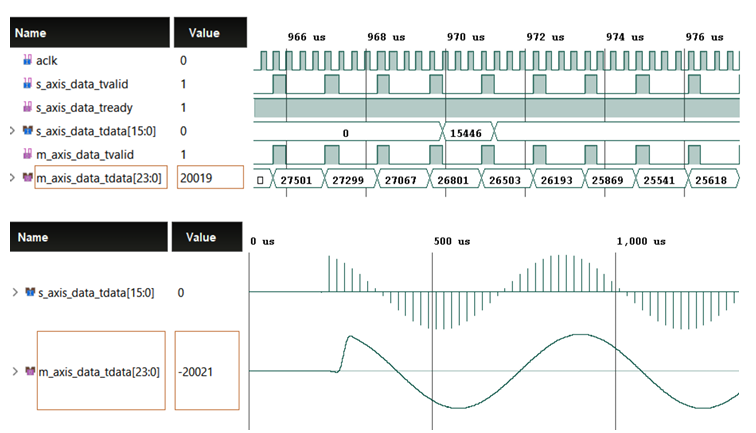
\includegraphics[width=0.6\linewidth]{Images/FIRcompilerTestbench.png}
    \caption{Cronograma del testbench del bloc IP FIR Compiler \cite{TFGAmpClassD}}
    \label{figFIRtestbench}
\end{figure}


\section{Mòdul IP CIC Compiler}
\par Per últim, l'etapa d'Interpolació del CIC s'executa amb el mòdul LogiCORE IP CIC Compiler. Similar al mòdul IP del filtre FIR, aquest permet configurar també els seus paràmetres d'implementació que venen especificats en la taula següent:
\begin{table}[H]
    \centering
    \begin{tabular}{ | c | c | }
    \hline
    \centering
    \textbf{Nom del Paràmetre}     &  \textbf{Valor}\\ [2ex] \hline
    \centering
    Tipus de Filtre    &    Interpolació \\ \hline
    \centering
    Nombre d'etapes    &    5 \\ \hline
    \centering
    Format d'Oversampling pel Hardware &    Especificació per freqüència \\ \hline
    \centering
    Freqüència de mostreig d'entrada & 0,0882 MHz \\ \hline
    \centering
    Freqüència de rellotge &    100 MHz \\ \hline
    \centering
    Amplada dades d'entrada &   16 \\ \hline
    \centering
    Quantització & Truncament \\ \hline
    \centering
    Amplada dades de sortida &  16\\ \hline
    \end{tabular}
    \caption{Configuracions dels paràmetres del mòdul CIC Compiler.}
    \label{taula_configCIC}
\end{table}
\par El mòdul CIC Compiler comparteix el mateix pinatge que el bloc FIR Compiler degut a que ambdós blocs són compatibles amb el bus AXI4 intern de la FPGA. 
\par A la figura \ref{figCICtestbench} es pot apreciar com per cada mostra al pin d'entrada s\textunderscore data\textunderscore t\textunderscore data, es generen 16 mostres a la sortida del bloc.

\begin{figure}[H]
    \centering
    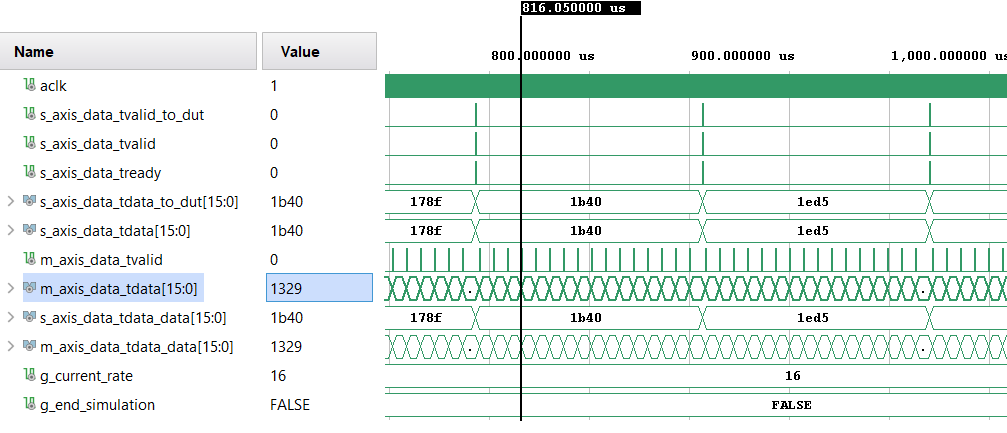
\includegraphics[width=0.6\linewidth]{Images/CICtestbench.png}
    \caption{Cronograma del testbench del bloc IP CIC Compiler.}
    \label{figCICtestbench}
\end{figure}

\section{Implementació a la FPGA}
\par Finalment, la implementació de l'etapa de filtrat i sobremostreig dissenyada en aquest capítol consumeix els recursos detallats a la taula \ref{taularecursosfiltre}. En aquesta taula, destaca l'àmplia utilització de LUTs per part del fir\textunderscore compiler i l'optimització en l'ús dels blocs DSP en els dos mòduls IP.

\begin{table}[H]
    \centering
    \begin{tabular}{ | c | c | c | c | c | c |}
    \hline
    \centering
    \textbf{ID}     &  \textbf{LUTs} & \textbf{Registres}  & \textbf{Slices} & \textbf{Muxes}  & \textbf{DSPs} \\ [2ex] \hline
    \centering
    fir\textunderscore compiler     &  454 & 268  & 79 & 46  & 1 \\ \hline
    \centering
    cic\textunderscore compiler     &  138 & 226  & 56 & 0  & 2 \\ \hline
    \end{tabular}
    \caption{Utilització de recursos de a la FPGA per cada bloc que conforma el filtre antialiasing.}
    \label{taularecursosfiltre}
\end{table}


\chapter{Modulació $\Sigma \Delta$}
\section{Disseny i evaluació de la topologia del modulador $\Sigma\Delta$}
\par En aquest treball, s'ha optat per implementar una etapa de modulació $\Sigma\Delta$ com estratègia per fer més efectiu el rebuig del soroll que incorporen les mostres d'àudio per diversos efectes, e.g. el procés de quantització. S'estudien els efectes d'implementar un modulador $\Sigma\Delta$ de segon ordre amb realimentació negativa,i com a referència per a la posterior comparació, es prenen els càlculs presentats a l'apartat 4.7 per un modulador $\Sigma\Delta$ de primer ordre. 
\par Un dels principals motius per fer l'estudi d'un modulador de segon ordre, és la implementació aparentment trivial a la FPGA degut a la manca de coeficients a diferència d'altres topologies (veure apartat 4.7). No obstant, la presència de dos llaços de realimentació i dos integradors en el modulador $\Sigma\Delta$ de segon ordre, comporta una possible deriva de l'estabilitat del sistema si no es prenen les consideracions adequades. A la figura \ref{fig_SigmaDelta} es pot visualitzar l'estructura que es pretén implementar, on els blocs H(z) representen els integradors i els valors $a_1$,$a_2$ els coeficients de pre-acondicionament.
\begin{figure}[H]
    \centering
    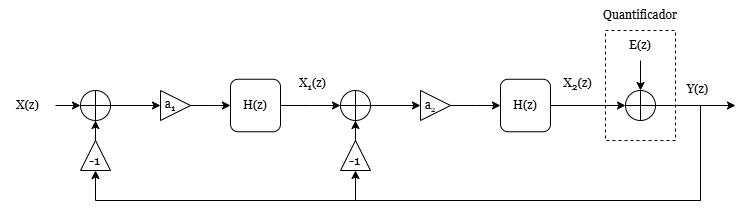
\includegraphics[width=0.7\linewidth]{Images/SigmaDelta.drawio.png}
    \caption{Diagrama de blocs d'un modulador $\Sigma\Delta$ de segon ordre.}
    \label{fig_SigmaDelta}
\end{figure}
\par De la figura \ref{fig_SigmaDelta}, cal destacar com el bloc Quantificador es pot modelar com la addició d'un senyal d'error E(z) assumint que el procés és lineal. Aquesta última aproximació de l'error de quantificació permet modelitzar el tractament del soroll i caracteritzar la resposta en freqüència. 
\par En el disseny d'aquest modulador $\Sigma \Delta$, el quantificador de la sortida és de 2 nivells amb una rebuig del soroll de quantificació esperat de 70 dB. Amb l'equació \ref{eq_SQNR}, es troba que per complir les especificacions s'ha de produir un sobremostreig de OSR = 32. Per tant, de \cite{UndrstndSDM} es defineix que la freqüència de mostreig a l'entrada del modulador amb $f_B$ = 20 kHz, ha de ser de:
\begin{equation}
    f_{s_{min}} = 2\ OSR\ f_B = 1,28\ MHz
\end{equation}
\par La seqüència de sortida està representada per Y(z) i la sortida de cada integrador ve donada per la seva variable d'estat, $X_1$(z) i $X_2$(z) per al primer i el segon integrador, respectivament. El sistema d'equacions es pot escriure de la següent forma:
\begin{equation}\label{eq_sistemaSDM}
    \left\lbrace\begin{array}{c}  X_1(z) = a_1 H(z) (X(z)-Y(z)) \\ X_2(z) = a_2 H(z) (X_1(z)-Y(z)) \\
    Y(z) = X_2(z) + E(z)\end{array}\right.
\end{equation}
Resolguent el sistema \ref{eq_sistemaSDM}, es troba que la funció de transferència del Senyal (STF) i del Soroll (NTF) s'expressen de la següent forma:
\begin{equation}\label{eq_STF}
    STF(z) = \frac{a_1 a_2 H^{2}(z)}{a_1 a_2 H^{2}(z) + a_2 H(z) + 1}
\end{equation}
\begin{equation}\label{eq_NTF}
    NTF(z) = \frac{1}{a_1 a_2 H^{2}(z) + a_2 H(z) + 1}
\end{equation}
\par Per poder trobar el valor dels coeficients de pre-acondicionament, cal estudiar l'estabilitat del sistema en temps continu. Per tant, s'analitza el sistema amb la variable de Laplace (s) i es considera la funció de transferència del bloc integrador com:
\begin{equation}\label{eq_intLaplace}
  H(s) = \frac{1}{T_s s}  
\end{equation} 
\par Les equacions \ref{eq_STF} i \ref{eq_NTF} es poden transformar a la variable de Laplace simplement substituint el bloc integrador per l'equació \ref{eq_intLaplace}. Per evaluar l'estabilitat del sistema, es troba que el denominador de la funció de transferència s'expressa de la següent forma:
\begin{equation}\label{eq_dentransf}
    D(s) = s^2 + \frac{a_2}{T_s} s + \frac{a_1 a_2}{T_s}
\end{equation}
\par Aplicant el criteri de Routh-Hurwitz, el sistema és estable per $a_1$, $a_2$ $>$ 0. Com a \cite{ADC16b}, s'assigna als coeficients de pre-acondicionament $a_1$=$a_2$=0,5 degut a que en operacions binàries el producte per $\frac{1}{2}$ equival a desplaçar el vector de bits 1 bit a l'esquerra.
\par Tornant de nou al temps discret, la funció de transferència dels blocs integradors en la variable z ve donada per:
\begin{equation}\label{eq_IntZ}
    H(z) = \frac{z^{-1}}{1 - z^{-1} }
\end{equation}
\par Amb els nous valors de $a_1$ i $a_2$, i la funció de transferència \ref{eq_IntZ}, les funcions de transferència \ref{eq_STF} i \ref{eq_NTF} resulten en: 
\begin{equation}\label{eq_STFsimpl}
    STF(z) = \frac{z^{-2}}{3z^{-2}-6z^{-1}+4}
\end{equation}
\begin{equation}\label{eq_NTFsimpl}
    NTF(z) = \frac{(1-z^{-1})^2}{3z^{-2}-6z^{-1}+4}
\end{equation}
\par Es pot observar a \ref{eq_STFsimpl} com el senyal d'entrada està retardada 2 mostres ($z^{-2}$), mentres l'error de quantificació està modelat pel terme (1-$z^{-1}$)$^2$ \cite{ADC16b}. Les expressions \ref{eq_STFsimpl} i \ref{eq_NTFsimpl} representen un filtre passa-baixos de les mostres samplejades i un filtre passa-alts per l'error de quantificació, respectivament. Aquest comportament caracteritza els moduladors $\Sigma \Delta$, ja que permet filtrar el senyal d'interès en la banda de pas, desplaçant l'error de quantificació cap a freqüències més altes. Això contribueix a una millora significativa de la relació senyal-soroll (SNR) del senyal portador d'àudio, fet que es tradueix en una qualitat sonora superior. 
\par Per analitzar l'estabilitat del sistema implementat i poder valorar la resposta en freqüència, es resolen les arrels del denominador de \ref{eq_STFsimpl} i \ref{eq_NTFsimpl}:
\begin{equation}\label{eq_polesSTF}
    0 = 4z^{2}-6z+3 \longrightarrow z_p = \frac{3}{4} \pm \frac{\sqrt{3}}{4}i
\end{equation}
\begin{equation}\label{eq_module_poleszSTF}
    \left|z_p\right| = \frac{\sqrt{3}}{2} = 0,866
\end{equation}
\begin{equation}\label{eq_angle_poleszSTF}
    \left|\theta_p\right| = 0,523\ rad
\end{equation}
\begin{figure}[H]
    \centering
    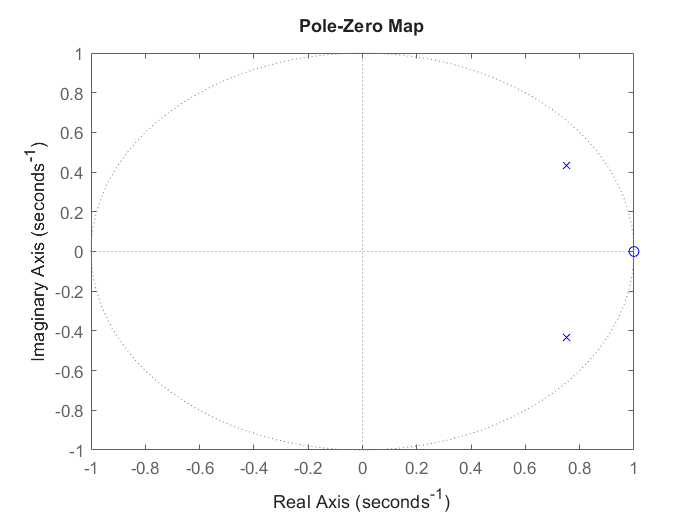
\includegraphics[width=0.5\linewidth]{Images/zeropoleMapMOD2.png}
    \caption{Cercle unitari en el pla polar de STF(z) i NTF(z). STF(z) i NTF(z) comparteixen pols.}
    \label{figzeropoleMap}
\end{figure}
\par Amb \ref{eq_module_poleszSTF} es pot verificar que els pols estan ubicats dins del cercle unitari, i per tant, es dedueix que el sistema es estable aparentment. Addicionalment, es possible trobar la freqüència que s'amplifica en la banda de pas tant de la funció de transferència del senyal d'entrada (STF) com en la del modelat del soroll (NTF), a partir de l'angle dels pols respecte l'eix real del pla polar (\ref{eq_angle_poleszSTF}). Només cal fer la transformació de freqüència en rad/mostra a Hz aplicant una simple regla de tres.
\begin{equation}\label{eq_cornerfreq}
    f_{peak} = \frac{\theta_{p}}{2\pi}\ f_{sample} = \frac{0,523}{2\pi}1,41\times 10^6 = 117,46\ kHz
\end{equation}
\begin{equation}\label{eq_magn_wnSTF}
    \left| STF(\theta_p)\right| = 6\ dB
\end{equation}
\begin{equation}\label{eq_magn_wnNTF}
    \left| NTF(\theta_p)\right| = 6,5\ dB
\end{equation}
\par Això ens permetrà dimensionar el sistema de forma més precisa per valorar posteriorment com es comporta el sistema en conjunt.
\par Per poder trobar la freqüència de tall del bloc es resol l'equació \ref{eq_STFsimpl} igualant-la a 0,707, que equival al decaïment de 3 dB en la banda de pas de la funció de transferència. S'aplica el mateix procediment a l'equació \ref{eq_NTFsimpl} per trobar a partir de quina freqüència deixa d'atenuar l'error de quantificació. 
\begin{equation}\label{eq_fcorteSTF}
    \left| STF(z)\right| = 0,707 \longrightarrow f_{c,STF} = 183,6\ kHz
\end{equation}
\begin{equation}\label{eq_fcorteNTF}
    \left| NTF(z)\right| = 0,707 \longrightarrow f_{c,NTF} = 77,95\ kHz
\end{equation}
\par Finalment, es procedeix a dimensionar el bloc $\Sigma \Delta$ de segon ordre dissenyat i s'exposen les característiques de rendiment a la taula \ref{taula_SigmaDelta}. 

\begin{table}[H]
    \centering
    \begin{tabular}{ | c | c | }
    \hline
    \centering
    SNQR     &  70.1 dB\\ \hline
    \centering
    DR    &    112,28 dB \\ \hline
    \centering
    OSR    &    32 \\ \hline
    \centering
    $fs_{in}$   &    1,41 MHz \\ \hline
    \centering
    $f_{tall, STF}$    &   183,6 kHz\\ \hline
    \centering
    $f_{tall, NTF}$    &   77,95 kHz\\ \hline
    \centering
    $f_{peak, STF}$    &   117,46 kHz\\ \hline
    \centering
    $f_{peak, NTF}$    &   117,46 kHz\\ \hline
    \end{tabular}
    \caption{Taula de les mètriques de rendiment calculades pel modulador $\Sigma \Delta$ dissenyat.}
    \label{taula_SigmaDelta}
\end{table}
\begin{figure}[H]
    \centering
    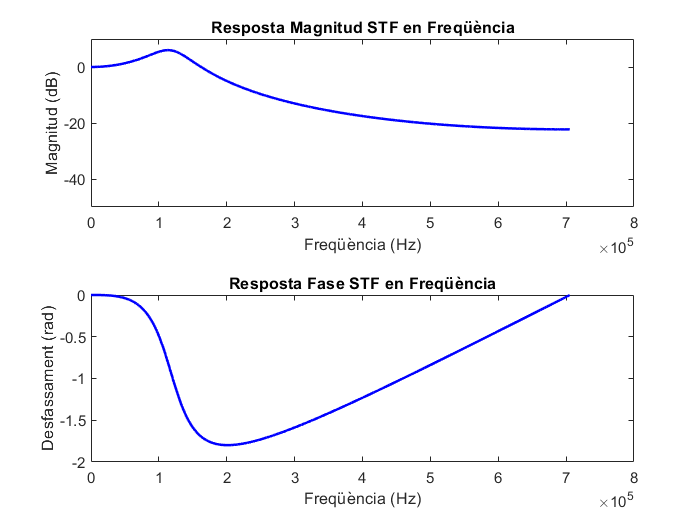
\includegraphics[width=0.5\linewidth]{Images/bodeSTFMOD2.png}
    \caption{Diagrama de Bode de la funció de transferència del Senyal (STF(z)).}
    \label{figbodeSTF}
\end{figure}
\begin{figure}[H]
    \centering
    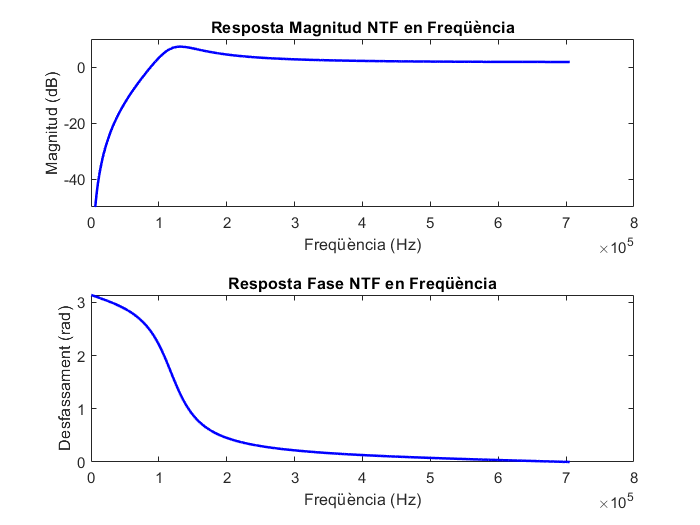
\includegraphics[width=0.5\linewidth]{Images/bodeNTFMOD2.png}
    \caption{Diagrama de Bode de la funció de transferència del Soroll (NTF(z)).}
    \label{figbodeNTF}
\end{figure}

\section{Implementació en codi VHDL}
\par Per a la implementació del modulador s'ha optat per descriure l'entitat en codi VHDL de forma intuïtiva per facilitar la feina de debugging en el procés de validació. 
\par L'estructura del bloc $\Sigma \Delta$ s'ha dissenyat dins de la mateixa sentència \textit{process}, amb només el senyal del rellotge de la FPGA a la llista de sensibilitat. D'aquesta forma, tots els subprocessos que es duen a terme en el modulador s'executen síncrons al rellotge intern de la FPGA. Seguint el diagrama de blocs de la figura \ref{fig_SigmaDelta}, el codi en VHDL s'ha agrupat en subblocs disposats d'esquerra a dreta. Aquesta organització permet tenir una visió més intuïtiva i coherent del que s'està implementant. El codi, tot i que és de creació pròpia, està inspirat en \cite{codiGit}.
\begin{figure}[H]
    \centering
    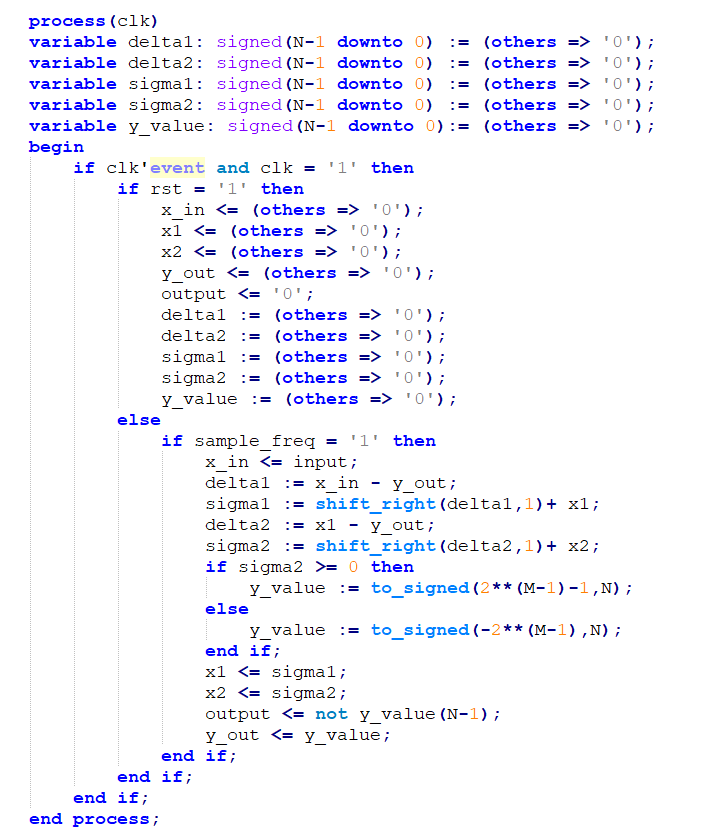
\includegraphics[width=0.5\linewidth]{Images/process_SDM.png}
    \caption{Sentència del \textit{process} on s'executen les operacions del modulador $\Sigma \Delta$.}
    \label{fig_processSDM}
\end{figure}
\begin{figure}[H]
    \centering
    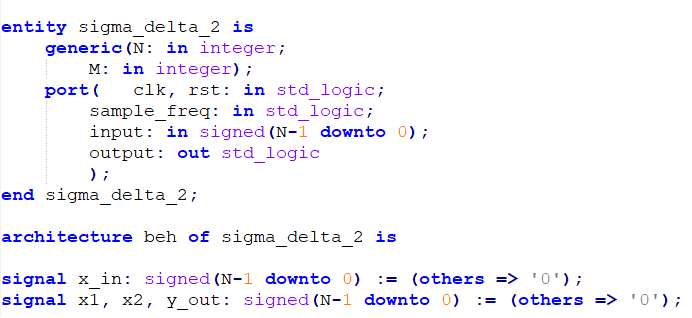
\includegraphics[width=0.5\linewidth]{Images/signals_SDM.png}
    \caption{Declaració de senyals de l'entitat sigma\textunderscore delta\textunderscore2}
    \label{fig_signalsSDM}
\end{figure}
\par Com es pot apreciar a la figura \ref{fig_SigmaDelta}, la sortida dels blocs $\Delta$ s'assigna a una variable \textit{deltaN} i la sortida dels blocs integradors o $\Sigma$, s'assignen a un senyal definida sota la nomenclatura de la variable d'estat visible a la figura \ref{fig_SigmaDelta}. En l'entorn VHDL, les variables dins d'un \textit{process} s'actualitzen en el mateix instant de canviar el seu contingut; no és el cas dels senyals, doncs en VHDL s'actualitzen un cop finalitzat el bloc \textit{process}. Per aquest motiu, els senyals que representen les variables d'estat s'actualitzen un cicle de mostreig més tard, tal i com està definit en l'equació \ref{eq_IntZ}. Per fer una abstracció del que s'està implementant, a la figura \ref{fig_integradordelay} es pot veure l'estructura del bloc integrador.
\begin{figure}[H]
    \centering
    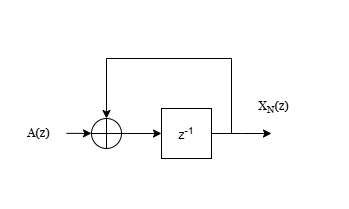
\includegraphics[width=0.5\linewidth]{Images/DelayIntegrator.png}
    \caption{Diagrama de blocs del bloc integrador del modulador $\Sigma \Delta$}
    \label{fig_integradordelay}
\end{figure}
\par El bloc quantificador està implementat de manera que pugui ser configurable el valor dels nivells i no hi hagi desbordament aritmètic en els blocs integradors. Modificant el valor genèric M, és possible definir inicialment el format en coma fixa dels valors a l'entrada. I finalment, la sortida del bloc $\Sigma \Delta$ prové del signe del valor en els llaços de realimentació. És a dir, si el valor al llaç és positiu a la sortida hi haurà un 1 lògic i si el valor al llaç de realimentació és negatiu, a la sortida PDM hi haurà un 0 lògic.

\subsubsection{Validació en testbench}
\par En l'última etapa de la validació del modulador, es dissenya un banc de proves per a l'entitat en VHDL. Per poder comprovar que efectivament el bloc funciona correctament, es genera un senyal sinusoidal de 24 bits amb un fons d'escala de 16 bits i es simulen el senyal de rellotge i el senyal corresponent a la freqüència de mostreig. 
\begin{figure}[H]
    \centering
    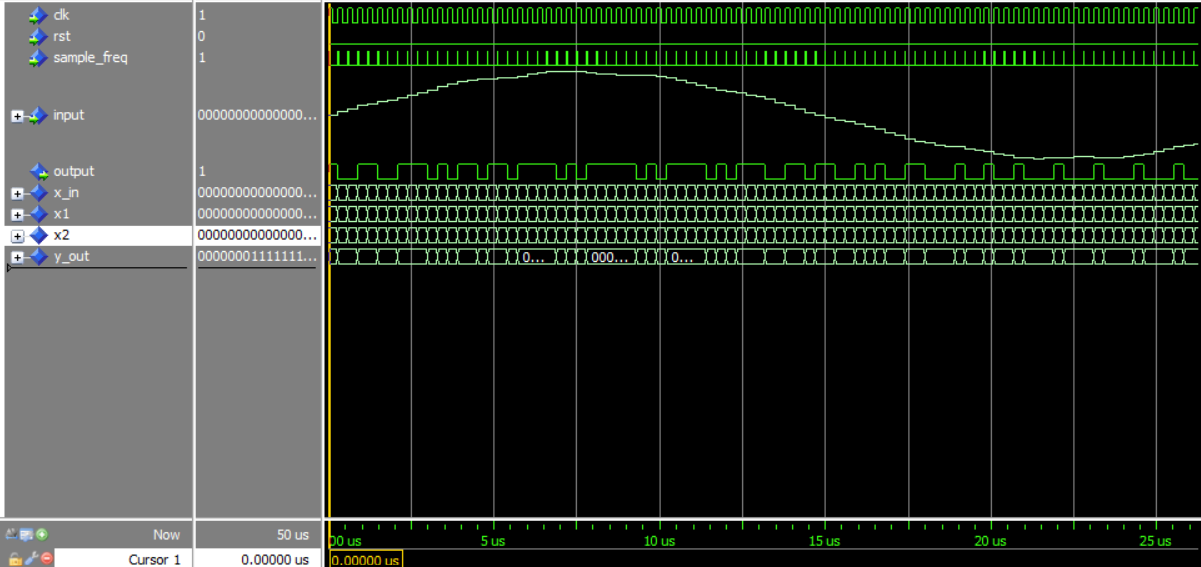
\includegraphics[width=0.7\linewidth]{Images/TestbenchSigmaDelta.png}
    \caption{Diagrama de temps del banc de proves per la validació de l'entitat sigma\textunderscore delta\textunderscore2. En gran es pot apreciar l'ona sinusoidal aplicada a l'entrada i abaix la sortida en format PDM del modulador.}
    \label{figtestbench_SigmaDelta}
\end{figure}
\begin{figure}[H]
    \centering
    \includegraphics[width=0.7\linewidth]{Images/TestbenchSigmaDelta_integrator.png}
    \caption{Diagrama de temps del banc de proves per la validació de l'entitat sigma\textunderscore delta\textunderscore2. De nou, en gran es pot apreciar l'ona sinusoidal aplicada a l'entrada i més avall, les senyals x1 i x2 el valor de les variables d'estat.}
    \label{figtestbench_SigmaDelta2}
\end{figure}

\par Tal com es mostra a les figures \ref{figtestbench_SigmaDelta} i \ref{figtestbench_SigmaDelta2}, el bloc $\Sigma \Delta$ funciona segons el comportament esperat. A la sortida, es pot observar que l'amplada dels polsos varia en funció del senyal sinusoidal.

\section{Implementació a la FPGA}
\par Finalment, s'importa l'entitat dissenyada al programa Vivado per generar el bloc IP que posteriorment s'afegirà al projecte general. A la taula \ref{taularecursosSigma}, es pot visualitzar els recursos emprats de la FPGA per a la implementació del modulador. Destaquen les 228 LUTs i la manca de blocs DSP la qual cosa ens indica que el programa ha sintetitzat el blocs sumadors amb LUTs i registres. Pràctica que no resulta gaire eficient però degut a les dimensions del treball no suposa un impediment per a la implementació en conjunt. 

\begin{table}[H]
    \centering
    \begin{tabular}{ | c | c | c | c | c | c |}
    \hline
    \centering
    \textbf{ID}     &  \textbf{LUTs} & \textbf{Registres}  & \textbf{Slices} & \textbf{Muxes}  & \textbf{DSPs} \\ [2ex] \hline
    \centering
    sigma\textunderscore delta \textunderscore 2    &  228 & 67  & 32 & 0  & 0 \\ \hline
    \end{tabular}
    \caption{Utilització de recursos de la FPGA pel bloc IP dissenyat.}
    \label{taularecursosSigma}
\end{table}
\chapter{Anàlisi de la sostenibilitat i implicacions ètiques del Treball}
\section{Impacte ambiental}
\par Amb l'objectiu d'analitzar el possible impacte ambiental d'aquest treball, s'ha considerat la petjada ecològica directa i indirecta de les implicacions que pot tenir la realització d'aquest treball. 
\par Una de les mesures que s'han pres per reduir l'impacte ambiental, ha sigut reutilitzar components electrònics en desús d'anteriors projectes i utilitzar una placa de desenvolupament que ha sigut utilitzada per altres estudiants per acomplir el treball de fi de grau com el present. A més a més, materials com cables unifilars i una protoboard s'han utilitzat per a l'aplicació de la font d'àudio, els quals són materials que d'acabada la vida útil del projecte, es podràn reutilitzar per altres projectes. Per últim, les eines que s'han utilitzat en el desenvolupament del treball com el multímetre i l'oscil·loscopi, són propietat de la universitat i han sigut utilitzats només el temps que s'ha necessitat per la validació del projecte, permetent que altres estudiants de l'EEBE puguin fer-ne un ús similar.
\par Indirectament, la utilització de certs components com la placa de desenvolupament Nexys4 o la targeta ESP32, inclouen ICs que s'han produit a escala industrial. La producció a gran escala d'aquests components tenen una petjada ecològica associada que és rellevant en la lluita contra el canvi climàtic. Concretament, en \cite{FtprntEco} es fa un estudi detallat de la petjada ecològica per l'extracció de materials semiconductors. Es calcula que pel 2030 les emissions d'aquesta indústria es multiplicarien per 4 en els millors dels casos, superant les produides per altres indústries com la metalúrgica o d'aviació.
\begin{figure}[H]
    \centering
    \includegraphics[width=0.25\linewidth]{Images/graf_ambienta.png}
    \caption{A l'esquerra predicció de les emissions de gasos d'efecte hivernacle de l'Indústria de producció de Semiconductors. A la dreta, les emissions de gasos produides per la indústria química, metal·lúrgica i d'aviació.\cite{FtprntEco}}
    \label{figGrafhivern}
\end{figure}
\par AMD, l'empresa fabricant de la FPGA utilitzada en la implementació d'aquest treball, publica annualment informes dels avenços en la reducció de la emissió de gasos d'efecte hivernacle, amb l'objectiu de contribuir a complir els objectius de l'agenda 2030.\cite{AMDGHG}

\chapter{Pressupost del treball}
\section{Cost retributiu}
\par Per estimar els costos de l'elaboració d'aquest treball cal considerar el temps invertit, les persones involucrades i les respectives retribucions per hores. En l'elaboració d'aquest projecte han participat l'autor del treball i el corresponent tutor en matèria d'assessorament. Conforme \cite{BOEsal}, el SMI per un enginyer tècnic amb graduat universitari és 22224,26 \euro per un any de treball a jornada completa i 14 pagues. S'assigna doncs una retribució horària per l'autor d'aquest treball de 10,68 \euro/h. La realització d'aquest treball implica la dedicació mínima de 24 ECTS, que amb l'equivalència de 25 h/ECTS resulta en 600 hores de dedicació total. 
\begin{table}[H]
    \centering
    \begin{tabular}{ | c | c | c | c |}
    \hline
    \textbf{Cost Retributiu}     &  \textbf{Hores dedicades} & \textbf{Sou}& \textbf{Cost total}\\ [2ex] \hline
    Cost mà d'obra   & 600 h & 10,68 & 6408 \euro \\ \hline
    Cost assessorament  & 9 h & 20 & 180 \euro \\ \hline
    \textsc{TOTAL}    &  -  & - & 6588 \euro \\ \hline
    \end{tabular}
    \caption{Costos en concepte de retribució dels implicats en la realització del present treball.}
    \label{taula_salaris}
\end{table}

\section{Costos dels materials}
\par La implementació física del treball ha requerit un seguit de components i eines amb un cost econòmic. A la taula \ref{taula_material} es detallen els costos dels materials emprats en el desenvolupament del treball. 
\begin{table}
    \centering
    \begin{tabular}{ | c | c | }
    \hline
    \centering
    \textbf{Material}     &  \textbf{Preu de mercat}\\ [2ex] \hline
    \centering
    Targeta ESP32-WROOM    &    11,50 \euro \\ \hline
    \centering
    Adapatador targeta $\mu$SD    &    3,85 \euro \\ \hline
    \centering
    Targeta $\mu$SD    &    3,50 \euro \\ \hline
    \centering
    Mòdul alimentació de 5V i 3,3V    &    4,50 \euro \\ \hline
    \centering
    Placa de desenvolupament NEXYS4    &    412 \euro \\ \hline
    \centering
    Kit protoboards i cables    &    3 \euro \\ \hline
    \centering
    Auricolars amb entrada jack de 3.5 mm    &    7 \euro \\ \hline
    \centering
    \textsc{TOTAL}    &    445,35 \euro \\ \hline
    \end{tabular}
    \caption{Costos en material utilitzat per la implementació del treball.}
    \label{taula_material}
\end{table}

\section{Costos de les eines}
\par A continuació, es procedeix a fer una valoració econòmica de les eines que s'han utilitzat i el temps que s'han emprat. En el còmput global del pressupost del treball, només es considerarà l'amortització. A la taula següent es desglossen les eines emprades:
\begin{table}[H]
    \centering
    \begin{tabular}{ | c | c | c | c | c |}
    \hline
    \centering
    \textbf{Eines}     &  \textbf{Preu de mercat} & \textbf{Vida útil}  & \textbf{Temps d'ús} & \textbf{Amortització}\\ [2ex] \hline
    \centering
    Ordinador Portàtil    &  1000 \euro &  10000 h  &  540 h  &  54 \euro\\ \hline
    \centering
    Multímetre    &    20 \euro &  1000 h  &  10 h  &  0.2 \euro\\ \hline
    \centering
    Oscil·loscopi    &    3270 \euro &  10000 h  &  10 h  &  3,27 \euro\\ \hline
    \centering
    Estació de soldadura   &    420,75 \euro &  5000 h  &  15 min  &  0,02 \euro\\ \hline
    \centering
    \textsc{TOTAL}    &    - &  -  &  -  &  57,49 \euro\\ \hline
    \end{tabular}
    \caption{Costos d'amortització de les eines emprades pel desenvolupament del treball.}
    \label{taula_eines}
\end{table}

\par En el disseny de les etapes de filtratge de l'amplificador de classe D digital s'ha emprat el programa MATLAB\textsuperscript{\tiny\textregistered}, i aquest té un cost de llicència de 119 \euro \ com a preu de partida.\cite{MATLABlic}

\section{Pressupost final}
\par Finalment, es presenta la taula \ref{taula_pressupost} on s'engloben els costos totals del treball implementat.
\begin{table}[H]
    \centering
    \begin{tabular}{ | c | c | }
    \hline
    \centering
    \textbf{Concepte}     &  \textbf{Cost}\\ [2ex] \hline
    \centering
    Cost Retributiu    &    6588 \euro \\ \hline
    \centering
    Costos dels materials    &    445,35 \euro \\ \hline
    \centering
    Costos de les eines \& llicències   &    176,49 \euro \\ \hline
    \centering
    \textsc{TOTAL}    &    7209,84 \euro \\ \hline
    \end{tabular}
    \caption{Pressupost total del treball realitzat.}
    \label{taula_pressupost}
\end{table}
\chapter{Anàlisi final del treball}
\section{Implementació del treball a la FPGA}
\par Finalment, es sintetitzen els blocs documentats en els apartats anteriors i es tracen les connexions necessàries en el diagrama de blocs del projecte de Vivado. El diagrama final es pot veure a l'annex 5. S'adjunten els resultats en l'utilització dels recursos de la FPGA a la taula \ref{taula_recursosFPGA} i l'informe del timing dels processos (\ref{figTiming}) a la FPGA juntament amb el dels consums de potència (\ref{figPWR}).
\begin{figure}[H]
    \centering
    \includegraphics[width=0.6\linewidth]{Images/Timingreport.png}
    \caption{Informe del timing dels processos dins la FPGA.}
    \label{figTiming}
\end{figure}
\begin{figure}[H]
    \centering
    \includegraphics[width=0.4\linewidth]{Images/PWR_FPGA.png}
    \caption{Informe dels consums de potència dels subprocessos en la implementació a la FPGA.}
    \label{figPWR}
\end{figure}
\begin{table}
    \centering
    \begin{tabular}{ | c | c | }
    \hline
    \textbf{Recurs}     &  \textbf{Nombre}\\ [2ex] 
    \hline
    LUTs     &  1170\\
    \hline
    Registres     &  891\\
    \hline
    Slices     &  247\\
    \hline
    Muxes     &  46\\
    \hline
    DSPs     &  4\\
    \hline
    \end{tabular}
    \caption{Utilització de recursos de la FPGA en la implementació final del projecte.}
    \label{taula_recursosFPGA}
\end{table}

\par A la figura \ref{figTiming} es pot observar que el projecte sintetitzat compleix amb els requeriments dels temps de setup dels blocs síncrons, amb un marge positiu de +4,436 ns respecte al temps de setup més crític. Per tant, el sistema no presenta risc de metaestabilitat als blocs interns de la FPGA. En lo referent al consum de la implementació del projecte a la FPGA, el bloc que consumeix més potència és el bloc de gestió del rellotge de la FPGA i només consumeix 100 mW. Per últim, el disseny consumeix menys d'1\% del total dels recursos disponibles del model Artix-7 (\ref{taulaArtix7}).

\section{Resultats experimentals}
\par Per poder validar el projecte implementat, s'ha analitzat la resposta del sistema a una entrada sinusoidal de 1 kHz de freqüència. S'ha utilitzat un arxiu .wav de la sinusoidal samplejada a 44.1 kHz i d'amplada 16 bits \cite{Sin1kHZ} per transmetre-la des de la font d'àudio pel bus I2S i s'ha capturat la sortida PDM i la sortida analògica en un oscil·loscopi.
\begin{figure}[H]
    \centering
    \includegraphics[width=0.7\linewidth]{Images/FFT_in.png}
    \caption{FFT del senyal sinusoidal de 1 kHz a l'entrada.\cite{FFTSin1kHz}}
    \label{figFFTsine}
\end{figure}
\par A la figura \ref{figFFT_tot} es pot observar com la FFT del senyal de sortida en format PDM no és del tot nítida i té una arrissada apreciable en tot l'espectre. A la figura \ref{figPDM_gran}, es pot visualitzar la trama PDM i intuir l'amplada dels respectius polsos.  
\par D'altra banda, la FFT de la sortida analògica es mostra a la figura \ref{figFFT_1kHz} i \ref{fig_FFT2kHz}, on es pot apreciar que el senyal fonamental de 1 kHz té una amplitud similar a la de l'harmònic de 2,5 kHz. Possibles fonts de soroll poden ser la mala connexió de la sonda a l'hora de capturar els senyals i la presència d'elements paràsits en la implementació del test. En conjunt, és plausible que totes les fonts de soroll mencionades influeixin al senyal, reproduint la sortida d'àudio lleugerament distorsionada. 
\par En conclusió, el sistema és capaç de transmetre un senyal d'àudio reconeixible, però amb soroll acoblat a la sortida. En la realització d'aquest treball, no ha donat temps a dissenyar una etapa que ataqui aquesta problèmatica mencionada. 

\begin{figure}
    \centering
    \includegraphics[width=0.5\linewidth]{Images/Setup_test.png}
    \caption{Setup del test pràctic per a la validació final del sistema implementat.}
    \label{figsetup}
\end{figure}

\newpage

\begin{figure}[H]
    \centering
    \includegraphics[width=0.5\linewidth]{Images/FFT_tot.png}
    \caption{FFT de la sortida PDM del sistema.}
    \label{figFFT_tot}
\end{figure}

\begin{figure}[H]
    \centering
    \includegraphics[width=0.5\linewidth]{Images/FFT_1kHz.PDMpng.png}
    \caption{FFT de la sortida PDM del sistema, amb el cursor sobre la freqüència de 1 kHz i 1 MHz.}
    \label{figFFT1kPDM}
\end{figure}

\begin{figure}[H]
    \centering
    \includegraphics[width=0.5\linewidth]{Images/FFT_8kHz.png}
    \caption{FFT de la sortida PDM del sistema, amb el cursor sobre la freqüència de 8,76 kHz i 1 MHz.}
    \label{figFFT8kPDM}
\end{figure}

\begin{figure}[H]
    \centering
    \includegraphics[width=0.5\linewidth]{Images/FFT_5kHz.png}
    \caption{FFT de la sortida PDM del sistema, amb el cursor sobre la freqüència de 5 kHz i 1 MHz.}
    \label{figFFT5kPDM}
\end{figure}

\begin{figure}[H]
    \centering
    \includegraphics[width=0.5\linewidth]{Images/PDM_outgran.png}
    \caption{Trama de la sortida PDM del sistema.}
    \label{figPDM_gran}
\end{figure}

\begin{figure}[H]
    \centering
    \includegraphics[width=0.5\linewidth]{Images/FFT_1kHz.png}
    \caption{FFT de la sortida analògica del sistema, centrat a l'origen de coordenades la freqüència de 1 kHz.}
    \label{figFFT_1kHz}
\end{figure}

\begin{figure}[H]
    \centering
    \includegraphics[width=0.5\linewidth]{Images/FFT_2kHz.png}
    \caption{FFT de la sortida analògica del sistema, centrat a l'origen de coordenades la freqüència de 2,5kHz.}
    \label{fig_FFT2kHz}
\end{figure}

\section{Valoració final dels objectius}
Per concloure la realització d'aquest treball, es recuperen els objectius establerts a l'introducció i es fa una valoració de si s'han complert i de les problemàtiques enfrontades.  

\subsubsection{Objectiu 1}
\begin{quote}
    \textit{Implementar un bloc IP receptor per fer lectures en protocol I2S.}
\end{quote}
\par El primer objectiu s'ha assolit de forma satisfactòria, ja que s'ha pogut implementar un bloc IP d'un receptor del protocol I2S. L'entitat receptora I2S s'ha dissenyat íntegrament en codi VHDL i amb una arquitectura estructural. Com s'ha pogut demostrar al capítol 4, el bloc captura correctament les trames d'àudio que es transmeten pel bus i les guarda al registre de sortida. 
\par No obstant, la validació empírica del bloc ha estat condicionada per la font d'àudio ja que aquesta inicialment no era capaç de transmetre informació pel bus I2S.   

\subsubsection{Objectiu 2}
\begin{quote}
    \textit{Dissenyar i implementar etapes de filtrat per l'àudio a l'entrada i sobremostrejar el senyal.}
\end{quote}
\par El segon objectiu s'ha implementat correctament fent ús dels blocs IP LogiCORE CIC Compiler i FIR Compiler, i configurant-los per complir les especificacions de disseny. 
\par Per contra, l'implementació d'aquesta etapa ha tardat més temps de l'esperat retrassant les altres fases de disseny. Inicialment, es va optar per descriure el procés de filtrat i interpolació en codi VHDL però no es van acabar de resoldre les derives en l'estabilitat del sistema. Finalment es va dessistir en el desenvolupament del codi en VHDL, a favor de completar la realització del treball. 

\subsubsection{Objectiu 3}
\begin{quote}
    \textit{Dissenyar i implementar un modulador $\Sigma \Delta$ que modeli el soroll provocat per la quantificació.}
\end{quote}
\par S'ha complert el tercer objectiu, implementant un modulador $\Sigma \Delta$ de segon ordre. L'entitat s'ha pogut descriure en VHDL al complet, aplicant una modelació del soroll de quantificació efectiva. 
\par En canvi, no s'ha aconseguit implementar un modulador d'ordre superior perquè no s'ha pogut garantir l'estabilitat del sistema. La implementació de moduladors $\Sigma \Delta$ amb més de dos blocs integradors no es pot dur a terme de manera directa, com en el cas d'un modulador de segon ordre, ja que cal considerar la re-ubicació dels nous pols en el sistema per assegurar-ne l'estabilitat. 

\subsubsection{Objectiu 4}
\begin{quote}
    \textit{Dissenyar una etapa de delmat del senyal d'àudio provinent del bloc $\Sigma \Delta$.}
\end{quote}
\par No s'ha pogut assolir el quart objectiu degut a la falta de temps per poder dedicar-li el temps necessari per a la implementació. Momentàneament es va intentar implementar un etapa de filtrat austera amb un bloc IP FIR Compiler, pero malauradament no va funcionar. D'haver fet una gestió més eficient del temps en la realització d'aquest treball, hagués sigut possible dissenyar una etapa de filtrat específica pel senyal en format PDM, a la sortida del bloc $\Sigma \Delta$.
%\printbibliography
\addcontentsline{toc}{chapter}{Bibliografia}
\bibliographystyle{ieeetr}
\bibliography{export.bib}
\appendix
\chapter{Annexos}
\section{Codi ESP32 per transmetre trames d'àudio en protocol I2S}
\begin{lstlisting}[language=C++, basicstyle=\ttfamily\small, breaklines=true, frame=single]
// Codi ESP32 -- Font audio I2S
// Includes

    #include "SD.h"                         
    #include "driver/i2s.h"          
  
//----------------------
//----------------------
// Defines
 
//    SD Card
    #define SD_CS          5    
   
//    I2S

    #define I2S_DOUT      25    
    #define I2S_BCLK      27   
    #define I2S_LRC       26    
    #define I2S_NUM       0    

// Wav Fitxer
    #define NUM_BYTES_TO_READ_FROM_FILE 1024   

//----------------------

//----------------------
// structures and also variables
//  I2S configuration

      static const i2s_config_t i2s_config = 
      {
          .mode = (i2s_mode_t)(I2S_MODE_MASTER | I2S_MODE_TX),
          .sample_rate = 44100,                                
          .bits_per_sample = I2S_BITS_PER_SAMPLE_16BIT,
          .channel_format = I2S_CHANNEL_FMT_RIGHT_LEFT,
          .communication_format = (i2s_comm_format_t)(I2S_COMM_FORMAT_I2S | I2S_COMM_FORMAT_I2S_MSB),
          .intr_alloc_flags = ESP_INTR_FLAG_LEVEL1,             
          .dma_buf_count = 8,                           
          .dma_buf_len = 64,                                    
          .use_apll=0,
          .tx_desc_auto_clear= true, 
          .fixed_mclk=-1    
      };
    
//----------------------
// Pin configuració      
      static const i2s_pin_config_t pin_config = 
      {
          .bck_io_num = I2S_BCLK,              
          .ws_io_num = I2S_LRC,                           
          .data_out_num = I2S_DOUT,                       
          .data_in_num = I2S_PIN_NO_CHANGE                  
      };
      
      struct WavHeader_Struct
      {
          //   RIFF Section    
          char RIFFSectionID[4];    
          uint32_t Size;             
          char RiffFormat[4];         
          
          //   Format Section    
          char FormatSectionID[4];   
          uint32_t FormatSize;       
          uint16_t FormatID;         
          uint16_t NumChannels;       
          uint32_t SampleRate;        
          uint32_t ByteRate;          
          uint16_t BlockAlign;       
          uint16_t BitsPerSample;  
        
          // Data Section
          char DataSectionID[4];      
          uint32_t DataSize;       
      }WavHeader;
//------------------

//  Global Variables/objects    
    
    File WavFile;                                
    static const i2s_port_t i2s_num = I2S_NUM_0;      

//-----------------


void setup() {    
    Serial.begin(115200);                               
    SDCardInit();
    i2s_driver_install(i2s_num, &i2s_config, 0, NULL);
    i2s_set_pin(i2s_num, &pin_config);
    WavFile = SD.open("/audioprova.wav");                   
    if(WavFile==false)
      Serial.println("Could not open 'wavfile.wav'");
    else
    {
      WavFile.read((byte *) &WavHeader,44); 
      DumpWAVHeader(&WavHeader);           
      if(ValidWavData(&WavHeader))    
        i2s_set_sample_rates(i2s_num, 44100);     
    }
}


void loop()
{    
    PlayWav();                                          
}

void PlayWav()
{
  static bool ReadingFile=true;                    
  static byte Samples[NUM_BYTES_TO_READ_FROM_FILE];   
  static uint16_t BytesRead;                          

  if(ReadingFile)                                    
  {
    BytesRead=ReadFile(Samples);                   
    ReadingFile=false;             
  }
  else
    ReadingFile=FillI2SBuffer(Samples,BytesRead);    
}

uint16_t ReadFile(byte* Samples)
{
    static uint32_t BytesReadSoFar=0;                   
    uint16_t BytesToRead;                           
    
    if(BytesReadSoFar+NUM_BYTES_TO_READ_FROM_FILE>WavHeader.DataSize)  
      BytesToRead=WavHeader.DataSize-BytesReadSoFar;          
    else
      BytesToRead=NUM_BYTES_TO_READ_FROM_FILE;             
      
    WavFile.read(Samples,BytesToRead);              
    BytesReadSoFar+=BytesToRead;         
    
    if(BytesReadSoFar>=WavHeader.DataSize)   
    {
      WavFile.seek(44);                    
      BytesReadSoFar=0;                                    
    }
    return BytesToRead;             
}

bool FillI2SBuffer(byte* Samples,uint16_t BytesInBuffer)
{
    
    size_t BytesWritten;                        
    static uint16_t BufferIdx=0;      
    uint8_t* DataPtr;              
    uint16_t BytesToSend;      
    
    DataPtr=Samples+BufferIdx;                               
    BytesToSend=BytesInBuffer-BufferIdx;                     
    i2s_write(i2s_num,DataPtr,BytesToSend,&BytesWritten,1);  
    BufferIdx+=BytesWritten;                          
    
    if(BufferIdx>=BytesInBuffer)                 
    {
      BufferIdx=0; 
      return true;                             
    }
    else
      return false;     
}

void SDCardInit()
{        
    pinMode(SD_CS, OUTPUT); 
    digitalWrite(SD_CS, LOW);
    if(!SD.begin(SD_CS))
    {
        Serial.println("Error talking to SD card!");
        while(true);                  
    }
}

bool ValidWavData(WavHeader_Struct* Wav)
{
  
  if(memcmp(Wav->RIFFSectionID,"RIFF",4)!=0) 
  {    
    Serial.print("Invalid data - Not RIFF format");
    return false;        
  }
  if(memcmp(Wav->RiffFormat,"WAVE",4)!=0)
  {
    Serial.print("Invalid data - Not Wave file");
    return false;           
  }
  if(memcmp(Wav->FormatSectionID,"fmt",3)!=0) 
  {
    Serial.print("Invalid data - No format section found");
    return false;       
  }
  if(memcmp(Wav->DataSectionID,"data",4)!=0) 
  {
    Serial.print("Invalid data - data section not found");
    return false;      
  }
  if(Wav->FormatID!=1) 
  {
    Serial.print("Invalid data - format Id must be 1");
    return false;                          
  }
  if(Wav->FormatSize!=16) 
  {
    Serial.print("Invalid data - format section size must be 16.");
    return false;                          
  }
  if((Wav->NumChannels!=1)&(Wav->NumChannels!=2))
  {
    Serial.print("Invalid data - only mono or stereo permitted.");
    return false;   
  }
  if(Wav->SampleRate>48000) 
  {
    Serial.print("Invalid data - Sample rate cannot be greater than 48000");
    return false;                       
  }
  if((Wav->BitsPerSample!=8)& (Wav->BitsPerSample!=16)) 
  {
    Serial.print("Invalid data - Only 8 or 16 bits per sample permitted.");
    return false;                        
  }
  return true;
}


void DumpWAVHeader(WavHeader_Struct* Wav)
{
  if(memcmp(Wav->RIFFSectionID,"RIFF",4)!=0)
  {
    Serial.print("Not a RIFF format file - ");    
    PrintData(Wav->RIFFSectionID,4);
    return;
  } 
  if(memcmp(Wav->RiffFormat,"WAVE",4)!=0)
  {
    Serial.print("Not a WAVE file - ");  
    PrintData(Wav->RiffFormat,4);  
    return;
  }  
  if(memcmp(Wav->FormatSectionID,"fmt",3)!=0)
  {
    Serial.print("fmt ID not present - ");
    PrintData(Wav->FormatSectionID,3);      
    return;
  } 
  if(memcmp(Wav->DataSectionID,"data",4)!=0)
  {
    Serial.print("data ID not present - "); 
    PrintData(Wav->DataSectionID,4);
    return;
  }  
  Serial.print("Total size :");Serial.println(Wav->Size);
  Serial.print("Format section size :");Serial.println(Wav->FormatSize);
  Serial.print("Wave format :");Serial.println(Wav->FormatID);
  Serial.print("Channels :");Serial.println(Wav->NumChannels);
  Serial.print("Sample Rate :");Serial.println(Wav->SampleRate);
  Serial.print("Byte Rate :");Serial.println(Wav->ByteRate);
  Serial.print("Block Align :");Serial.println(Wav->BlockAlign);
  Serial.print("Bits Per Sample :");Serial.println(Wav->BitsPerSample);
  Serial.print("Data Size :");Serial.println(Wav->DataSize);
}

void PrintData(const char* Data,uint8_t NumBytes)
{
    for(uint8_t i=0;i<NumBytes;i++)
      Serial.print(Data[i]); 
      Serial.println();  
}
\end{lstlisting}

\newpage

\section{\textit{Script} del disseny de l'etapa de filtrat i sobremostreig}
\begin{lstlisting}[language=Matlab, basicstyle=\ttfamily\small, breaklines=true, frame=single]

clc; clear all;

%% Disseny Filtre CIC Interpolador
R = 16;          
M = 1;           
N = 5;          

cicInterp = dsp.CICInterpolator(R,M,N);

freqRange = linspace(0, 3, 2048);

[H, W] = freqz(cicInterp, freqRange);

gain_correction = 1/(R^N);

%% Diagrama de Bode Filtre CIC

figure(1);
tiledlayout;
nexttile;
plot(W/pi, 20*log10(gain_correction * abs(H)), 'b', 'LineWidth', 1.5);
ylim([-150 10]);
title('Filtre CIC Resposta en Freqüència');
xlabel('Freqüència Normalitzada (\times\pi rad/mostra)');
ylabel('Magnitud (dB)');

nexttile;
phaseCIC = phasez(cicInterp,freqRange);
plot(W/pi, phaseCIC, 'b', 'LineWidth', 1.5);
title('Filtre CIC Resposta en Freqüència');
xlabel('Freqüència Normalitzada (\times\pi rad/mostra)');
ylabel('Desfassament (rad)');

%% Disseny Filtre Compensació CIC

fs = 44100;
fPass = 20000;
fStop = 22050;
ast = 80;

CICCompInterp = dsp.CICCompensationInterpolator(cicInterp,...
    InterpolationFactor=2,PassbandFrequency=fPass, ...
    StopbandFrequency=fStop,StopbandAttenuation=ast, ...
    SampleRate=fs)

[H2, W2] = freqz(CICCompInterp, freqRange);

coeff_CompCIC = coeffs(CICCompInterp);
coeff_CompCIC.Numerator(77) = 1;
valors_CICComp = round(coeff_CompCIC.Numerator*power(2,17)-1);

%% Diagrama de Bode Filtre Compensació CIC

figure(2);
tiledlayout;
nexttile;
plot(W2/pi, 20*log10(abs(H2)), 'b', 'LineWidth', 1.5);
ylim([-100 20]);
title('Filtre Compensació Resposta en Freqüència');
xlabel('Freqüència Normalitzada (\times\pi rad/mostra)');
ylabel('Magnitud (dB)');

nexttile;
phaseCICComp = phasez(CICCompInterp,freqRange);
plot(W2/pi, phaseCICComp, 'b', 'LineWidth', 1.5);
title('Filtre Compensació en Freqüència');
xlabel('Freqüència Normalitzada (\times\pi rad/mostra)');
ylabel('Desfassament (rad)');

%%  Etapa de Filtrat Final

FC = dsp.FilterCascade(CICCompInterp, cicInterp);
[H3, W3] = freqz(FC, freqRange);

%% Diagrama de Bode de l'Etapa de filtrat.

figure(3);
tiledlayout;
nexttile;
plot(W3, 20*log10((gain_correction/2) * abs(H3)), 'b', 'LineWidth', 1.5);
ylim([-150 10]);
title('Etapa de Filtrat Resposta en Freqüència');
xlabel('Freqüència (Hz)');
ylabel('Magnitud (dB)');

nexttile;
phaseFC = phasez(FC,freqRange);
plot(W3, phaseFC, 'b', 'LineWidth', 1.5);
title('Etapa de Filtrat Resposta en Freqüència');
xlabel('Freqüència (Hz)');
ylabel('Desfassament (rad)');

%% Càlculs de l'Etapa de filtrat
indH = find((gain_correction/2)*abs(H3) < sqrt(1/2), 1, 'first');
slopeH = (gain_correction/2)*(abs(H3(indH)) - abs(H3(indH - 1))) / (W3(indH) - W3(indH - 1));
w_3dBH = ( sqrt(1/2) - (gain_correction/2)*abs(H3(indH - 1)) + slopeH * W3(indH - 1) )/(slopeH);

f_start = 2*pi()*20/(32*44.1e3); 
f_end = w_3dBH; 
band_idx = (W3 >= f_start & W3 <= f_end); 

mag_dB = 20*log10((gain_correction/2)*abs(H3(band_idx)));


variacion = max(mag_dB) - min(mag_dB);

fprintf('La variación en la banda de paso es %.2f dB\n', variacion);

\end{lstlisting}

\newpage

\section{\textit{Script} del disseny del modulador $\Sigma\Delta$}
\begin{lstlisting}[language=Matlab, basicstyle=\ttfamily\small, breaklines=true, frame=single]

clear all; clc;

syms z w;
Ts = 708.6e-9;
z_freq_tr = cos(w*Ts) + 1i*sin(w*Ts);

%% Gain correction coefficients after delta sub-block in loop filter
a1 = 0.5;
a2 = 0.5;

%% Integrator transfer function
H = 1/(z-1);

%% Noise Transfer Function 2nd order
numNTF = 1;
den = 1 + a2*H + a1*a2*H^2;
NTF = numNTF/den;
NTF1 = collect(NTF);
[numNTF1, den1] = numden(NTF1);
polyNTF = tf(sym2poly(numNTF1), sym2poly(den1), Ts);
[HNTF, WNTF] = freqz(sym2poly(numNTF1), sym2poly(den1),2048,1/Ts);

figure(1);
tiledlayout;
nexttile;
plot(WNTF, 20*log10(abs(HNTF)), 'b', 'LineWidth', 1.5);
ylim([-50 10]);
title('Resposta Magnitud NTF en Freqüència');
xlabel('Freqüència (Hz)');
ylabel('Magnitud (dB)');

nexttile;
phaseNTF = phasez(sym2poly(numNTF1), sym2poly(den1),2048);
plot(WNTF, phaseNTF, 'b', 'LineWidth', 1.5);
title('Resposta Fase NTF en Freqüència');
xlabel('Freqüència (Hz)');
ylabel('Desfassament (rad)');

% bodeNTF = bodeplot(polyNTF);

%% Signal Transfer Function 2nd order
numSTF = a1*a2*H^2;
den2 = 1 + a2*H + a1*a2*H^2;
STF = numSTF/den2;
STF1 = collect(STF);
[numSTF1, den2_1] = numden(STF1);
polySTF = tf(sym2poly(numSTF1), sym2poly(den2_1), Ts);
[HSTF, WSTF] = freqz(sym2poly(numSTF1), sym2poly(den2_1),2048,1/Ts);

figure(2);
tiledlayout;
nexttile;
plot(WSTF, 20*log10(abs(HSTF)), 'b', 'LineWidth', 1.5);
ylim([-50 10]);
title('Resposta Magnitud STF en Freqüència');
xlabel('Freqüència (Hz)');
ylabel('Magnitud (dB)');

nexttile;
phaseSTF = phasez(sym2poly(numSTF1), sym2poly(den2_1),2048);
plot(WSTF, phaseSTF, 'b', 'LineWidth', 1.5);
title('Resposta Fase STF en Freqüència');
xlabel('Freqüència (Hz)');
ylabel('Desfassament (rad)');
% bodeSTF = bodeplot(polySTF);

%% Zero plot for NTF and STF
figure(3);
% pzmap(polyNTF);
% hold on;
% [poles1, zeros1] = pzmap(polySTF);
% [poles2, zeros2] = pzmap(polyNTF);
% for i = 1:length(zeros2)
%     plot(real(zeros2(i)), imag(zeros2(i)), 'ro', 'MarkerSize', 10, 'MarkerFaceColor', 'r');
%     text(real(zeros2(i)), imag(zeros2(i)), sprintf(' Z%d', i), 'VerticalAlignment', 'bottom', 'HorizontalAlignment', 'right', 'Color', 'r');
% end
% 
% % Plot poles with blue crosses and label them
% for j = 1:length(poles2)
%     plot(real(poles2(j)), imag(poles2(j)), 'b', 'MarkerSize', 6, 'LineWidth', 1.5);
%     text(real(poles2(j)), imag(poles2(j)), sprintf(' P%d', j), 'VerticalAlignment', 'top', 'HorizontalAlignment', 'left', 'Color', 'b');
% end
% 
% % Set axis labels and title
% xlabel('Real Part');
% ylabel('Imaginary Part');
% title('Pole-Zero Map with Legends');
% 
% % Add grid and axis limits
% axis equal; % Keep the aspect ratio equal
% xlim([-1.1 1.1]);
% ylim([-1.1 1.1]);
% 
% % Add legend
% legend('Zeros', 'Poles', 'Location', 'best');
% 
% % Hold off to avoid overlaying future plots
% hold off;
pzmap(polySTF, 'ko', polyNTF, 'b');

%% Find poles of both NTF and STF
polesden = solve(den1, z);
stable = abs(double(polesden(1))) < 1

%% Z-domain poles map to frequency domain
pole1_freq = polesden(1) - z_freq_tr; 
pole2_freq = polesden(2) - z_freq_tr;

%% Poles in the frequency domain
wp1 = solve(pole1_freq, w);
wp2 = solve(pole2_freq, w);

%% Corner frequencies 
f01 = abs(double(wp1))/(2*pi());
f02 = abs(double(wp2))/(2*pi());

%% Damping factor
e_rara = -real(double(wp1))/(f01*2*pi());

%% Find cutoff frequency STF
ind = find(abs(HSTF) < sqrt(1/2), 1, 'first');
slope = (abs(HSTF(ind)) - abs(HSTF(ind - 1))) / (WSTF(ind) - WSTF(ind - 1));
w_3dBL = ( sqrt(1/2) - abs(HSTF(ind - 1)) + slope * WSTF(ind - 1) )/(slope);

%% Find cutoff frequency NTF
indH = find(abs(HNTF) > sqrt(1/2), 1, 'first');
slopeH = (abs(HNTF(indH)) - abs(HNTF(indH - 1))) / (WNTF(indH) - WNTF(indH - 1));
w_3dBH = ( sqrt(1/2) - abs(HNTF(indH - 1)) + slopeH * WNTF(indH - 1) )/(slopeH);

\end{lstlisting}

\newpage

\section{Codi VHDL del Modulador $\Sigma\Delta$}
\begin{lstlisting}[language=VHDL, basicstyle=\ttfamily\small, breaklines=true, frame=single]

library IEEE;
use IEEE.std_logic_1164.all;
use IEEE.numeric_std.all;

entity sigma_delta_2 is
	generic(N: in integer;
		M: in integer);
	port(	clk, rst: in std_logic;
		sample_freq: in std_logic;
		input: in signed(N-1 downto 0);
		output: out std_logic
		);
end sigma_delta_2;

architecture beh of sigma_delta_2 is

signal x_in: signed(N-1 downto 0) := (others => '0');
signal x1, x2, y_out: signed(N-1 downto 0) := (others => '0');

begin
	
	process(clk)
	variable delta1: signed(N-1 downto 0) := (others => '0');
	variable delta2: signed(N-1 downto 0) := (others => '0');
	variable sigma1: signed(N-1 downto 0) := (others => '0');
	variable sigma2: signed(N-1 downto 0) := (others => '0');
	variable y_value: signed(N-1 downto 0):= (others => '0');
	begin
		if clk'event and clk = '1' then
			if rst = '1' then
				x_in <= (others => '0');
				x1 <= (others => '0');
				x2 <= (others => '0');
				y_out <= (others => '0');
				output <= '0';
				delta1 := (others => '0');
				delta2 := (others => '0');
				sigma1 := (others => '0');
				sigma2 := (others => '0');
				y_value := (others => '0');
			else
				if sample_freq = '1' then
					x_in <= input;
					delta1 := x_in - y_out;
					sigma1 := shift_right(delta1,1)+ x1;
					delta2 := x1 - y_out;
					sigma2 := shift_right(delta2,1)+ x2;
					if sigma2 >= 0 then
						y_value := to_signed(2**(M-1)-1,N);
					else
						y_value := to_signed(-2**(M-1),N); 
					end if;
					x1 <= sigma1;
					x2 <= sigma2;
					output <= not y_value(N-1);
					y_out <= y_value; 
				end if;
			end if;
		end if;
	end process;
	
end architecture;	
\end{lstlisting}

\section{Diagrama de blocs del Projecte Final de Vivado}
\begin{figure}[H]
    \centering
    \includegraphics[angle=90,origin=c, width=0.5\linewidth]{Images/VivadoDiagramablocs.png}
    \caption{Diagrama de blocs del projecte al Vivado.}
    \label{fig_VivadoDiagramablocs}
\end{figure}



\end{document}